\documentclass[a5paper, 10pt, twoside, bahasa]{report}
\title{Tugas akhir}
\usepackage{graphicx}
\usepackage{comment}
\usepackage{array}
\usepackage{multirow}
\usepackage{rotating}
\usepackage{booktabs}
\usepackage[ruled,lined,commentsnumbered,linesnumbered]{algorithm2e}
\usepackage{algpseudocode}
\usepackage{makeidx}
\makeindex
\usepackage[pdfauthor={Firdaus Nanda Pradanggapasti},bookmarksnumbered,pdfborder={0 0 0}]{hyperref}  
\usepackage[indonesian]{babel}
\usepackage{epsfig}
\usepackage[top=25mm,left=25mm,right=20mm,bottom=25mm]{geometry}
\usepackage{pdflscape}
\usepackage{setspace}  
\usepackage{type1cm}
\usepackage{lettrine}
\usepackage{hyperref}
\usepackage[pageref]{backref}
\usepackage{multirow}
\usepackage{fancyhdr} 		% Untuk pengaturan header dan footer yang lebih kompleks
\usepackage{etoolbox} 		% Untuk melakukan perubahan (patch) command internal LaTeX
\usepackage{url}
\usepackage{longtable}
\usepackage{float}
\floatstyle{boxed}
\newfloat{program}{thp}{lop}
\floatname{program}{Program}
\usepackage[fleqn]{amsmath}
\usepackage{enumitem}
\usepackage{nonfloat}
\usepackage{ulem}
\usepackage[final]{pdfpages}
\usepackage [raggedright]{titlesec}
\usepackage{subcaption}

\usepackage{array}
\usepackage{multicol}
\usepackage{listings}
\usepackage{wrapfig}

% Caption label bold
\usepackage[labelfont=bf]{caption}
\captionsetup{labelfont=bf}

\renewcommand*\descriptionlabel[1]{\hspace\leftmargin$#1$}
\usepackage{enumitem}
\newcommand{\tabitem}{~~\llap{\textbullet}~~}
\definecolor{commentsColor}{rgb}{0.497495, 0.497587, 0.497464}
\definecolor{keywordsColor}{rgb}{0.000000, 0.000000, 0.635294}
\definecolor{stringColor}{rgb}{0.558215, 0.000000, 0.135316}
\setcounter{tocdepth}{4}
\setcounter{secnumdepth}{4}
% Caption label bold
\usepackage[labelfont=bf]{caption}
\captionsetup{labelfont=bf}

% Jarak caption dengan obyek
\captionsetup[figure]{font=small,skip=5pt}
\captionsetup[table]{font=small,skip=5pt}
\captionsetup[lstlisting]{font=small,skip=5pt}

% Caption nama
\renewcommand{\figurename}{Gambar}
\renewcommand{\tablename}{Tabel}
\renewcommand{\lstlistingname}{Kode}

% Buat source code
\usepackage{courier}
\lstset{
	language=Python, 						% Bahasa pengrograman yang digunakan
	basicstyle=\ttfamily \footnotesize,	% Jenis font dalam listing & Ukuran font
	% numbers=left, 						% Posisi angka untuk line-number
	% numberstyle=\footnotesize, 		% Ukuran angka untuk line-numbers
	% stepnumber=1, 						% Jarak setiap line-numbers
	% numbersep=5pt, 					% Ukuran line-numbers
	backgroundcolor=\color{white}, 		% Warna background. Gunakan \usepackage{color} dulu
	commentstyle=\color{commentsColor}\textit,    % comment style
	deletekeywords={...}, 
	keepspaces=true, 
	keywordstyle=\color{keywordsColor}\bfseries,
	otherkeywords={*,...},
	showspaces=false, 					% Show spaces adding particular underscores
	showstringspaces=false, 				% Underline spaces within strings
	showtabs=false, 						% Show tabs within strings adding particular underscores
	frame=single, 						% Tambahkan Frame
	framesep=0.1pt,						% Jarak frame dengan list content keseluruhan
	framexbottommargin=4pt,				% Jarak frame dengan list content bawah
	framextopmargin=4pt,					% Jarak frame dengan list content atas
	framexleftmargin=1pt,				% Jarak frame dengan list content kiri
	framexrightmargin=1pt,				% Jarak frame dengan list content kanan
	tabsize=2, 							% Sets default tabsize to 2 spaces
	captionpos=b,						% Posisi caption
	breaklines=true, 					% Line breaking
	breakatwhitespace=false, 			% Sets if automatic breaks should only happen at whitespace
	stringstyle=\color{stringColor}, % string literal style
	columns=fixed,
	escapeinside={\%*}{*)}				% if you want to add a comment within your code
}

% Untuk cek nomor halaman
\usepackage{changepage}
\usepackage{graphicx}

\usepackage{lipsum}
\hyphenation{meng-gerak-kan mem-per-kenal-kan me-nger-ja-kan sa-ran seg-men be-ru-pa rasp-ber-ry meng-hu-bun-kan ter-sim-pan smart-phone me-nya-ma-kan sin-kro-ni-sa-si ke-ce-pa-tan di-hu-bung-kan sam-bu-ngan me-ru-pa-kan meng-gu-na-kan ber-da-sar-kan di-la-ku-kan di-gu-na-kan di-ban-ding-kan}

% Definisi untuk "halaman sengaja dikosongkan"
\def\kosong{
  \vspace*{\fill}
  \begin{center}\textit{Halaman ini sengaja dikosongkan}\end{center}
  \vfill
}
\patchcmd{\cleardoublepage}{\hbox{}}{\kosong}{}{}

% Tambahkan PDF atau Gambar
\newif\ifpdf
\ifx\pdfoutput\undefined
   \pdffalse
\else
   \pdfoutput=1
   \pdftrue
\fi
\ifpdf
   \usepackage{graphicx}
   \usepackage{epstopdf}
   \DeclareGraphicsRule{.eps}{pdf}{.pdf}{`epstopdf #1}
   \pdfcompresslevel=9
\else
   \usepackage{graphicx}
\fi

% utk itemize yg lebih rapat
\newenvironment{packed_enum}{
\begin{enumerate}[nolistsep]
  \setlength{\itemsep}{0pt}
  \setlength{\parskip}{0pt}
  \setlength{\parsep}{0pt}
}{\end{enumerate}}

% Untuk citation
\newcommand{\tab}[1]{\hspace{.2\textwidth}\rlap{#1}}
\renewcommand*{\backreflastsep}{, }
\renewcommand*{\backreftwosep}{, }
\renewcommand*{\backref}[1]{}
\renewcommand*{\backrefalt}[4]{
  \ifcase #1
    No citations.
  \or
    (Dikutip pada halaman #2).
  \else
    (Dikutip pada halaman #2).
  \fi
}

% Pengaturan penomoran halaman menggunakan package fancyhdr
\fancyhf{} 								% Mengosongkan header dan footer
\renewcommand{\headrulewidth}{0pt} 		% Menghapus garis horizontal pada header
\pagestyle{fancy} 						% Mengubah pagestyle dokumen menjadi fancy
\fancyfoot[CE,CO]{\thepage}				% Footer kanan pada hal. ganjil dan sebaliknya
\patchcmd{\chapter}{plain}{fancy}{}{} 	% Mengubah pagestyle pada chapter menjadi fancy
\patchcmd{\chapter}{empty}{plain}{}{}

% Pengaturan format Chapter dan Section
\titleformat{\chapter}[display]{\bfseries\Large}{BAB \centering\thechapter}{0ex}{\vspace{0ex}\centering}[\vspace{0ex}]
\titleformat{\section}{\bfseries\large}{\MakeUppercase{\thesection}}{1ex}{}
\titlespacing*{\chapter}{0pt}{-4ex}{0pt}
\titlespacing{\section}{0pt}{0pt}{0pt}

\lstdefinestyle{DOS}
{
	backgroundcolor=\color{black},
	basicstyle=\scriptsize\color{white}\ttfamily
}

\begin{document}
\pagenumbering{roman}
\singlespacing
%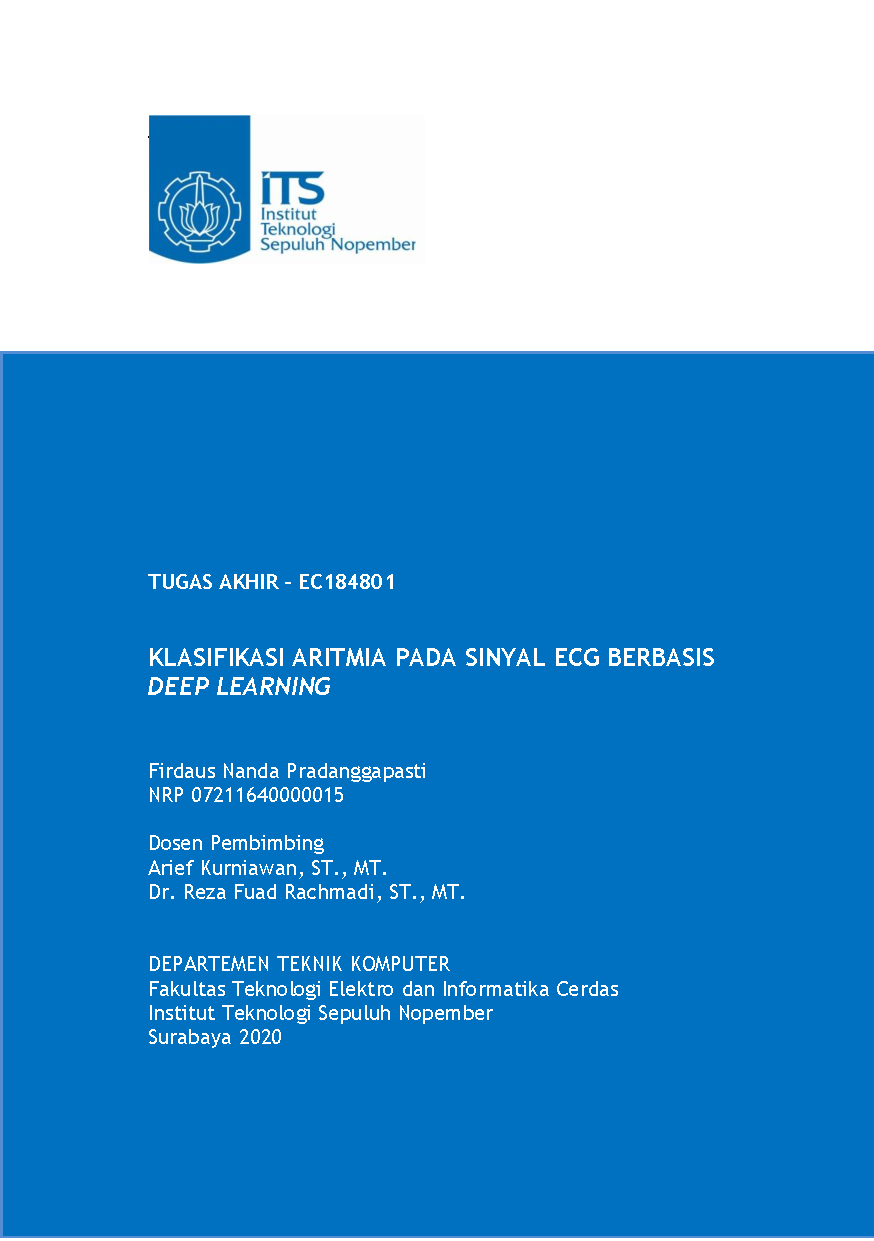
\includepdf[pages=-, offset=0 0]{FileWord/COVER.pdf}
%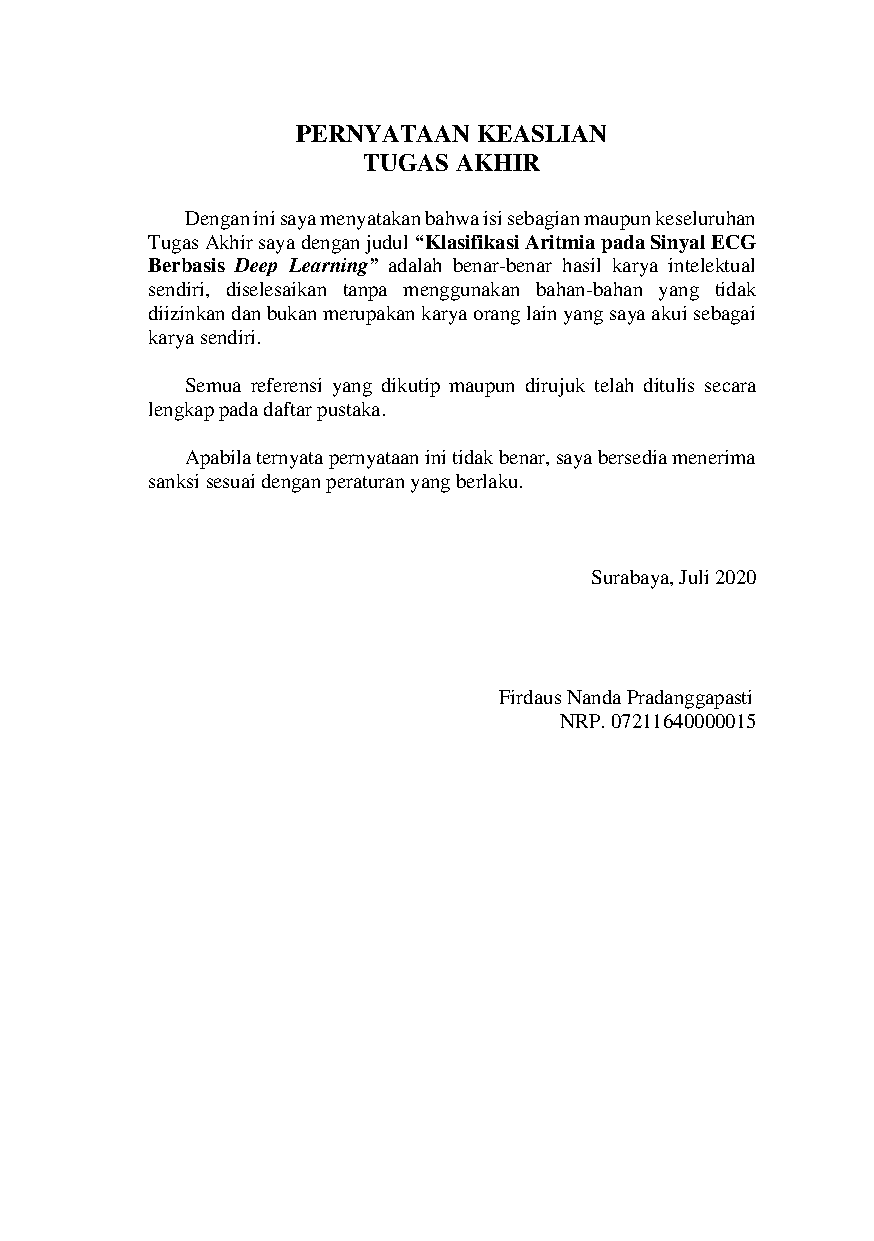
\includepdf[pages=-, offset=0 0]{FileWord/Pernyataan.pdf}
%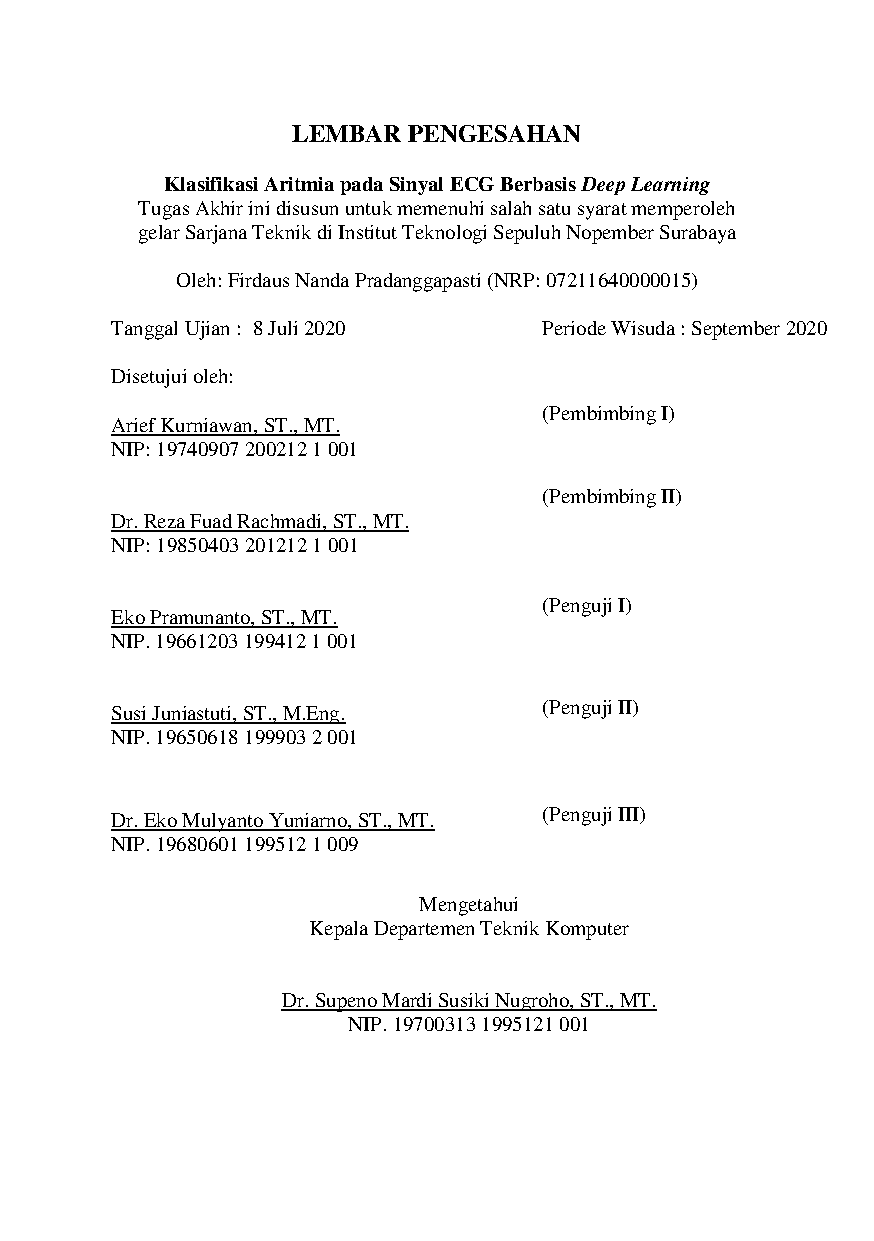
\includepdf[pages=-, offset=0 0]{FileWord/Pengesahan.pdf}

% Sampul luar
\AddToShipoutPictureBG*{
  \AtPageLowerLeft{
    % Ubah nilai berikut jika posisi horizontal background tidak sesuai
    \hspace{-3.5mm}

    % Ubah nilai berikut jika posisi vertikal background tidak sesuai
    \raisebox{0mm}{
      
\includegraphics[width=\paperwidth,height=\paperheight]{sampul/gambar/sampul-luar.png}
    }
  }
}

% Menyembunyikan nomor halaman
\thispagestyle{empty}

% Pengaturan margin untuk menyesuaikan konten sampul
\newgeometry{
  top=95mm,
  left=25mm,
  right=20mm,
  bottom=25mm
}

\begin{flushleft}

  % Pemilihan font sans serif
  \sffamily

  % Pemilihan warna font putih
  \color{white}

  % Pemilihan font bold
  \fontseries{bx}
  \selectfont

  % Ubah penomoran buku berikut dengan yang ditentukan oleh departemen
TUGAS AKHIR - EC184801

\vspace{6ex}

% Ubah kalimat berikut dengan judul tugas akhir
\begin{large}
  APLIKASI TELEKARDIOLOGI UNTUK \textit{MOBILE ANDROID} DILENGKAPI SENSOR ECG
\end{large}

\vspace{4ex}

% Ubah kalimat-kalimat berikut dengan nama dan NRP mahasiswa
Robby Aldriyanto Raffly \\
NRP 0721 17 4000 0011

\vspace{2ex}

% Ubah kalimat-kalimat berikut dengan nama-nama dosen pembimbing
Dosen Pembimbing \\
Arief Kurniawan, ST., MT.\\
Dr. I Ketut Eddy Purnama, ST., MT.

\vspace{6ex}

% Ubah kalimat-kalimat berikut dengan nama departemen dan fakultas
DEPARTEMEN TEKNIK KOMPUTER \\
Fakultas Teknologi ELEKTRO DAN INFORMATIKA CERDAS \\
Institut Teknologi Sepuluh Nopember

% Ubah kalimat berikut dengan tempat dan tahun pembuatan buku
Surabaya 2021


\end{flushleft}

\restoregeometry


% Sampul dalam
\AddToShipoutPictureBG*{
  \AtPageLowerLeft{
    % Ubah nilai berikut jika posisi horizontal background tidak sesuai
    \hspace{-3.5mm}

    % Ubah nilai berikut jika posisi vertikal background tidak sesuai
    \raisebox{0mm}{
      
\includegraphics[width=\paperwidth,height=\paperheight]{sampul/gambar/sampul-dalam.png}
    }
  }
}

% Menyembunyikan nomor halaman
\thispagestyle{empty}

% Pengaturan margin untuk menyesuaikan konten sampul
\newgeometry{
  top=95mm,
  left=25mm,
  right=20mm,
  bottom=25mm
}

\begin{flushleft}

  % Pemilihan font sans serif
  \sffamily

  % Pemilihan font bold
  \fontseries{bx}
  \selectfont

  % Ubah penomoran buku berikut dengan yang ditentukan oleh departemen
TUGAS AKHIR - EC184801

\vspace{6ex}

% Ubah kalimat berikut dengan judul tugas akhir
\begin{large}
  APLIKASI TELEKARDIOLOGI UNTUK \textit{MOBILE ANDROID} DILENGKAPI SENSOR ECG
\end{large}

\vspace{4ex}

% Ubah kalimat-kalimat berikut dengan nama dan NRP mahasiswa
Robby Aldriyanto Raffly \\
NRP 0721 17 4000 0011

\vspace{2ex}

% Ubah kalimat-kalimat berikut dengan nama-nama dosen pembimbing
Dosen Pembimbing \\
Arief Kurniawan, ST., MT.\\
Dr. I Ketut Eddy Purnama, ST., MT.

\vspace{6ex}

% Ubah kalimat-kalimat berikut dengan nama departemen dan fakultas
DEPARTEMEN TEKNIK KOMPUTER \\
Fakultas Teknologi ELEKTRO DAN INFORMATIKA CERDAS \\
Institut Teknologi Sepuluh Nopember

% Ubah kalimat berikut dengan tempat dan tahun pembuatan buku
Surabaya 2021


\end{flushleft}

\restoregeometry

\cleardoublepage

 % Pengaturan ukuran indentasi paragraf
\setlength{\parindent}{2em}

% Pengaturan ukuran spasi paragraf
\setlength{\parskip}{1ex}

% Pernyataan keaslian
\begin{center}
  \large
  \textbf{PERNYATAAN KEASLIAN\\TUGAS AKHIR}
\end{center}

% Menyembunyikan nomor halaman
\thispagestyle{empty}

\vspace{2ex}

% Ubah paragraf-paragraf berikut sesuai dengan yang ingin diisi pada pernyataan keaslian

Dengan ini saya menyatakan bahwa isi sebagian maupun keseluruhan Tugas Akhir sada dengan judul \textbf{"Aplikasi Telekardiologi untuk Mobile Android Dilengkapi Sensor ECG"} adalah benar-benar hasil karya intelektual mandiri, diselesaikan tanpa menggunakan bahan-bahan yang tidak diijinkan da bukan karya pihak lain yang saya akui sebagai karya sendiri.

Semua referensi yang dikutip maupun dirujuk telah ditulis secara lengkap pada daftar pustaka.

Apabila ternyata pernyataan ini tidak benar, saya bersedia menerima sanksi sesuai peraturan yang berlaku.

\vspace{4ex}

\begin{flushright}
  \begin{tabular}[b]{c}
    % Ubah kalimat berikut sesuai dengan tempat, bulan, dan tahun penulisan
    Surabaya, 14 Juni 2021\\
    \\
    \\
    \\
    \\
    % Ubah kalimat-kalimat berikut sesuai dengan nama dan NRP mahasiswa
    Robby Aldriyanto Raffly\\
    0721 17 4000 0011
  \end{tabular}
\end{flushright}

\cleardoublepage

% Lembar pengesahan
%\begin{center}
	\large
  \textbf{LEMBAR PENGESAHAN}
\end{center}

% Menyembunyikan nomor halaman
\thispagestyle{empty}

\begin{center}
  % Ubah kalimat berikut dengan judul tugas akhir
  \textbf{DETEKSI PEJALAN KAKI PADA \textit{ZEBRACROSS} UNTUK PERINGATAN DINI PENGENDARA MOBIL MENGGUNAKAN \textit{MASK R-CNN}}
\end{center}

\begingroup
  % Pemilihan font ukuran small
  \small

  \begin{center}
    % Ubah kalimat berikut dengan pernyataan untuk lembar pengesahan
    Tugas Akhir ini disusun untuk memenuhi salah satu syarat memperoleh gelar Sarjana Teknik di Institut Teknologi Sepuluh Nopember Surabaya
  \end{center}

  \begin{center}
    % Ubah kalimat berikut dengan nama dan NRP mahasiswa
    Oleh: Agung Wicaksonoz (NRP. 0721 17 4000 0002)
  \end{center}

  \begin{center}
    % Ubah kalimat-kalimat berikut dengan tanggal ujian dan periode wisuda
    Tanggal Ujian :  Juli 2021\\
    Periode Wisuda : September 2021
  \end{center}

  \begin{center}
    Disetujui Oleh:
  \end{center}

  \begingroup
    % Menghilangkan padding
    \setlength{\tabcolsep}{0pt}

    \noindent
    \begin{tabularx}{\textwidth}{X c}
      % Ubah kalimat-kalimat berikut dengan nama dan NIP dosen pembimbing pertama
      Prof. Dr. Ir. Mauridhi Hery Purnomo, M.Eng.          & (Pembimbing I) \\
      NIP: 	19580916 198601 1 001       & ................................... \\
      &  \\
      &  \\
      % Ubah kalimat-kalimat berikut dengan nama dan NIP dosen pembimbing kedua
      Dr. Eko Mulyanto Yuniarno, S.T., M.T.     & (Pembimbing II) \\
      NIP: 19680601 199512 1 009        & ................................... \\
      &  \\
      &  \\
      % Ubah kalimat-kalimat berikut dengan nama dan NIP dosen penguji pertama
      %Dr. Galileo Galilei, S.T., M.Sc.  & (Penguji I) \\
      %NIP: 15640215 164201 1 001        & ................................... \\
      &  \\
      &  \\
      % Ubah kalimat-kalimat berikut dengan nama dan NIP dosen penguji kedua
      %Friedrich Nietzsche, S.T., M.Sc.  & (Penguji II) \\
      %NIP: 18441015 190008 1 001        & ................................... \\
      &  \\
      &  \\
      % Ubah kalimat-kalimat berikut dengan nama dan NIP dosen penguji ketiga
      %Alan Turing, ST., MT.             & (Penguji III) \\
      %NIP: 19120623 195406 1 001        & ................................... \\
    \end{tabularx}
  \endgroup

  \vspace{1ex}

  \begin{center}
    % Ubah kalimat berikut dengan jabatan kepala departemen
    Mengetahui, \\
    Kepala Departemen Teknik Komputer FTEIC - ITS \\

    \vspace{7ex}

    % Ubah kalimat-kalimat berikut dengan nama dan NIP kepala departemen
    \underline{Dr. Supeno Mardi Susiki Nugroho, ST., MT.} \\
    NIP. 19700313 199512 1 001
  \end{center}
\endgroup

\cleardoublepage

% Abstrak bahasa indonesia
\setcounter{page}{1}
\addcontentsline{toc}{chapter}{Abstrak}
\begin{center}
\Large\textbf{ABSTRAK}
\end{center}
\vspace{1ex}

\begin{adjustwidth}{-0.2cm}{}
\begin{tabular}{lcp{0.6\linewidth}}
Nama Mahasiswa &:& Robby Aldriyanto Raffly \\
Judul Tugas Akhir &:& Aplikasi Telekardiologi untuk Mobile Android Dilengkapi Sensor ECG \\
Pembimbing &:& 1. Arief Kurniawan, ST., MT. \\
& & 2. Dr. I Ketut Eddy Purnama, ST., MT.  \\
\end{tabular}
\end{adjustwidth}
\vspace{1ex}

\setlength{\parindent}{0cm} Jantung merupakan organ yang sangat penting bagi tubuh. Kematian karena penyakit jantung merupakan salah satu kematian terbanyak di dunia. Penyakit jantung dapat diketahui sejak dini dengan cara memonitoring sinyal detak jantung. Pada Tugas Akhir ini kami mengajukan judul penelitian tentang implementasi sistem telekardiologi. Implementasi sistem telekardiologi yang kami ajukan adalah membuat aplikasi android yang dapat digunakan untuk mengambil data sinyal ECG dari arduino melalui modul bluetooth HC-05. Sinyal ECG tersebut didapatkan arduino dengan menggunakan sensor AD8232. Aplikasi juga memiliki fitur untuk mengirimkan sinyal ECG kepada dokter spesialis jantung sehingga dokter dapat mendiagnosa sinyal ECG pasien tanpa harus mengecek pasien dengan bertemu secara langsung. Aplikasi juga memiliki fitur chat dengan dokter agar pasien dapat berkonsultasi jarak jauh. Hasil yang diharapkan dari penelitian ini adalah aplikasi dapat mengambil data melalui komunikasi bluetooth, mengirimkan data sinyal ECG kepada dokter, dan chatting.

\vspace{2ex}

Kata Kunci : Telekardiologi, ECG, Pengolahan Sinyal, Aplikasi Mobile
\newpage
\cleardoublepage

% Abstrak bahasa ingris
\addcontentsline{toc}{chapter}{Abstract}
\begin{center}
\Large\textbf{ABSTRACT}
\end{center}
\vspace{1ex}

\begin{adjustwidth}{-0.2cm}{}
\begin{tabular}{lcp{0.6\linewidth}}
\textit{Name} &:& Robby Aldriyanto Raffly\\
\textit{Title} &:& \textit{Telecardiology App for Android Mobile Equipped with ECG Sensor} \\
\textit{Advisors} &:& 1. Arief Kurniawan, ST., MT. \\
& & 2. Dr. I Ketut Eddy Purnama, ST., MT. \\
\end{tabular}
\end{adjustwidth}
\vspace{1ex}

	\setlength{\parindent}{0cm}
	\textit{The heart is a very important organ for the body. Death from heart disease is one of the most common deaths in the world. Heart disease can be detected early by monitoring the heartbeat signal. In this final project, we propose a research title on the implementation of telecardiology systems. The implementation of the telecardiology system that we propose is to create an android application that can be used to retrieve ECG signal data from Arduino via the HC-05 bluetooth module. The ECG signal is obtained by Arduino using the AD8232 sensor. The application also has a feature to send an ECG signal to a cardiologist so that doctors can diagnose a patient's ECG signal without having to check the patient in person. The application also has a chat feature with doctors so that patients can consult remotely. The expected result of this research is that the application can retrieve data via bluetooth communication, send ECG signal data to doctors, and chat.} 
	\vspace{2ex}
	
	\textit{Keywords : Telecardiology, ECG, Signal Processing, Mobile Apps}
	\newpage

\cleardoublepage

% Kata pengantar
\addcontentsline{toc}{chapter}{KATA PENGANTAR} % kata pengantar
\begin{center}
\Large\textbf{KATA PENGANTAR}
\end{center}
\vspace{1ex}

\setlength{\parindent}{0.9cm} Puji dan syukur kehadirat Tuhan Yang Maha Esa atas segala karunia-Nya, penulis  dapat menyelesaikan penelitian ini dengan judul \textbf{Aplikasi Telekardiologi untuk Mobile Android Dilengkapi Sensor ECG}.
\vspace{1ex}

Penelitian ini disusun dalam rangka pemenuhan bidang riset di Departemen Teknik Komputer ITS, Bidang  Studi Telematika, serta digunakan sebagai persyaratan menyelesaikan pendidikan  S1. Oleh karena itu, penulis mengucapkan terima kasih kepada:
\vspace{1ex}

\begin{enumerate}[nolistsep]
  \item Keluarga, Ibu, Ayah, dan Saudara tercinta yang telah memberikan dorongan spiritual dan material dalam penyelesaian buku penelitian ini.
  \item Bapak Dr. Supeno Mardi Susiki Nugroho, ST., MT. selaku Kepala Departemen Teknik Komputer, Fakultas Teknik Elektro dan Informatika Cerdas, Institut Teknologi Sepuluh Nopember.
  \item Bapak Arief Kurniawan, ST., MT. selaku dosen pembimbing I dan Bapak Dr. I Ketut Eddy Purnama, ST., MT. selaku dosen pembimbing II yang selalu memberikan arahan selama mengerjakan penelitian tugas akhir ini.  
  \item Bapak-ibu dosen pengajar Departemen Teknik Komputer, atas pengajaran, bimbingan, serta perhatian yang diberikan kepada penulis selama ini.
  \item Seluruh teman-teman dari angkatan e57, Teknik Komputer, Laboratorium B401, dan B201 Teknik Komputer ITS.
\end{enumerate}
\vspace{1ex}

Kesempurnaan hanya milik Allah SWT, untuk itu penulis memohon segenap kritik dan saran yang  membangun. Semoga penelitian ini dapat memberikan manfaat bagi kita semua. Amin.
\begin{flushright}
\begin{tabular}[b]{c}
  Surabaya, Maret 2021
  \\
  \\
  \\
  \\
  Robby Aldriyanto Raffly
\end{tabular}
\end{flushright}
\cleardoublepage

% Daftar isi
\renewcommand*\contentsname{DAFTAR ISI}
\addcontentsline{toc}{chapter}{\contentsname}
\titlespacing*{\chapter}{0pt}{-4ex}{2ex}
\tableofcontents	
\cleardoublepage

% Daftar gambar
\renewcommand*\listfigurename{DAFTAR GAMBAR}
\addcontentsline{toc}{chapter}{\listfigurename}
\titlespacing*{\chapter}{0pt}{-4ex}{2ex}
\listoffigures
\cleardoublepage

% Daftar tabel
\renewcommand*\listtablename{DAFTAR TABEL}
\addcontentsline{toc}{chapter}{\listtablename}
\titlespacing*{\chapter}{0pt}{-4ex}{2ex}
\listoftables
\cleardoublepage

% Nomenklatur
\addcontentsline{toc}{chapter}{NOMENKLATUR}
\begin{center}
	\Large\textbf{NUMENKLATUR}
\end{center}
\vspace{1ex}

\begin{tabular}{c m{30em}}
	$TP$ & : \textit{True Positive}\\
	$TN$ & : \textit{True Negative}\\
	$FP$ & : \textit{False Positive}\\
	$FN$ & : \textit{False Negative}
\end{tabular}
\vspace{1ex}
\cleardoublepage

% BAB isi buku
\titleformat{\chapter}[display]{\bfseries\Large}{BAB \centering\thechapter}{0ex}{\vspace{0ex}\centering}[\vspace{0ex}]
\titleformat{\section}{\bfseries\large}{\MakeUppercase{\thesection}}{1ex}{}
\titleformat{\subsection}{\bfseries\large}{\MakeUppercase{\thesubsection}}{1ex}{}
\titleformat{\subsubsection}{\bfseries\large}{\MakeUppercase{\thesubsubsection}}{1ex}{}
\titlespacing*{\chapter}{0pt}{-4ex}{0pt}
\titlespacing{\section}{0pt}{0pt}{0pt}
\titlespacing{\subsection}{0pt}{0pt}{0pt}
\titlespacing{\subsubsection}{0pt}{0pt}{0pt}

% Indent paragraph
\setlength{\parindent}{0.8cm}

% Penambahan halaman kosong otomatis
\chapter{PENDAHULUAN}
\pagenumbering{arabic}
\vspace{1ex}

\section*{}
Penelitian ini dilatarbelakangi oleh berbagai kondisi yang menjadi acuan. Selain itu juga terdapat beberapa permasalahan yang akan dijawab sebagai luaran dari penelitian.
\vspace{1ex}

\section{Latar belakang}
\vspace{1ex}

Telekardiologi berasal dari kata tele yang berarti jarak jauh dan kardiologi yang merupakan suatu cabang kedokteran yang berhubungan dengan studi dan perawatan kelainan-kelainan di sistem kardiovaskular, yaitu jantung, pembuluh darah, dan pembuluh nadi\cite{cit:1}. Penyakit jantung merupakan penyakit yang menjadi penyebab utama kematian secara global dalam 15 tahun terakhir. Dari 56,9 juta kematian di seluruh dunia pada tahun 2016, lebih dari setengah (54\%) disebabkan oleh 10 penyebab teratas. Penyakit jantung iskemik dan stroke adalah pembunuh terbesar di dunia, yang apabila digabungkan jumlahnya menyebabkan  15,2 juta kematian pada tahun 2016 \cite{cit:2}. Penyakit kardiovaskular juga menjadi penyebab kematian nomor satu di Indonesia. Data dari Institute for Health Metrics and Evaluation, lembaga statistik kesehatan asal Amerika Serikat menyebutkan jumlah kematian akibat penyakit ini mencapai 36,3 persen dari total kematian di Indonesia pada 2016. Selanjutnya, kanker dan diabetes menjadi penyakit yang juga menimbulkan banyak kematian. Indonesia sendiri mendapat peringkat ke-3 di ASEAN setelah Laos dan Filiphine dalam hal jumlah kematian yang disebabkan penyakit kardiovaskular pada tahun 2016 \cite{cit:3}. Salah satu cara untuk mengurangi resiko kematian yang disebabkan penyakit kardiovaskular adalah melakukan pemeriksaan jantung sejak dini. Pemeriksaan kesehatan jantung dapat menggunakan Electrocardiogram (ECG).\

\hspace{2mm} Electrocardiogram adalah tes yang menggunakan alat elektrokardiograf yang dapat menunjukkan seberapa cepat jantung seseorang berdetak, dimana denyut jantung tersebut berupa impulse listrik yang diukur oleh sensor. ECG digunakan untuk menampilkan aktivitas pada jantung, sehingga tenaga medis dapat mendiagnosis apakah detak jantung pada pasien tersebut normal atau tidak. Pemeriksaan rekaman ECG biasanya hanya dapat dilakukan
dilakukan di rumah sakit dengan fasilitas lengkap. Hal tersebut membuat pasien jantung menjadi malas untuk memeriksakan kesehatan jantungnya ke Rumah Sakit. Terlebih lagi disaat kondisi pandemi COVID 19. Rumah Sakit merupakan salah satu tempat yang beresiko menyebabkan penyebaran virus COVID 19. Maka dari itu dibutuhkan sebuah sistem telekardiologi menggunakan aplikasi android agar pasien dan dokter dapat melakukan pemeriksaan secara online tanpa harus pergi ke Rumah Sakit. 

\vspace{1ex} 

\section{Perumusan Masalah}
\vspace{1ex}

Pemeriksaan rekaman ECG masih dilakukan secara offline di Rumah Sakit. Kondisi pandemi COVID 19 menyebabkan Rumah Sakit menjadi tempat yang beresiko penyebaran virus. Oleh karena itu, dibutuhkan sistem telekardiologi dengan menggunakan aplikasi android yang dapat digunakan pasien untuk mengambil sinyal ECG dan mengirim data sinyal ECG kepada dokter spesialis sehingga pasien dapat berkonsultasi dirumah pribadi.

\vspace{1ex}

\section{Tujuan}
\vspace{1ex}

Adapun tujuan dari penelitian Tugas Akhir ini adalah membuat membuat aplikasi android untuk mengambil data ECG melalui bluetooth dan mengirimkan data ECG tersebut kepada dokter spesialis jantung.
\vspace{1ex}

\section{Batasan masalah}
\vspace{1ex}
Batasan masalah yang timbul dari permasalahan Tugas Akhir ini adalah:
\vspace{1ex}
\begin{enumerate}[nolistsep]
	\item Tujuan utama penelitian ini adalah membuat aplikasi yang dapat merekam data ECG, mengirim data ECG, menampilkan grafik ECG, dan \textit{chatting}. 
	\vspace{1ex}
	
	\item Kegiatan uji adalah menampilkan gambar sinyal pada aplikasi android dan melakukan chatting antara pasien dengan dokter.
	\vspace{1ex}
	
	\item Data ECG diambil dari jantung penulis dan alat simulator.
		 
\end{enumerate}
\vspace{1ex}

\section{Sistematika Penulisan}
\vspace{1ex}
Laporan penelitian Tugas akhir ini tersusun dalam sistematika dan terstruktur sehingga mudah dipahami dan dipelajari oleh pembaca maupun seseorang yang ingin melanjutkan penelitian ini. Alur sistematika penulisan laporan penelitian ini yaitu:
\vspace{1ex}

\begin{enumerate}[nolistsep]
	\item BAB I Pendahuluan

	Bab ini berisi uraian tentang latar belakang permasalahan, penegasan dan alasan pemilihan judul, sistematika laporan, tujuan dan metodologi penelitian.
	\vspace{1ex}

	\item BAB II Dasar Teori

	Pada bab ini berisi tentang uraian secara sistematis teori-teori yang berhubungan dengan permasalahan yang dibahas pada penelitian ini. Teori-teori ini digunakan sebagai dasar dalam penelitian, yaitu informasi singkat mengenai sinyal ECG, \textit{Mobile Programming}, aritmia, dan elektrokardiogram.
	\vspace{1ex}

	\item BAB III Perancangan Sistem dan Impementasi

	Bab ini berisi tentang penjelasan-penjelasan terkait eksperimen yang akan dilakukan dan langkah-langkah data diolah hingga menghasilkan visualisasi. Guna mendukung eksperimen pada penelitian ini, digunakanlah blok diagram atau \textit{work flow} agar sistem yang akan dibuat dapat terlihat dan mudah dibaca untuk implementasi pada pelaksaan tugas akhir.
	\vspace{1ex}

	\item BAB IV Pengujian dan Analisa

	Bab ini menjelaskan tentang pengujian eksperimen yang dilakukan terhadap data dan analisanya. Beberapa teknik visualisasi akan ditunjukan hasilnya pada bab ini dan dilakukan analisa terhadap hasil visualisasi dan informasi yang didapat dari hasil mengamati visualisasi yang tersaji.
	\vspace{1ex}

	\item BAB V Penutup

	Bab ini merupakan penutup yang berisi kesimpulan yang diambil dari penelitian dan pengujian yang telah dilakukan. Saran dan kritik yang membangun untuk pengembangkan lebih lanjut juga dituliskan pada bab ini.
\end{enumerate}
\vspace{1ex}
\cleardoublepage
\chapter{TINJAUAN PUSTAKA}
\vspace{1ex}

\section*{}
Demi mendukung penelitian ini, dibutuhkan beberapa teori penunjang sebagai bahan acuan dan referensi. Dengan demikian penelitian ini menjadi lebih terarah. 
\vspace{1ex}

\section{Dasar Teori}
\vspace{1ex}

\subsection{Kardiologi}
\vspace{1ex}
Kardiologi merupakan cabang ilmu kedokteran yang mana dikhususkan mempelajari tentang gangguan jantung dan pembuluh darah. Dokter spesialis yang telah mempelajari kardiologi biasa disebut kardiolog. Akan tetapi kita harus membedakan antara kardiolog dengan ahli bedah jantung, \textit{Cardiothoracic} dan \textit{cardiovascular}, serta ahli bedah yang dapat melakukan bedah jantung menggunakan cara sternotomi. Apabila dibandingkan dengan kardiolog, ahli bedah jantung dapat melakukan operasi dengan cara membuka rongga dada kemudian melaksanakan bedah jantung, sedangkan kardiolog tidak melakukan operasi bedah, namun melakukan tes dan prosedur lain seperti angioplasti.
Kardiologi kemudian dikembangkan lagi menjadi beberapa bagian, yaitu: 
\begin{enumerate}
	\vspace{-2mm}
	\item Ekokardiografi, merupakan metode pemeriksaan jantung yang menggunakan ultrasound (gelombang suara berfrekuensi tinggi) yang dapat menangkap gambaran struktur organ jantung. Ekokardiografi biasanya dibantu dengan teknologi Doppler yang dapat mengukur kecepatan dan arah aliran darah,
	\vspace{-2mm}
	\item Elektroifisiologi Kardiak, merupakan bidang yang mempelajari sifat listrik dan kondisi penyakit jantung, serta pengobatan kelainan irama jantung (aritmia),
	\vspace{-2mm}
	\item Kardiologi Intervensional, merupakan metode perawatan jantung non-bedah yang menggunakan tabung fleksibel kecil atau kateter untuk memperbaiki struktur jantung yang rusak atau tersumbat. Beberapa prosedur yang dapat dilakukan pada jantung dengan cara kateterisasi antara lain: Angioplasti, intervensi koroner perkutan, dan valvuloplasti, 
	\vspace{-2mm}
	\item Kardiologi Nuklir, merupakan metode pemeriksaan jantung menggunakan alat nuklir yang dapat memvisualkan isotop jantung dengan menggunakan radioaktif.
	\vspace{-2mm}
\end{enumerate}
 \vspace{1ex}
 
 Dokter spesialis (kardiolog) bertugas menangani bermacam-macam gangguan terkait jantung dan sistem pembuluh darahnya. Spesifik mengenai kardiologi, jantung memiliki beberapa bagian anatomi (antara lain; atrium, ventrikel, katup) dan beberapa fitur fisiologis (antara lain; sistol, suara) yang mana telah didokumentasikan selama ratusan tahun lalu. Gangguan pada jantung dapat juga berarti mengalami sakit jantung dan sakit kardiovaskuler. Penyakit jantung dan pembuluh darah dapat mengakibatkan jumlah kematian yang cukup signifikan. Penyakit kardiovaskuler telah menyebabkan sekitar 30\%. Persentase tersebut merupakan angka yang cukup tinggi,  Karena jantung memiliki peran yang amat penting bagi tubuh yaitu memompa darah ke seluruh tubuh. Hal tersebut berarti keadaan jantung terhubung dan juga mempengaruhi seluruh keadaan tubuh. Apabila jantung memiliki masalah atau gangguan, maka tubuh juga akan terpengaruh.
 \vspace{1ex}
 
 Kardiologi telah berkembang sejak ratusan tahun lalu. Beberapa catatan kuno telah menjelaskan sedikit bahasan mengenai jantung. Pada 1241, Ibnu Sina dikomentari  oleh Ibn al-Naiis yang mana menyebut tentang sirkulasi darah saat berkomentar. Kemudian tahun 1628, dokter William Harvey dari Inggris adalah orang yang dapat menggambarkan secara tepat bagaimana sistem sirkulasi dan kandungan darah yang dipompa ke seluruh tubuh oleh jantung. Pada 1706, Profesor anatomi Raymond de Vieussens dari Prancis dapat menggambarkan struktur ruang serta pembuluh yang ada pada jantung. Beliau merupakan dokter pertama yang dapat menggambarkan bilik kiri jantung secara akurat. Kemudian pada 1733, Biarawan Stephen Hales, beliau merupakan orang pertama yang dapat mengukur tekanan darah. Perkembangan selanjutnya pada 1816, dokter René-Tnéophile-Hyacinthe Laennec berasal Prancis merupakan orang yang berhasil membuat stetoskop untuk mendiagnosis sejumlah infeksi pada rongga dada. Pada awal abad ke-19 berkembang sedikit moderen, dokter Willem Einthoven dari Belanda pada 1903 mengembangkan elektrokardiograf (ECG atau EKG) sehingga beliau berhasil meraih penghargaan Nobel Kedokteran pada 1924. Dokter Iames Bryan Herrick dari Amerika, pada 1912, beliau merupakan orang yang dapat menggambarkan gejala penyakit jantung \cite{cit:12}.
\vspace{1ex}





\subsection{ECG atau EKG}
\vspace{1ex}

Elektrokardiogram atau EKG merupakan tes yang bertujuan untuk mengukur serta merekam sinyal listrik pada jantung. Sedangkan alat yang digunakan untuk mendeteksi sinyal litrik yang dihasilkan jantung dinamakan elektrokardiograf. Elektrokardiograf dapat membaca sinyal listrik dan kemudian menggambarkan menjadi grafik yang dapat ditampilkan pada layar monitor. Metode elektrokardiogram merupakan metode yang  aman dan tidak menyakitkan karena dilakukan tanpa memberi aliran listrik secara langsung dan tidak memberi sayatan (noninvasif), serta metode ini juga tidak memakan waktu yang lama \cite{cit:13}. 

\subsection{Jenis ECG}
\vspace{1ex}

Berikut merupakan beberapa jenis tes ECG yang biasa dilakukan:
\begin{enumerate}
	\vspace{-2mm}
	\item \textit{Cardiopulmonary exercise test} (CPET)
	\vspace{1ex}
		
	CPET merupakan tes yang biasa dilakukan untuk mendeteksi penyakit jantung atau paru-paru. Saat tes CPET sedang berlangsung, pasien melakukan tes sambil berolahraga ringan dengan sepeda tegak dan bernafas melalui corong. Setiap napas pasien juga akan diukur untuk dinilai seberapa baik kinerja pada tubuh.
	Kekuatan dan kapasitas paru-paru juga diukur dan direkam terlebih dahulu sebelum berolah raga, selama berolah raga, dan sesudah berolahraga.
	Secara total, lama waktu yang diperlukan untuk tes CPET adalah sekitar 40 menit. Untuk waktu berolahraga yang dihabiskan pasien kurang lebih adalah 10 menit. Tes CPET membutuhkan upaya maksimal yang dilakukan pasien agar dapat memperoleh data yang paling bagus atau benar \cite{cit:14}.
	\vspace{-2mm}
	\item \textit{Exercise electrocardiogram (stress test)}
	\vspace{1ex}
	
	Sama seperti tes CPET, tes stress juga dilakukan pasien sambil berolahraga dengan mengayuh sepeda statis atau dengan berjalan diatas treadmill. 
	Tes Stress memiliki tujuan untuk memantau kondisi selama keadaan stres. Tes stress biasanya dilakukan setelah pasien mengalami serangan jantung, operasi jantung, dan juga saat terdeteksi mengalami penyakit arteri koroner \cite{cit:14}.
	\vspace{-2mm}
	\item \textit{Monitor Holter}
	\vspace{1ex}
	
	Holter merupakan jenis perangkat yang dapat dipakai untuk mendapat impuls listrik dari jantung yang bisa digunakan untuk memantau keadaan jantung selama 24 jam atau lebih. Elektroda ditempatkan sesuai tempat tertentu pada dada, lengan, dan kaki.
	Elektroda tersebut terhubung dengan mesin elektrokardiograf melalui kabel timah, sehingga aktivitas jantung dapat dideteksi, divisualisasikan dan kemudian dicetak untuk diinformasikan kepada dokter \cite{cit:14}.
	\vspace{-2mm}
	\item \textit{Resting}12-lead EKG
	\vspace{1ex}
	
	Resting 12-lead EKG merupakan tes yang ideal mengetahui sinyal listrik dari keadaan jantung pasien. Tes ini dilakukan saat keadaan rest atau tidak beraktivitas yang mana pasien menjalani tes ini sambil diam berbaring, setelah itu perangkat 12-lead EKG akan mengukur aktivitas kelistrikan jantung melalui 12 elektroda ysng dipasang pada dada, lengan, dan kaki pasien secara bersamaan.
	Tes ini merupakan jenis yang dapat dipakai secara rutin untuk memantau kondisi jantung sebelum gejala berkembang \cite{cit:14}.
	\vspace{-2mm}
	\item \textit{Signal-averaged electrocardiogram }(SAECG)  
	\vspace{1ex}
	
	Tes SAECG merupakan jenis dengan teknik elektrokardiografi khusus, di mana beberapa sinyal listrik dari jantung dirata-ratakan untuk menghilangkan interferensi dan mengungkapkan variasi kecil pada kompleks QRS, biasanya disebut "potensial akhir". Ini mungkin merupakan kecenderungan terhadap \textit{ventricular tachyarrhythmias} yang berpotensi berbahaya. Tes SAECG dilakukan selama kurang lebih 20 menit untuk mendeteksi adanya aritmia dalam durasi pendek \cite{cit:14}.
\end{enumerate}

\subsection{Sinyal ECG}
\begin{figure}[H]
	\begin{center}\centering
		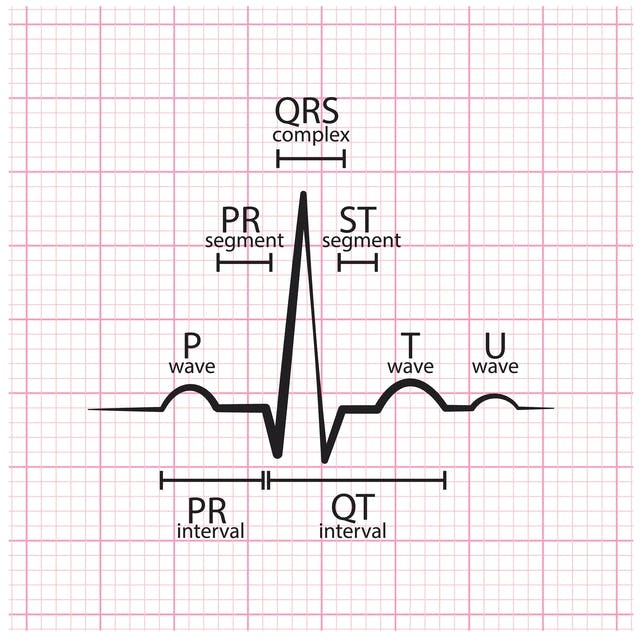
\includegraphics[scale=0.3]{img/Sinyal ecg}
		\caption{Gelombang ECG.}
		\label{fig:2.0}
	\end{center}
\end{figure}

Sinyal atau gelombang ECG merupakan gambaran atau visualisasi data dari aktivitas kelistrikan pada jantung yang telah diukur menggunakan sensor ECG. Gelombang ECG normal terdiri dari 3 bagian dasar. Yang pertama adalah gelombang P (sebelum lonjakan) yang mana menggambarkan aktivitas pada atrium yang memeras darah ke bawah menuju ventrikel. Kedua adalah QRS kompleks yang tampak seperti lonjakan menggambarkan mewakili dua ventrikel yang memeras darah ke tubuh dan paru-paru. Dan yang ketiga adalah gelombang T pada posisi terakhir mencerminkan pemulihan ventrikel saat menjadi rileks untuk menerima darah lagi\cite{cit:10}.
\vspace{1ex}


\subsection{AD8232}
\vspace{1ex}
\begin{figure}[H]
	\begin{center}\centering
		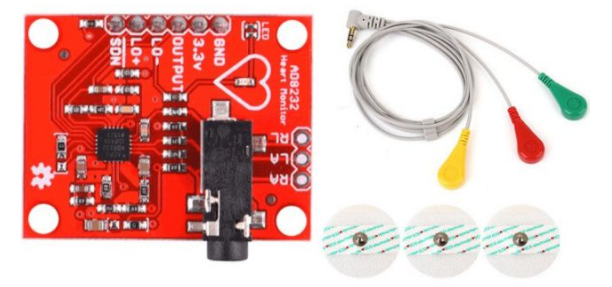
\includegraphics[scale=0.7]{img/AD8232}
		\caption{Sensor AD8232.}
		\label{fig:2.1}
	\end{center}
\end{figure}

AD8232 adalah sensor yang dapat mendeteksi sinyal terintegrasi yang bisa dipakai untuk tes pengukuran detak jantung dan aplikasi pengukuran biopotensial lainnya. AD8232 menggunakan IC pada yang terpasang pada boardnya yaitu modul SEN-12650, modul tersebut memiliki jack 3.5 female yang berfungsi untuk menancapkan kabel elektroda. AD8232 dirancang agar dapat mengekstrak, memperkuat, dan memfilter sinyal biopotensial kecil di hadapan kondisi bising, seperti suara yang dibuat oleh gerakan tubuh. Modul AD8232 memiliki sembilan pin, yaitu SDN, LO +, LO-, OUTPUT, 3.3V, GND, dan juga disediakan pin RA (Lengan Kanan), LA (Lengan Kiri), dan RL (Kaki Kanan) yang dapat dihubungkan dengan tambahan sensor AD8232 yang lain untuk membuat custom jumlah leadnya. Selain itu, modul AD8232 memiliki lampu indikator LED yang akan berkedip mengikuti irama detak jantung\cite{cit:5}.
 
\vspace{1ex}

\subsection{AD8232 \textit{Placement}}
\vspace{1ex}

Dengan modul AD8232, elektroda dihubungkan melalui jack audio. Output buffer dan filter tersedia melalui output analog yang dapat dibaca oleh input analog pada mikrokontroler. Berikut ini merupakan 2 macam penempatan electrode yang ditunjukkan pada Gambar \ref{fig:2.1.0}.
\begin{figure}[H]
	\begin{center}\centering
		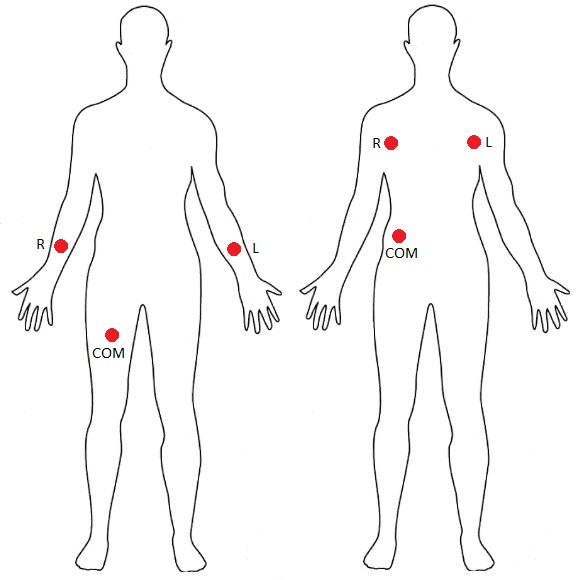
\includegraphics[scale=0.5]{img/AD8232-Electrode-Placement-1}
		\caption{Penempatan AD8232 1 (kiri), Penempatan AD8232 2 (kanan)}
		\label{fig:2.1.0}
	\end{center}
\end{figure}
Berdasarkan gambar tersebut, terdapat 2 macam penempatan electrode. Perbedaan penempatan tersebut tidak mempengaruhi data yang dihasilkan sensor sehingga pengguna bebas memilih salah satu penempatan electrode berdasarkan gambar tersebut.
Elektroda mendeteksi perubahan listrik yang terjadi saat jantung melewati proses detak jantung. Elektroda mendeteksi sinyal listrik kecil yang berada dalam kisaran beberapa ratus mikrovolt ke monitor EKG yang memproses sinyal. Pemrosesan melibatkan amplifikasi dan penyaringan dan kemudian data disediakan dalam format yang dapat digunakan untuk memperbarui tampilan dari beberapa jenis \cite{cit:22}.
\vspace{1ex}

\subsection{Modul Bluetooth HC-05}
\vspace{1ex}

Modul Bluetooth HC-05 merupakan konverter Bluetooth ke serial yang dapat digunakan untuk menghubungkan antara mikrokontroler (seperti Arduino) dengan perangkat berkemampuan Bluetooth lainnya. Pinout dan deskripsi HC-05 adalah seperti berikut:
\begin{enumerate}
	\vspace{-2mm}
	\item \textbf{KEY/En}, Pin ini digunakan untuk membawa modul Bluetooth dalam mode perintah AT. Secara default, pin ini beroperasi dalam mode data. Pin Kunci/EN harus tinggi untuk mengoperasikan Bluetooth dalam mode perintah. Di HC-05, kecepatan baud default dalam mode perintah adalah 38400bps dan 9600 dalam mode data,
	\vspace{-2mm}
	\item \textbf{VCC}, Digunakan untuk memberi daya pada modul Bluetooth. Berikan 5V / 3,3 V ke Pin ini,
	\vspace{-2mm}
	\item \textbf{GND}, Pin ground dari modul,
	\vspace{-2mm}
	\item \textbf{TXD}, Hubungkan pin ini dengan pin RXD Mikrokontroler. Pin ini mentransmisikan data Serial (sinyal nirkabel yang diterima oleh modul Bluetooth diubah oleh modul dan ditransmisikan secara serial pada pin ini),
	\vspace{-2mm}
	\item \textbf{RXD}, Hubungkan pin ini ke pin TXD Mikrokontroler. Modul Bluetooth HC-05 menerima data dari pin ini dan kemudian mentransmisikannya secara nirkabel,
	\vspace{-2mm}
	\item \textbf{State}, Ini digunakan untuk memeriksa apakah modul terhubung atau tidak. Ini bertindak sebagai indikator status.
\end{enumerate}

Modul Bluetooth HC-05 dapat digunakan dalam dua mode operasi: Mode Perintah dan Mode Data. Modus Perintah,
dalam Mode Perintah kita dapat berkomunikasi dengan modul Bluetooth melalui AT Commands untuk mengonfigurasi berbagai pengaturan dan parameter Modul. Ini termasuk informasi firmware, mengubah Baud Rate, mengubah nama modul, dll. Kita juga dapat menggunakannya untuk mengatur HC-05 sebagai master atau slave. Untuk memilih salah satu mode, kita perlu mengaktifkan Mode Perintah dan mengirimkan Perintah AT yang benar. Baud rate defaultnya adalah 38400bps dalam mode perintah .

Modus Data,
dalam mode ini modul digunakan untuk berkomunikasi dengan perangkat Bluetooth lain, yaitu transfer data terjadi dalam mode ini. Pertukaran data antar perangkat. Baud rate defaultnya adalah 9600bps dalam mode data \cite{cit:20}.

\vspace{1ex}


\subsection{Arduino Nano}
\vspace{1ex}


  \begin{table}[h]
 	\begin{tabular}{|l|l|}
 		
 		\hline
 		\multicolumn{1}{|c|}{{\color[HTML]{000000} \textbf{Spesification}}} & \multicolumn{1}{c|}{\textbf{Values}} \\ \hline
 		Microcontroller & Atmel ATmega168 for Arduino \\& Nano 2.x,  \\ 
 		& Atmer ATmega328 for Arduino \\& Nano 3.x \\ \hline
 		Operating voltage & 5 Volt \\ \hline
 		Input voltage & Optimal: 7-12 Volt \\& Min: 6 Volt\\& Max: 20 Volt \\ \hline
 		Digital I/O pins & 14 pins (D0-D13) \\ \hline
 		Analog pins & 8 pins (A0-A7) \\ \hline
 		Maximum electric current & 40 mA \\ \hline
 		Clock speed & 16 Mhz \\ \hline
 		SRAM &  1 kbyte (ATmega168) \\& and 2 kbyte (ATmega328) \\ \hline
 		EEPROM & 512 byte (Atmega168) \\& and 1 kbyte (Atmega328) \\ \hline
 		Flash memory & 32 Mbyte for Arduino Nano 3.x
 		
 		\\& 16 Mbyte for Arduino Nano 2.xz \\ \hline
 		Board size & 4,5 mm x 18 mm \\ \hline
 		Weight & 5 grams \\ \hline	
 		
 	\end{tabular}
 	\vspace{1ex}
 	\caption{Spesifikasi Arduino Nano \cite{cit:19}}
 	\label{tabel:2.0}
 \end{table}
 Perangkat Arduino yang digunakan pada penelitian ini yaitu Arduino Nano. Hal ini karena pada penelitian ini hanya memfokuskan untuk mengirimkan data sinyal dari arduino kepada dokter melalui aplikasi. Berdasarkan hal tersebut maka pada penelitian ini tidak membutuhkan banyak port untuk arduino. Perlu diketahui bahwa pada penelitian ini hanya membutuhkan 1 port analog untuk dihubungkan dengan pin output dari sensor AD8232. Arduino memiliki port ADC yang mana dapat mengkonversi sinyal analog menjadi digital. Pada Arduino Nano terdapat 8 port analog (A0-A7).  Spesifikasi dari Arduino Nano dapat dilihat pada Tabel \ref{tabel:2.0}.
 \clearpage
 

\vspace{1ex}






\section{Penelitian Terkait}
\vspace{1ex}

\subsection{\textit{IoT based Real Time ECG Monitoring System using Cypress WICED}}
\vspace{1ex}
Pada tahun 2017, Uttam U. Deshpande dan Milan A. Kulkarni mengerjakan penelitian, penelitian tersebut merancang dan menerapkan sistem pemantauan ECG berdasarkan \textit{Cypress Wireless Internet Connectivity for Embedded Devices} (WICED) dan membandingkannya dengan  Wi-Fi, Bluetooth, Zigbee dan BLE untuk membuktikan kecepatannya mengirim data yang lebih tinggi dan memiliki cakupan area yang lebih luas.\cite{cit:4}
\vspace{1ex}

\subsection{\textit{An IoT-cloud Based Wearable ECG Monitoring System for Smart Healthcare}}
\vspace{1ex}

Pada tahun 2016, Zhe Yang, Qihao Zhou, Lei Lei, Kan Zheng, dan Wei Xiang melakukan penelitian, yang mana merancang dan menerapkan sistem pemantauan EKG berdasarkan teknik IoT cloud. Penetian ini juga menggunakan Wi-Fi, Bluetooth, Zigbee dan BLE untuk mengirim data ke cloud. Cloud IoT bertanggung jawab untuk memvisualisasikan data EKG kepada pengguna dan menyimpan data untuk analisis lebih lanjut, yang diimplementasikan atas dasar tiga server, yaitu server HTTP, Server MQTT, dan server penyimpanan.\cite{cit:7}
\vspace{1ex}


\cleardoublepage
\chapter{DESAIN DAN IMPLEMENTASI}
\vspace{1ex}

\section*{}
	Penelitian ini dilaksanakan sesuai dengan desain sistem berikut dengan implementasinya. Desain sistem merupakan konsep dari pembuatan dan perancangan infrastruktur kemudian diwujudkan dalam bentuk blok-blok alur yang harus dikerjakan. Pada bagian implementasi merupakan pelaksanaan teknis untuk setiap blok pada desain sistem.
\vspace{1ex}

\section{Desain Sistem}
\vspace{1ex}
Penelitian ini merupakan penerapan dari bidang studi \textit{Mobile
Programming, Internet of Things, Signal processing}, dan Basis data. Penitian ini memiliki tujuan untuk
mengakuisisi data sinyal jantung menggunakan sensor AD8232 dan menyimpan data sinyal tersebut kedalam databse untuk dapat ditampilkan pada aplikasi smartphone pasien dan dokter sehingga dokter dapat memantau kondisi pasien serta memberikan diagnosa, dokter dan pasien juga dapat berkonsultasi melalui fitur chat yang ada pada aplikasi android. Berikut merupakan desain sistem dari penelitian ini.

\vspace{1ex}

\begin{figure}[H] \centering
	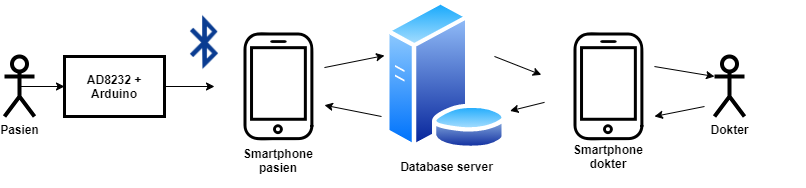
\includegraphics[width=0.9\textwidth]{img/arsitektur.png}
	
	(a)
	
	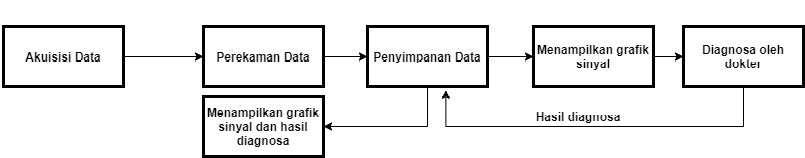
\includegraphics[width=0.9\textwidth]{img/blockdiagram.png}
	
	(b)
	
	\caption{Arsitektur (a) dan Blok Diagram (b) Alur Kerja Sistem}
	\label{fig:3.1}
\end{figure}
\vspace{1ex}

Gambar \ref{fig:3.1} merupakan arsitektur dan
blok diagram alur kerja sistem. Aplikasi android menjadi dapat
mengambil data sinyal jantung pasien yang telah dideteksi
oleh sensor AD8232 melalui modul bluetooth HC-05. Aplikasi
dapat mengirimkan data sinyal jantung pasien kepada dokter
spesialis serta terdapat fitur chatting agar pasien dapat berkonsultasi dengan dokter.
Penelitian ini memiliki bagian tahapan-tahapan yaitu:
\begin{enumerate}
	\vspace{-2mm}
	\item Akuisisi data menggunakan sensor AD8232,
	\vspace{-2mm}
	\item Pengiriman data ECG menuju aplikasi melalui bluetooth HC-05,
	\vspace{-2mm}
	\item Menyimpan data ECG kedalam database,
	\vspace{-2mm}
	\item Menampilkan grafik ECG pada aplikasi android,
	\vspace{-2mm}
	\item Menambahkan fitur chat pada aplikasi android,
	\vspace{-2mm}
	\item Pengujian sistem secara keseluruhan.
\end{enumerate}
\vspace{1ex}

\section{Desain Perangkat}
\vspace{1ex}

Pada penelitian ini menggunakan 3 buah komponen yaitu Arduino Nano, modul bluetooth HC-05, dan sensor AD8232. Rangkaian ketiga komponen tersebut ditunjukkan oleh gambar berikut.
\begin{figure}[H] \centering
	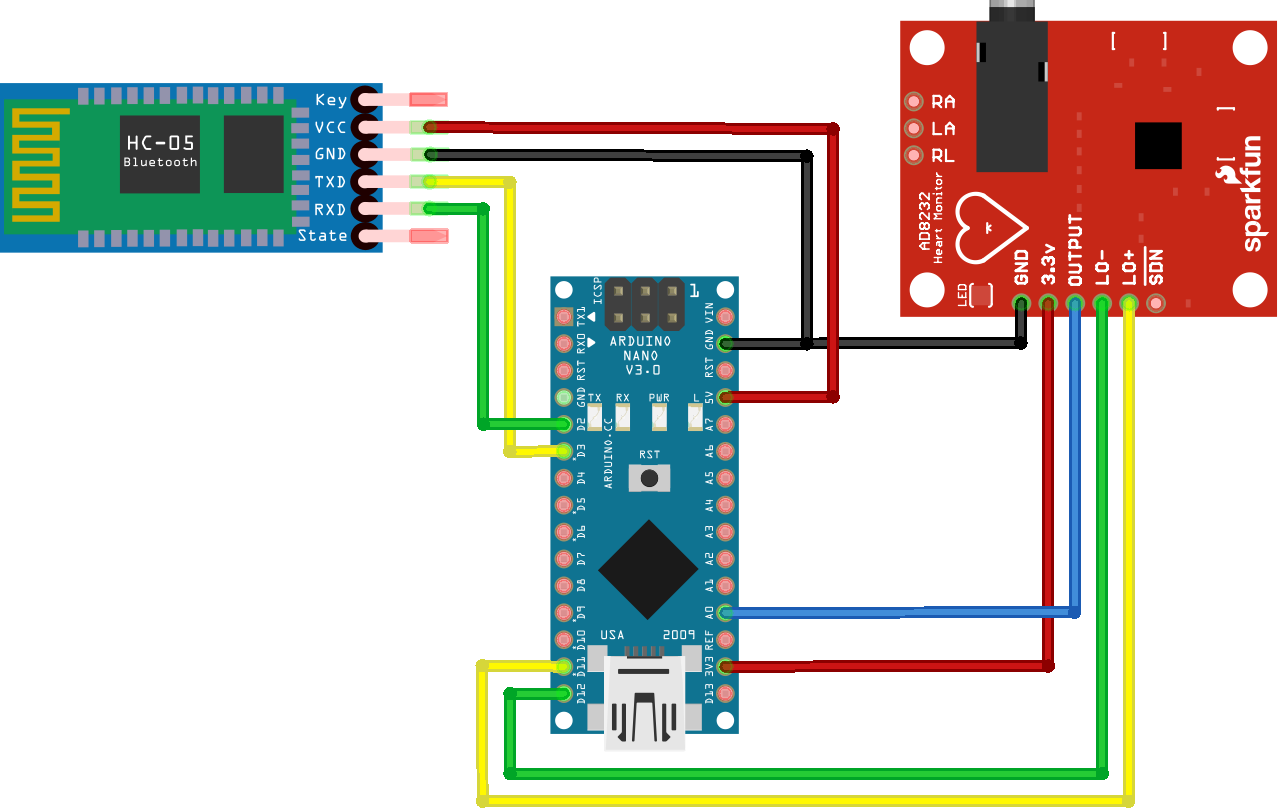
\includegraphics[width=0.9\textwidth]{img/desainperangkat.png}
	\caption{Desain Perangkat ECG}
	\label{fig:3.2.0}
\end{figure}
\vspace{1ex}

Berdasarkan gambar \ref{fig:3.2.0} dapat dilihat sensor AD8232 ada pada posisi paling kanan yang memiliki board berwarna merah. Port AD82332 yang dihubungkan ke Arduino Nano adalah ground, VCC 3.3 Volt, output, LO+, dan LO-. Kemudian pada modul bluetooth HC-05 terdapat 4 port yang dihubungkan pada Arduino Nano yaitu RXD, TXD, GND, dan VCC sebesar antata 3.6 Volt sampai dengan 6 Volt. 
\section{Desain UI Aplikasi}
\vspace{1ex}
Aplikasi android memiliki 2 desain yaitu untuk dokter dan
pasien. Desain UI aplikasi untuk pasien memiliki fitur tambahan. Pada aplikasi pasien memiliki fitur untuk merekam sinyal
ECG sedangkan pada aplikasi dokter tidak disediakan fitur tersebut. Desain aplikasi dokter
ditunjukkan pada Gambar \ref{fig:3.2}.  

\begin{figure}[H] \centering
	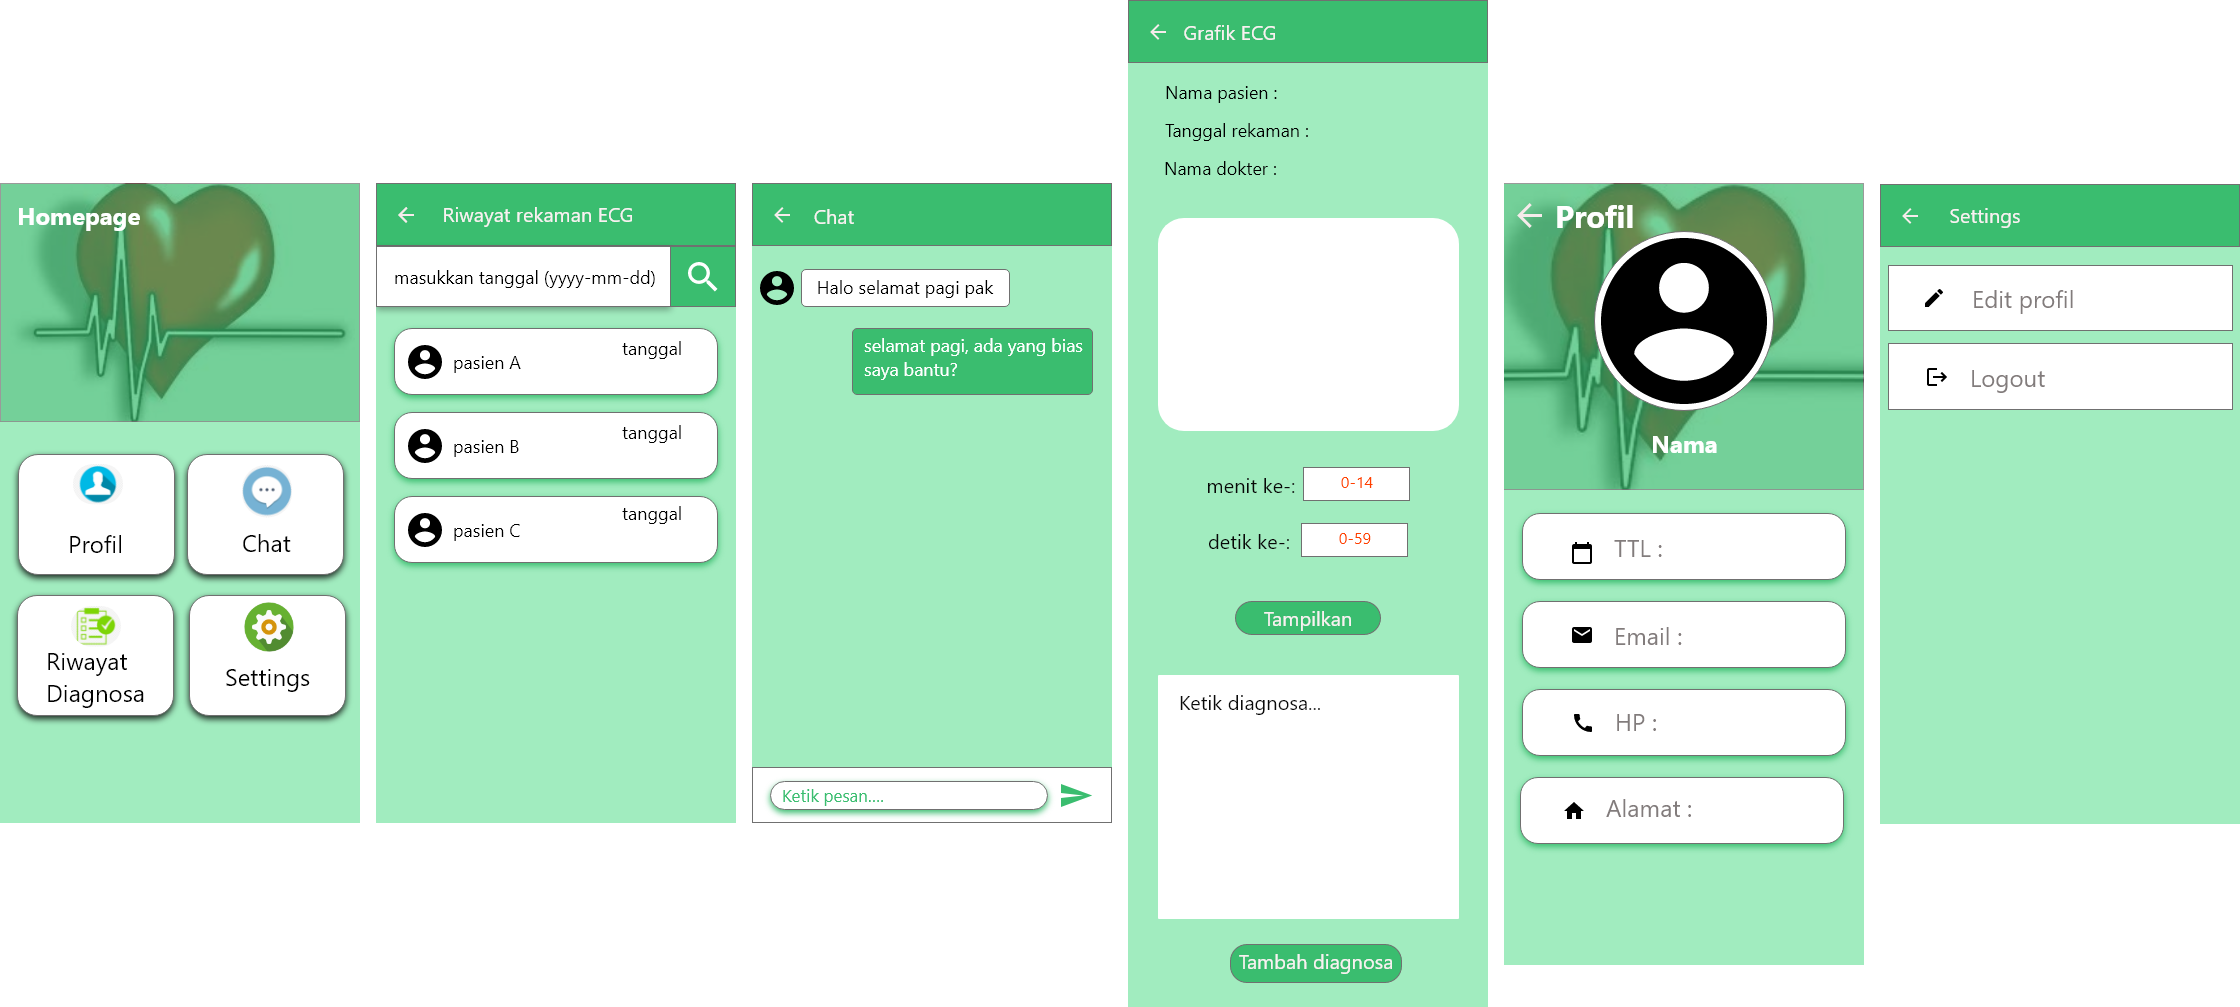
\includegraphics[width=1\textwidth]{img/dokterUI.png}
	\caption{Desain UI pada aplikasi dokter.}
	\label{fig:3.2}
\end{figure}
\vspace{1ex}

Dapat diketahui dari desai UI dokter tersebut terdapat 6 screen, yaitu:
\begin{enumerate}
	\vspace{0mm}
	\item Homepage screen, yang mana merupakan halaman utaman pada aplikasi. Pada Homepage screen dokter tersedia empat buah menu yaitu Profil untuk berpindah ke halaman profil, Chat untuk berpindah ke halaman chat, Riwayat Diagnosa untuk berpindah halaman menuju riwayat diagnosa, dan Settings untuk berpindah ke halaman settings,
	\vspace{0mm}
	\item Riwayat rekaman ECG screen, yang mana merupakan halaman penelusuran yang dapat mencari riwayat ECG pasien pada waktu yang telah diinputkan. Pada screen ini terdapat field untuk menginputkan waktu rekaman dan tombol search untuk mulai mencari. Riwayat rekaman akan ditampilkan dalam bentuk list,
	\vspace{0mm}
	\item Chat screen, yang mana merupakan halaman untuk melakukan komunikasi dengan pasien melalui sebuah pesan,
	\vspace{0mm}
	\item Grafik ECG screen, yang mana merupakan halaman yang dapat menampilkan grafik data ECG hasil rekaman pasien. Pada halaman ini terdapat fitur untuk menampilkan grafik ECG pada waktu tertentu sesuai menit dan detik yang telah diinputkan. Pada halaman ini juga terdapat form isian yang merupakan tempat dokter menambahkan diagnosa untuk pasien,
	\vspace{0mm}
	\item Profil screen, yang mana merupakan halaman yang berisi tentang informasi pengguna. Informasi tersebut antara lain adalah foto, nama lengkap, tanggal lahir, email, nomor telepon, dan alamat,
	\vspace{0mm}
	\item Settings screen, yang mana merupakan halaman yang berisi menu untuk mengubah informasi pada halaman profil dan juga terdapat menu \textit{logout} untuk keluar dari aplikasi.
\end{enumerate}

\clearpage
Berikutnya adalah desain UI untuk pasien ditunjukkan pada Gambar \ref{fig:3.3}.
\begin{figure}[H] \centering
	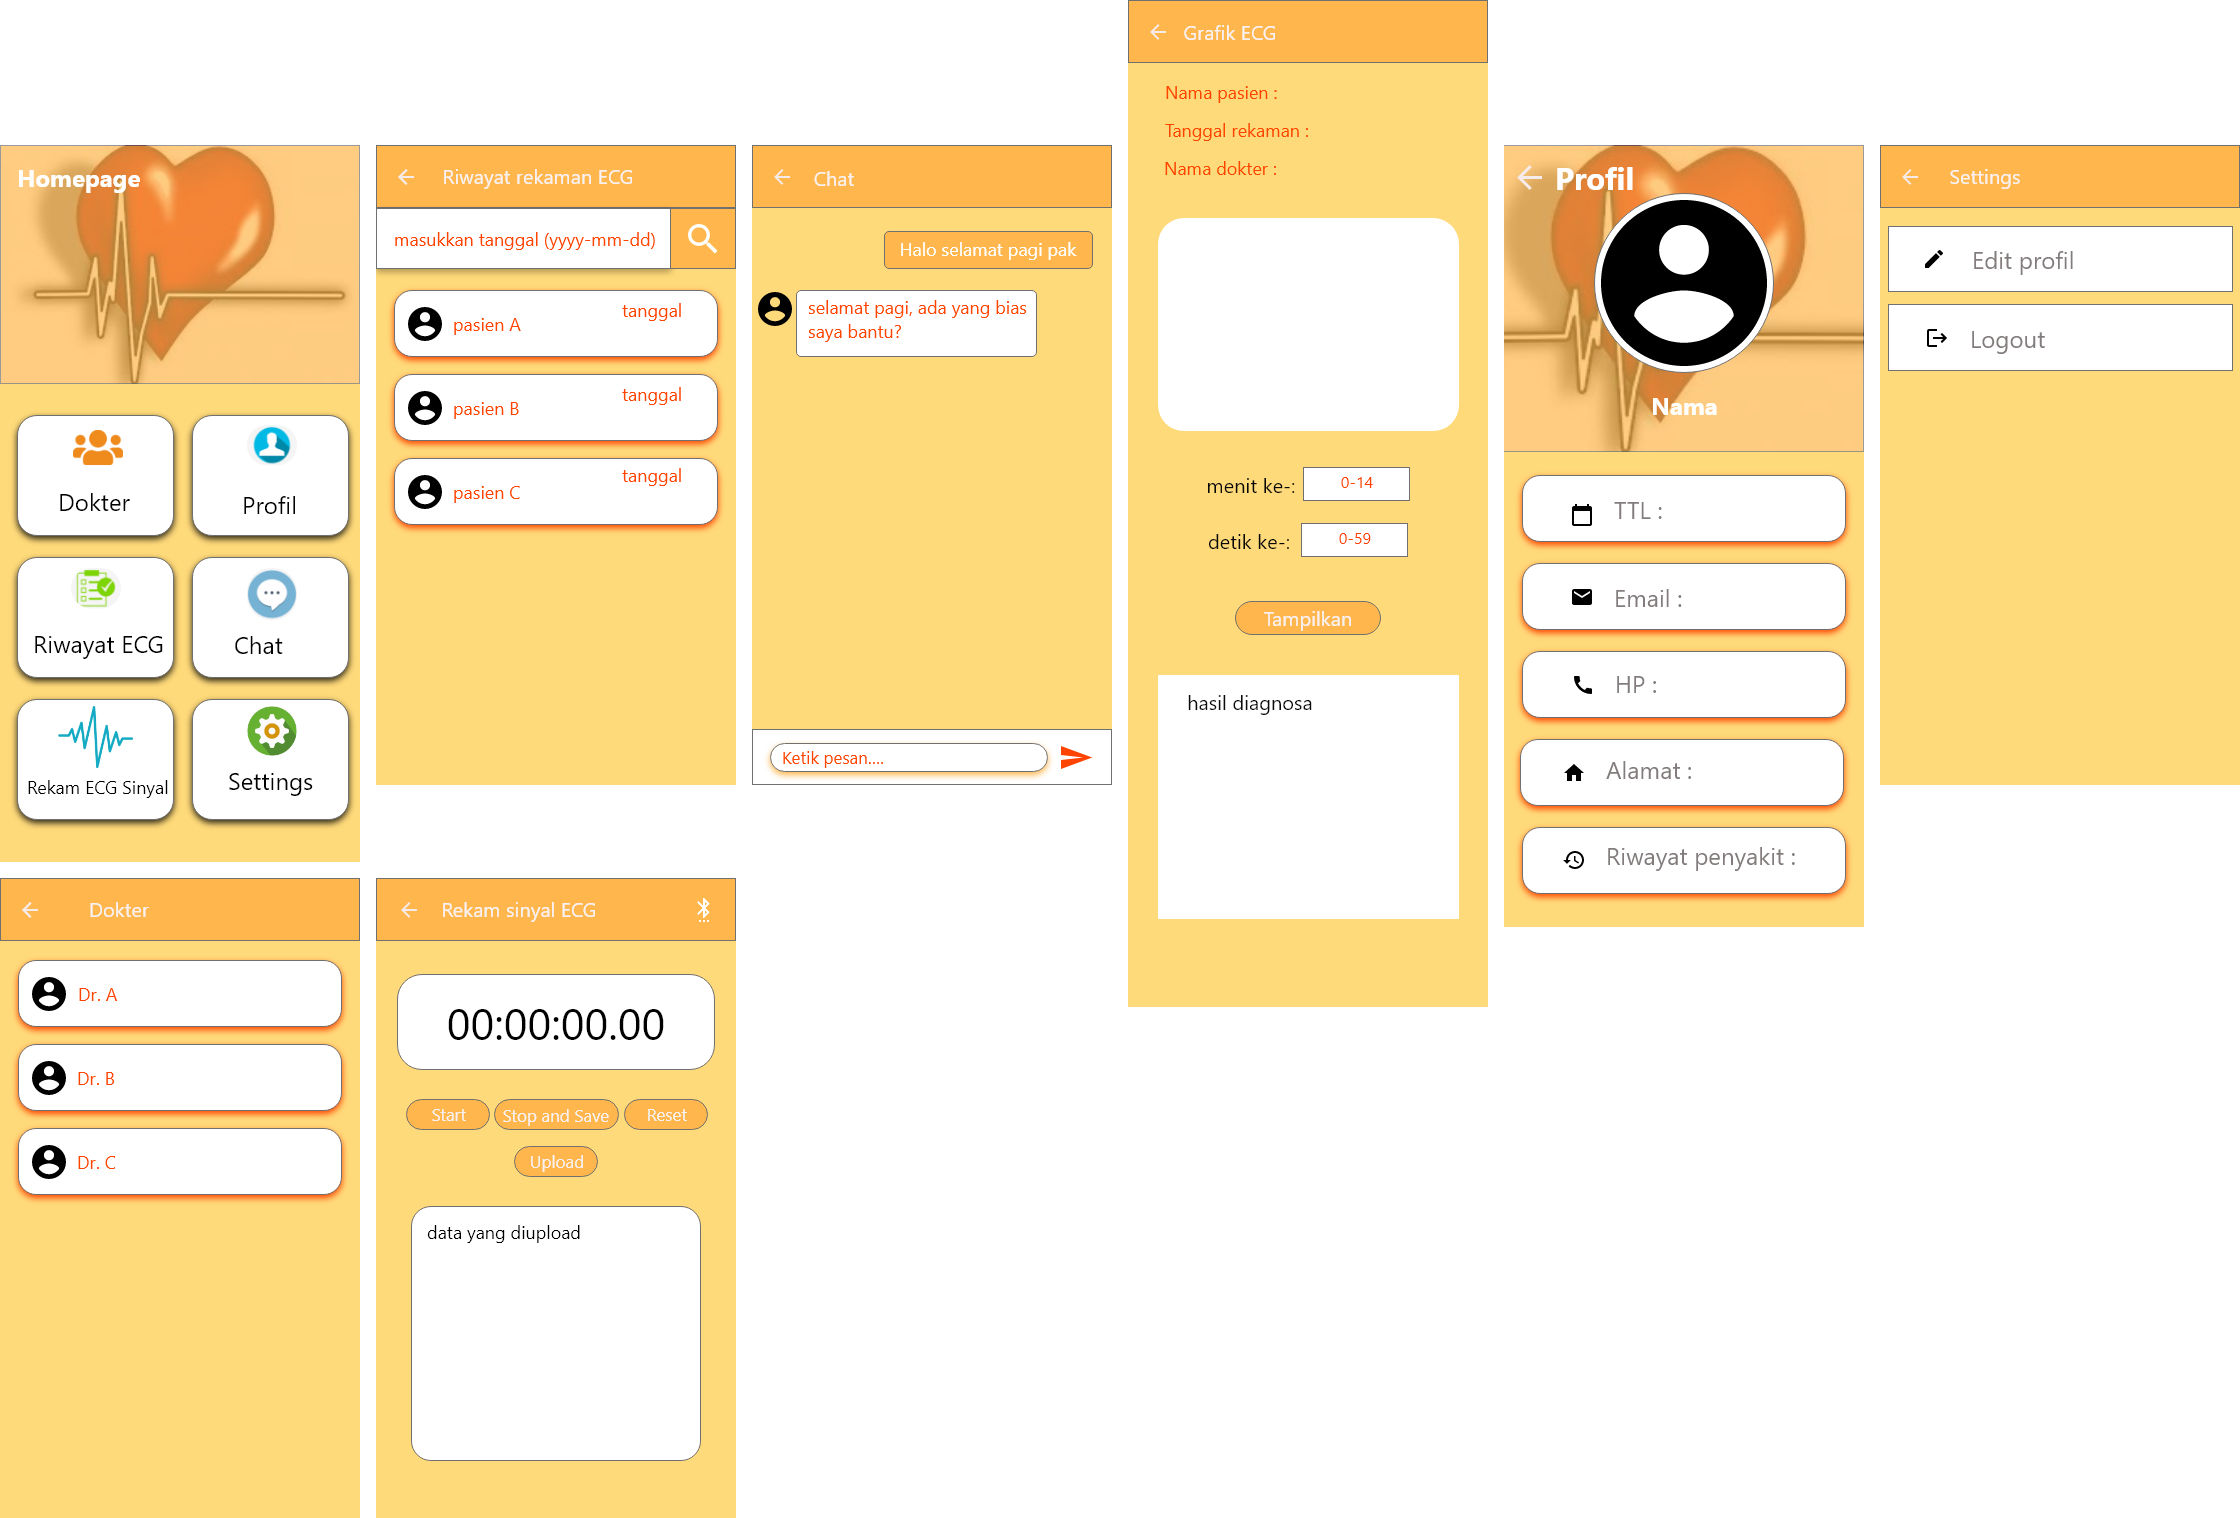
\includegraphics[width=1\textwidth]{img/pasienUI.png}
	\caption{Desain UI pada aplikasi pasien.}
	\label{fig:3.3}
\end{figure}
\vspace{1ex}
Dapat diketahui dari desai UI pasien tersebut terdapat 8 screen, yaitu:
\begin{enumerate}
	\vspace{-2mm}
	\item Homepage screen, yang mana merupakan halaman utaman pada aplikasi. Pada Homepage screen dokter tersedia 6 buah menu yaitu Dokter untuk berpindah menuju halaman daftar dokter yang ada, Profil untuk berpindah ke halaman profil, Chat untuk berpindah ke halaman chat, Riwayat ECG untuk berpindah halaman menuju riwayat rekaman ECG, Rekam ECG Sinyal untuk berpindah menuju halaman perekaman data ECG, dan Settings untuk berpindah ke halaman settings,
	\vspace{-2mm}
	\item Riwayat rekaman ECG screen yang sama seperti screen dokter, pada halaman ini pasien juga dapat mencari riwayat rekaman ECG pada waktu tertentu sesuai yang telah diinputkan,
	\vspace{-2mm}
	\item Chat screen, desain halaman chat untuk pasien juga sama seperti dokter,
	\vspace{-2mm}
	\item Grafik ECG screen, sama seperti dokter, pasien juga dapat melihat grafik ECG miliknya yang telah direkam. Pasien juga dapat melihat grafik pada menit dan detik tertentu. Pada halaman ini pasien juga dapat melihat hasil diagnosa yang telah ditambahkan oleh dokter,
	\vspace{-2mm}
	\item Profil screen, desain halaman profil untuk pasien juga sama seperti dokter. Pada halaman ini menampilkan informasi pasien yaitu foto, nama lengkap, tanggal lahir, email, nomor telepon, dan alamat,
	\vspace{-2mm}
	\item Settings screen, yang mana merupakan halaman yang berisi menu untuk mengubah informasi pada halaman profil dan juga terdapat menu \textit{logout} untuk keluar dari aplikasi.
	\vspace{-2mm}
	\item Dokter screen, yang mana merupakan menu tambahan untuk pasien. Pada halaman ini pasien dapat melihat daftar dokter yang ada dan melihat informasi profil dokter.
	\vspace{-2mm}
	\item Rekam sinyal ECG screen, yang mana merupakan halaman yang khusus untuk pasien. Pada halaman ini pasien dapat melakukan perekaman data ECG yang dikirim oleh arduino melalui bluetooth HC-05. Pada halaman ini terdapat icon bluetooth pada top bar yang mana berfungsi untuk menghubungkan bluetooth smartphone dengan modul HC-05. Halaman ini memiliki desain seperti stopwatch yang memiliki tombol start, stop, dan reset. Tombol start untuk memulai rekaman, stop untuk menghentikan rekaman sekaligus menyimpan data kedalam file.txt sementara, reset untuk mengembalikan ulang waktu stopwatch, dan terdapat tombol upload untuk mengupload data ke dalam database, data yang diupload dapat dilihat pada layar dibawahnya.
\end{enumerate}
\vspace{1ex}

Pada kedua gambar tersebut terdapat
sedikit perbedaan desain antara milik dokter dengan pasien. Perbedaan pertama desain tersebut terdapat pada jumlah menu di homepage. Pada desain UI homepage milik dokter memiliki menu yang lebih sedikit daripada pasien, hal ini dikarenakan dokter tidak perlu menggunakan fitur rekam sinyal sinyal dan juga fitur melihat dokter lain. Perbedaan kedua terdapat
pada layar grafik ECG yang berguna dapat menampilkan grafik sinyal jantung pada menit dan detik tertentu sesuai keinginan user.
Perbedaan pada layar grafik ECG adalah pada layar dokter
terdapat form dan tombol untuk menambahkan diagnosa sedangkan pada layar pasien hanya membutuhkan hasil diagnosa.

\vspace{1ex}

\section{Desain Database}
\vspace{1ex}

Pada penelitian ini menggunakan database MySQL. Berikut merupakan desain database pada penelitian ini ditunjukkan pada Gambar \ref{fig:3.4}. 
\begin{figure}[H] \centering
	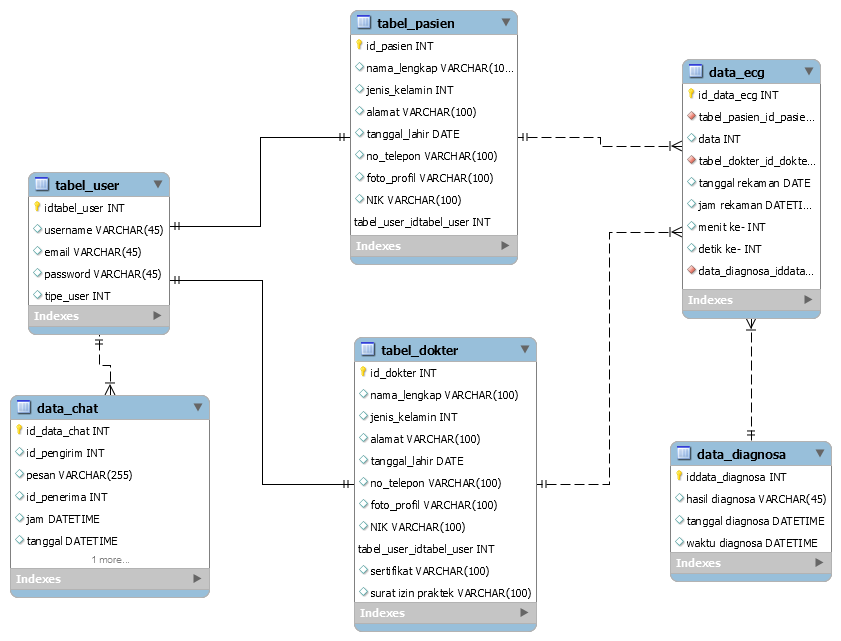
\includegraphics[width=1\textwidth]{img/db_revv.png}
	\caption{Desain database.}
	\label{fig:3.4}
\end{figure}
\vspace{1ex}

Dalam database terdapat 6 tabel yang diperlukan untuk menyimpan masing-masing data, yaitu:
\begin{enumerate}[nolistsep]
	\item Tabel tabel\_user, memiliki 5 kolom. Tabel user digunakan sebagai tempat menyimpan data login pengguna aplikasi yaitu username, email, password, dan tipe user untuk lebih mudah membedakan antara data pasien dan dokter. Tabel user memiliki relasi dengan 3 tabel lainnya yaitu tabel pasien, tabel dokter, dan tabel data \textit{chat}.
	\item Tabel tabel\_pasien, memiliki 9 kolom dengan 1 kolom merupakan \textit{foreign key} dari tabel user. Tabel pasien digunakan sebagai tempat menyimpan data pasien berupa id pasien, nama lengkap, jenis kelamin, alamat, tanggal lahir, NIK, nomor telepon, foto profil , dan id user yang merupakan \textit{foreign key} dari tabel user. Tabel pasien memiliki 2 relasi dengan 2 tabel lainnya yaitu tabel user dan tabel data ECG.
	\item Tabel tabel\_dokter, memiliki 11 kolom  dengan 1 kolom merupakan \textit{foreign key} dari tabel user. Tabel dokter digunakan sebagai tempat menyimpan data dokter berupa id dokter, nama lengkap, jenis kelamin, alamat, tanggal lahir, NIK, nomor telepon, foto profil, sertifikat, surat izin praktek, dan id user yang merupakan \textit{foreign key} dari tabel user. Tabel dokter memiliki 2 relasi dengan 2 tabel lainnya yaitu tabel user dan tabel data ECG.  
	\item Tabel data\_ecg, memiliki 9 kolom, 3 kolom merupakan foreign key dari tabel pasien, tabel dokter, dan tabel data\_diagnosa. Tabel data\_ecg digunakan untuk menyimpan data rekaman sinyal jantung pasien yang mana akan dapat ditampilkan pada aplikasi android. Tabel data ECG terdiri dari kolom id\_data\_ecg, id\_pasien yang merupakan \textit{foreign key} dari tabel\_pasien, data, id\_dokter yang merupakan \textit{foreign key} dari tabel\_dokter, tanggal rekaman, jam rekaman, jam, menit, detik, dan id\_data\_diagnosa yang merupakan \textit{foreign key} dari tabel data diagnosa.
	\item Tabel data\_diagnosa, memiliki 4 kolom, Tabel ini digunakan sebagai tempat penyimpanan hasil diagnosa yang telah ditambahkan oleh dokter. Tabel data diagnosa memiliki relasi dengan tabel data ecg. Tabel ini terdiri dari kolom id\_data\_diagnosa, hasil diagnosa, tanggal diagnosa, dan waktu diagnosa.		
	\item Dan tabel data\_chat yang memiliki 6 kolom. Tabel data\_chat diperlukan untuk menyimpan data chat antara pasien dan dokter. Tabel ini terdiri dari kolom id\_data\_chat, id\_pengirim, pesan, id\_penerima, jam, dan tanggal. Tabel data\_chat memiliki relasi dengan tabel tabel\_user.
\end{enumerate}

\section{Akuisisi Data}
\vspace{1ex}

Akuisisi data pada penelitian ini menggunakan sensor ECG AD8232. Setelah sensor AD8232 membaca sinyal jantung pasien, kemudian data sinyal jantung akan diproses pada mikrokontroler arduino. Setelah data sinyal diproses oleh arduino, data sinyal akan dikirimkan melalui serial bluetooth HC-05. \textit{Baudrate} yang digunakan pada modul bluetooth HC-05 adalah 57600. Data sinyal ECG yang dikirimkan pada aplikasi android akan disimpan sementara pada file.txt. Akuisisi data yang dilakukan pada penelitian ini adalah sebesar kurang lebih 128 Hz atau 128 data sampel sinyal tiap detik. Berikut merupakan perangkat ECG yang digunakan, ditunjukkan pada gambar \ref{fig:3.4.1}.
\begin{figure}[H] \centering
	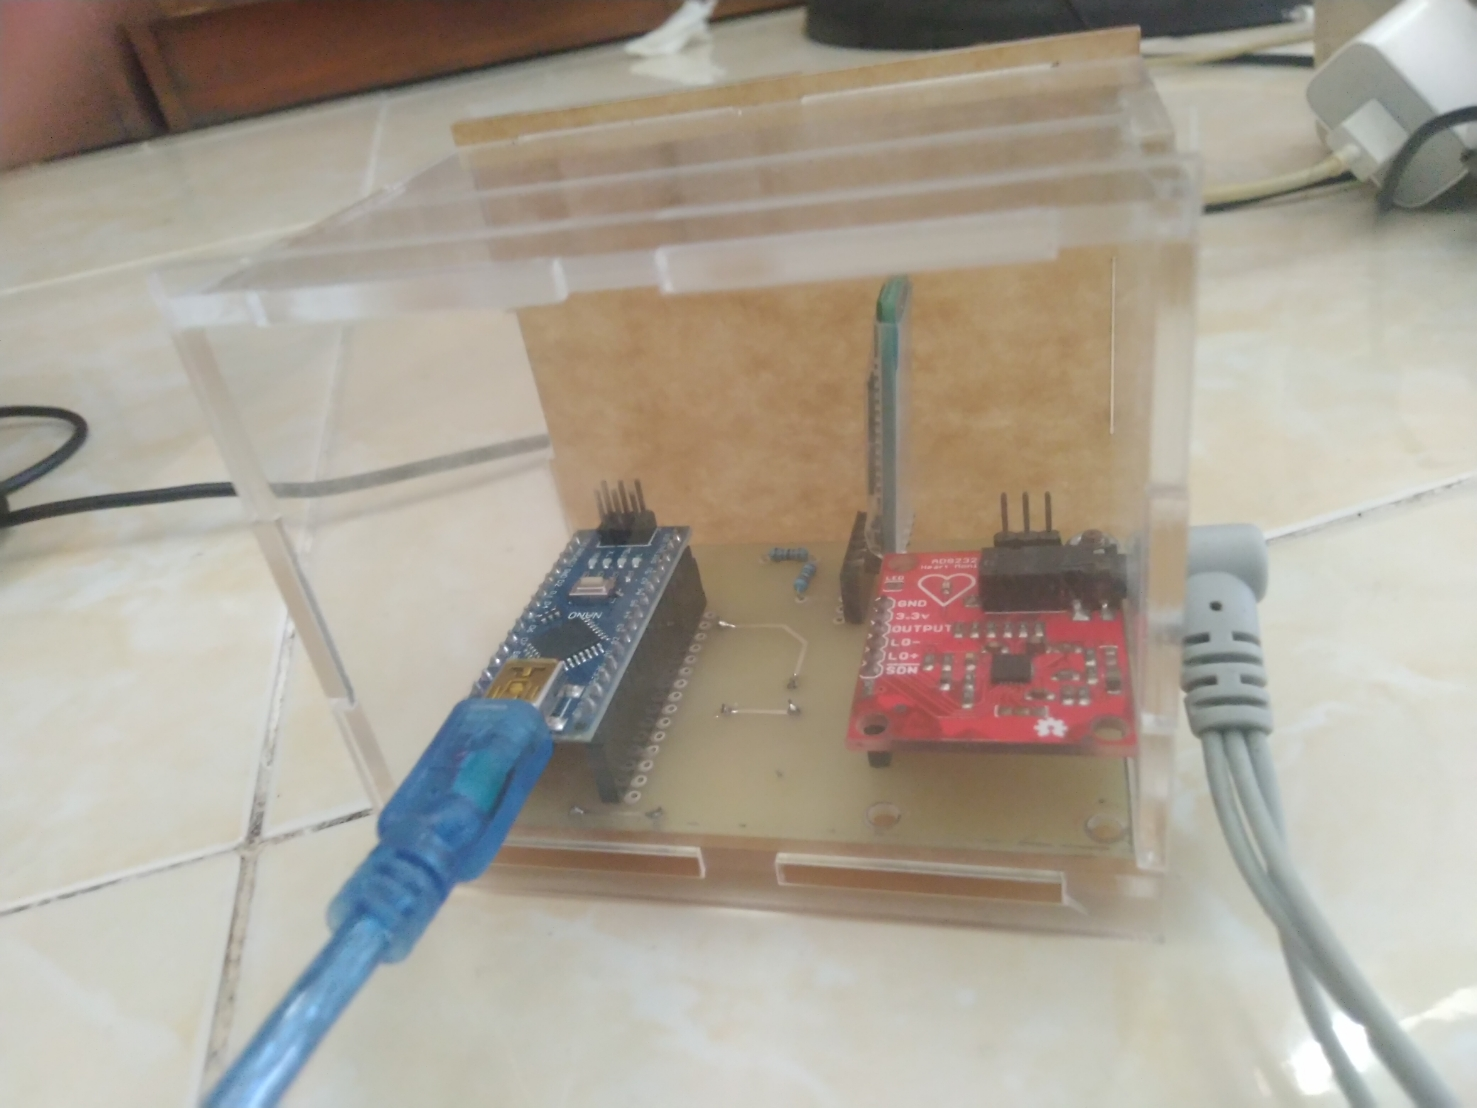
\includegraphics[width=0.6\textwidth]{img/fotoperangkat1.jpg}
	\caption{Perangkat ECG.}
	\label{fig:3.4.1}
\end{figure}
\vspace{1ex}

Mekanisme kerja pada akuisisi data adalah modul Bluetooth menunggu perintah dari aplikasi, kemudian aplikasi memberi perintah angka "1" yang mana berarti meminta alat mulai mengambil data. Disaat arduino menerima perintah "1" dari HC-05, arduino mulai melakukan looping mengambil data dari sensor AD8232. Apabila waktu rekaman sudah berjalan selama 15 menit, aplikasi akan mengirim perintah angka "0" pada HC-05 yang mana berarti untuk menghentikan rekaman. Pada saat arduino menerima perintah "0" dari HC-05, maka arduino akan berhenti melakukan looping untuk mengambil data. Berikut merupakan gambar diagram mekanisme kerja akuisisi data Gambar \ref{fig:3.4.2}.
\begin{figure}[H] \centering
	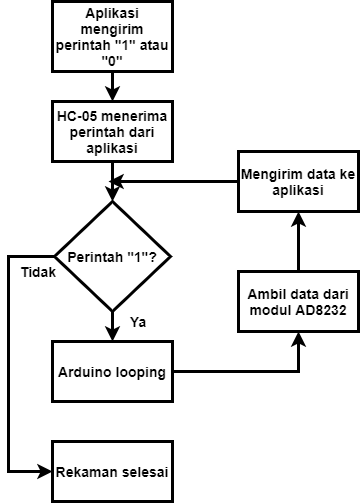
\includegraphics[width=0.6\textwidth]{img/diagramAkuisisi.png}
	\caption{Diagram mekanisme akuisisi data.}
	\label{fig:3.4.2}
\end{figure}


\section{Perekaman Data}
\vspace{1ex}
Perekaman data dilakukan oleh aplikasi android. Proses rekaman pada pasien adalam kurang dari sampai dengan 15 menit. Berikut merupakan implementasi halaman rekaman data pada aplikasi android ditunjukkan oleh Gambar \ref{fig:3.5}.

\begin{figure}[H] \centering
	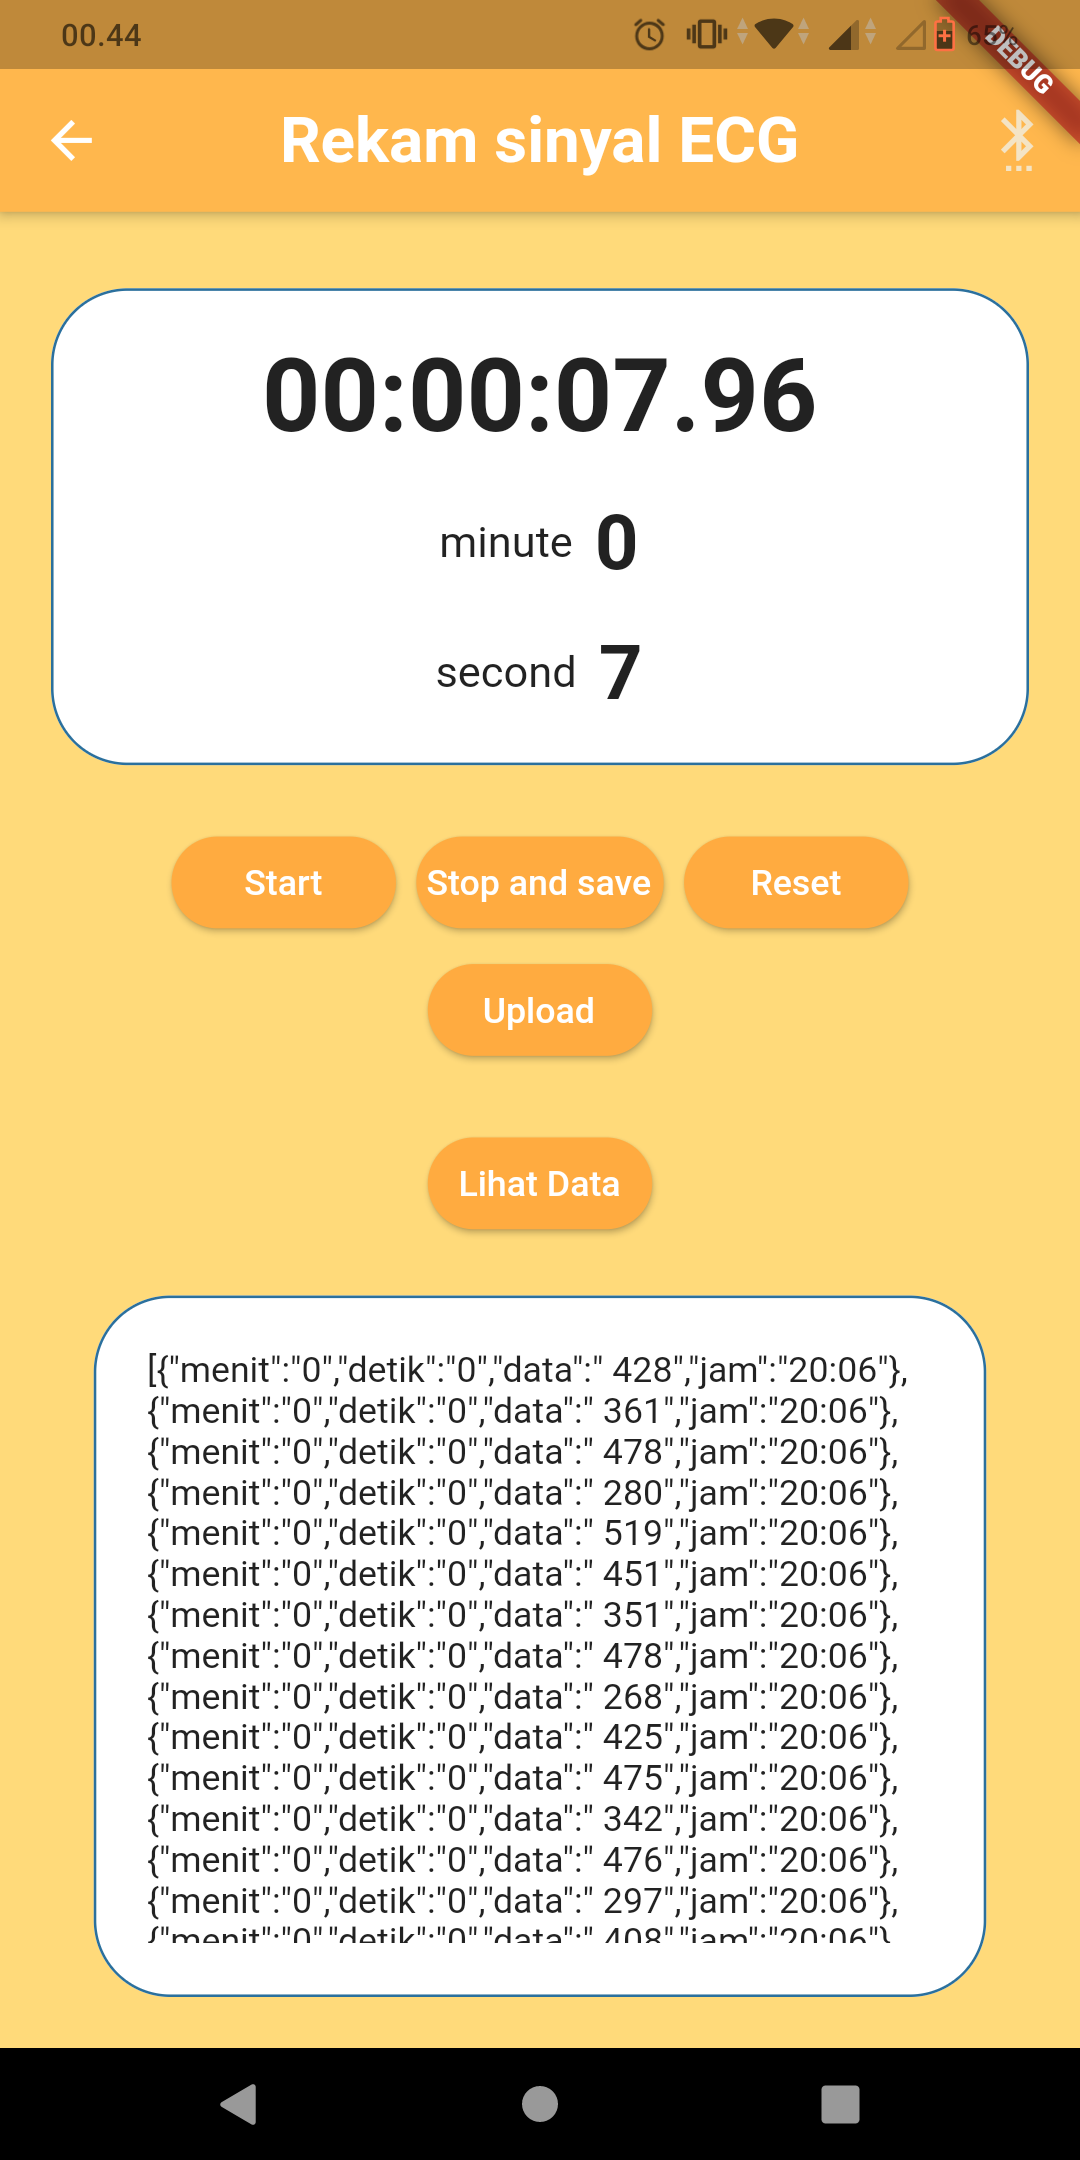
\includegraphics[width=0.37\textwidth]{img/layar_rekaman.png}
	\caption{Implementasi UI Rekam Sinyal ECG.}
	\label{fig:3.5}
\end{figure}


Selama proses rekaman berlangsung, aplikasi akan menerima data sinyal terus-menerus dari modul bluetooth HC-05. Aplikasi akan menyimpan data sinyal kedalam string saat proses rekaman berlangsung. Setelah rekaman selesai, aplikasi akan menyimpan data sinyal dari variabel string kedalam file.txt. Dapat dilihat pada layar rekaman (Gambar \ref{fig:3.5}) terdapat stopwatch untuk mengetahui seberapa lama telah melakukan rekaman. Pada layar ini terdapat 4 tombol, yaitu tombol Start yang berfungsi untuk memulai rekaman, Stop and Save berfungsi untuk menghentikan rekaman dan menyimpan data dalam file.txt, tombol Reset berfungsi untuk mengembalikan stopwatch dengan keadaan waktu 00:00:00.00, tombol Upload yang berguna untuk mengupload data sinyal menuju database, dan yang terakhir adalah tombol Lihat Data yang berguna untuk menampilkan isi dari file.txt. Isi file.txt ditampilkan pada box putih seperti yang tertera dibawah tomboh Lihat Data.

\vspace{1ex} 
\section{Penyimpanan Data}
\vspace{1ex}
Data rekaman sinyal  ECG yang diupload oleh aplikasi pada database disimpan dalam tabel data\_ecg. Data ECG disimpan beserta atribut lainnya sesuai kolom yang ada pada tabel data\_ecg. Rincian kolom tersebut sebagai berikut:
\begin{enumerate}
	\vspace{-2mm}
	\item Kolom id\_data\_ecg dengan tipe data BIGINT sebagai primary key dan auto increment untuk menyimpan nomor urut data ECG yang didapat,
	\vspace{-2mm}
	\item Kolom id\_pasien dengan tipe data INT untuk menyimpan id pasien,
	\vspace{-2mm}
	\item Kolom data dengan tipe data INT berguna untuk menyimpan data ECG hasil rekaman,
	\vspace{-2mm}
	\item Kolom menit dengan tipe data INT untuk menyimpan waktu menit,
	\vspace{-2mm}
	\item Kolom detik dengan tipe data INT untuk menyimpan waktu detik,
	\vspace{-2mm}
	\item Kolom id\_dokter dengan tipe data INT untuk menyimpan id dokter,
	\vspace{-2mm}
	\item Kolom tanggal dengan tipe data DATE berguna untuk menyimpan data tanggal rekaman,
	\vspace{-2mm}
	\item Kolom jam dengan tipe data VARCHAR untuk menyimpan nomor sample data pada waktu mulai rekaman sampai akhir rekaman, (data ini digunakan sebagai sumbu X untuk menggambarkan grafik pada aplikasi),
	\vspace{-2mm}
	\item Kolom channel dengan tipe data INT berfungsi untuk menyimpan channel lead ECG,
	\vspace{-2mm}
	\item Kolom clock dengan tipe data VARCHAR untuk menyimpan waktu mulai rekaman,
	\vspace{-2mm}
	\item Kolom id\_data\_diagnosa dengan tipe data INT untuk menyimpan nomor id diagnosa dari tabel data\_diagnosa,
\end{enumerate}

Berikut merupakan potongan database pada tabel data\_ecg yang ditunjukkan pada Gambar  \ref{fig:3.6}.

\begin{figure}[H] \centering
	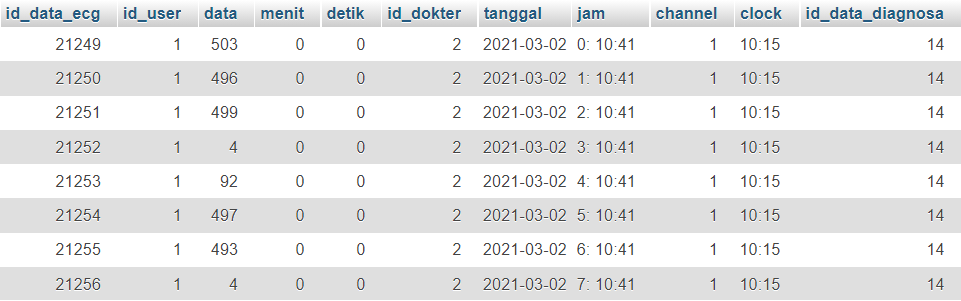
\includegraphics[width=1\textwidth]{img/tabel data ecg.png}
	\caption{Tabel data\_ecg.}
	\label{fig:3.6}
\end{figure}

\vspace{1ex} 
\section{Menampilkan Data}
\vspace{1ex}

Data yang telah disimpan pada database yaitu dalam tabel data\_ecg dapat diambil oleh aplikasi dokter dan pasien untuk ditampilkan dalam bentuk grafik. Pada screen grafik ECG, pengguna dapat melihat data ECG sesuai dengan waktu yang ditentukan yaitu pada (menit awal, detik awal) sampai dengan (menit akhir, detik akhir) dengan selisih waktu detik yang dapat diatur pada box (parameter range). Pengguna juga dapat melihat data selanjutnya dengan menekan tombol "selanjutnya" serta dapat kembali ke data sebelumnya dengan menakan tombol "sebelumnya". Berikut adalah tampilan dari screen Grafik sinyal ECG dokter ditunjukkan pada Gambar \ref{fig:3.7}. 

\begin{figure}[H] \centering
	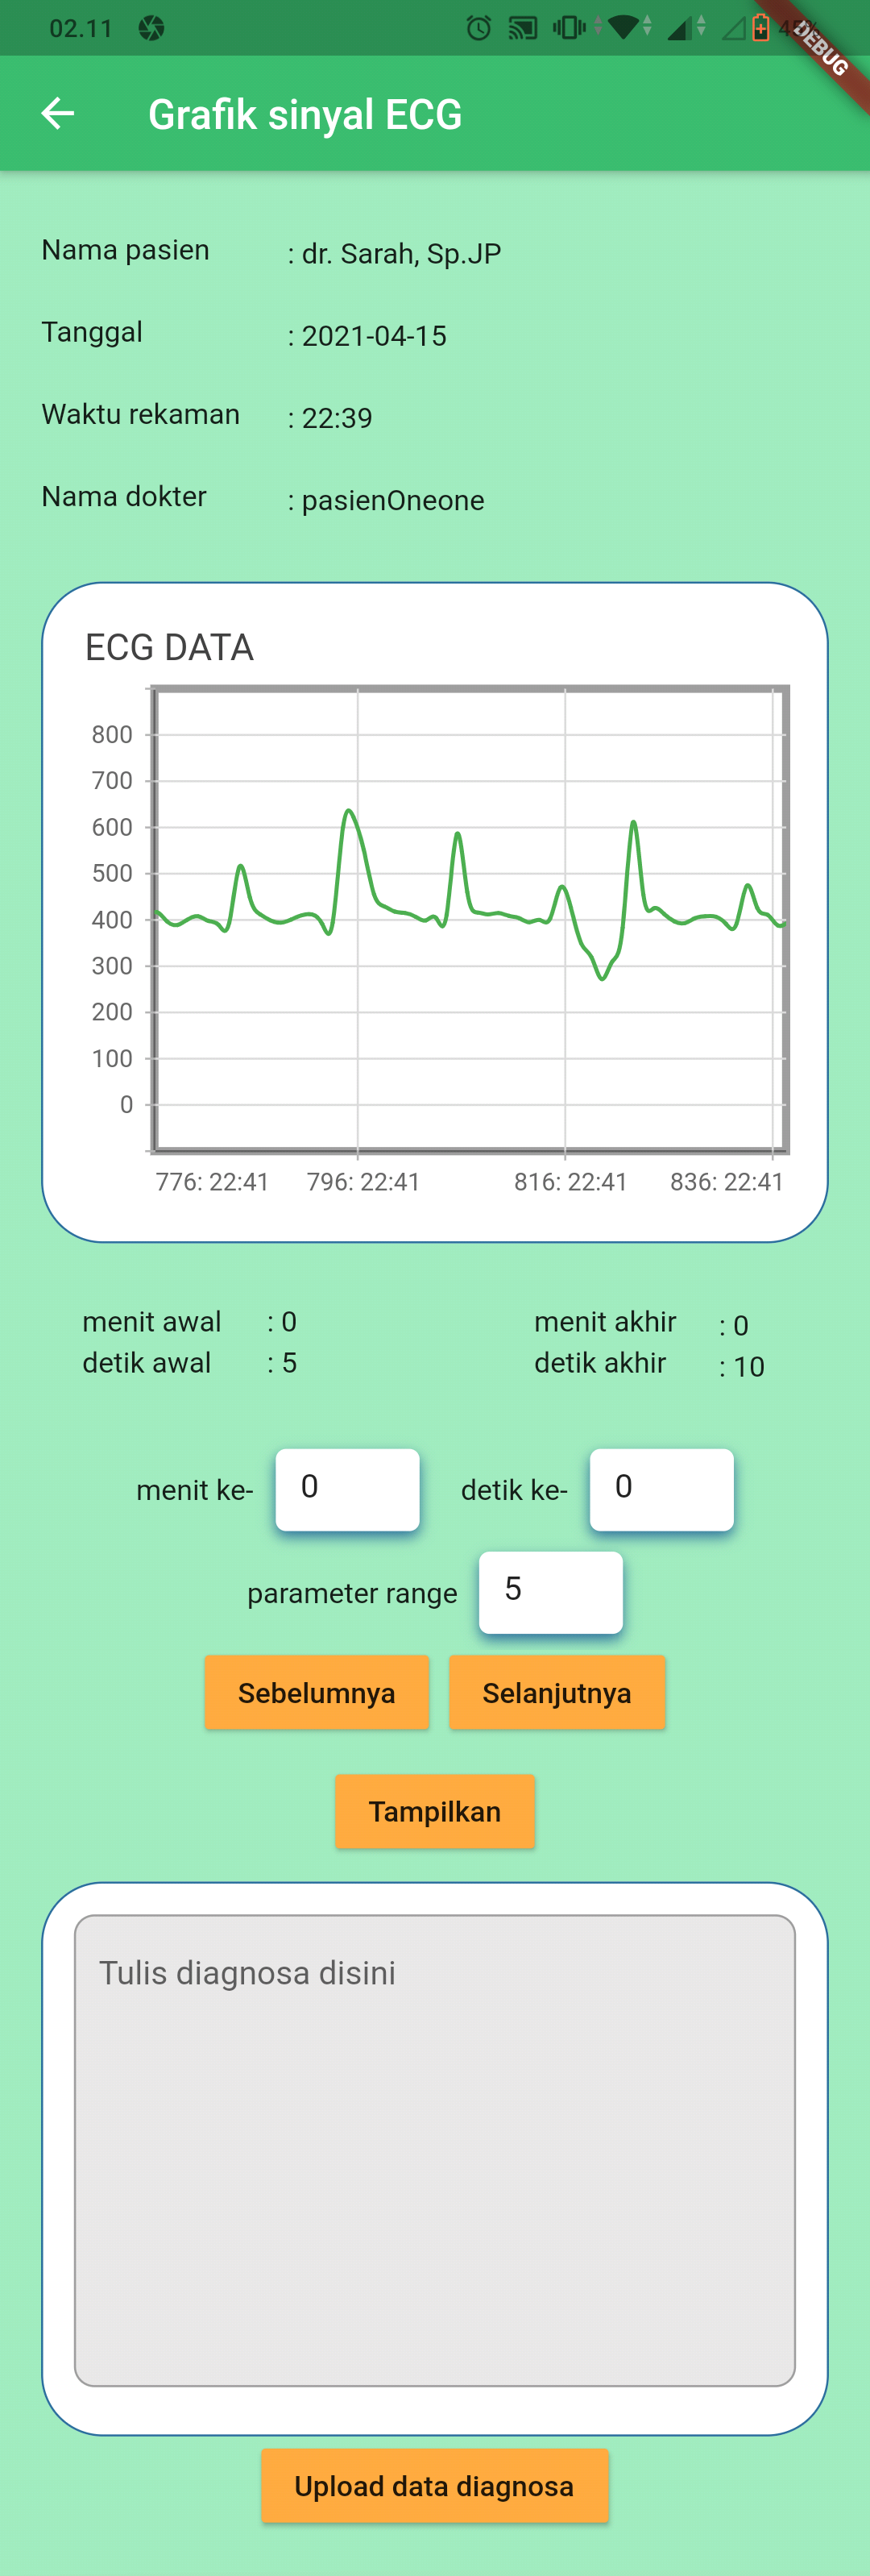
\includegraphics[width=0.4\textwidth]{img/layar_grafikECGdokter.png}
	\caption{Implementasi UI Grafik ECG dokter.}
	\label{fig:3.7}
\end{figure}

Pada grafik tersebut terdiri dari sumbu X dan sumbu Y. Sumbu X merupakan data ECG yang diambil dari kolom data pada tabel data\_ecg, sedangkan sumbu Y merupakan data dari kolom jam pada tabel data\_ecg (Gambar \ref{fig:3.6}). Untuk tampilan Grafik sinyal ECG pasien tidak jauh berbeda. Berikut adalah tampilan dari screen Grafik sinyal ECG pasien ditunjukkan pada Gambar \ref{fig:3.8}.

\begin{figure}[H] \centering
	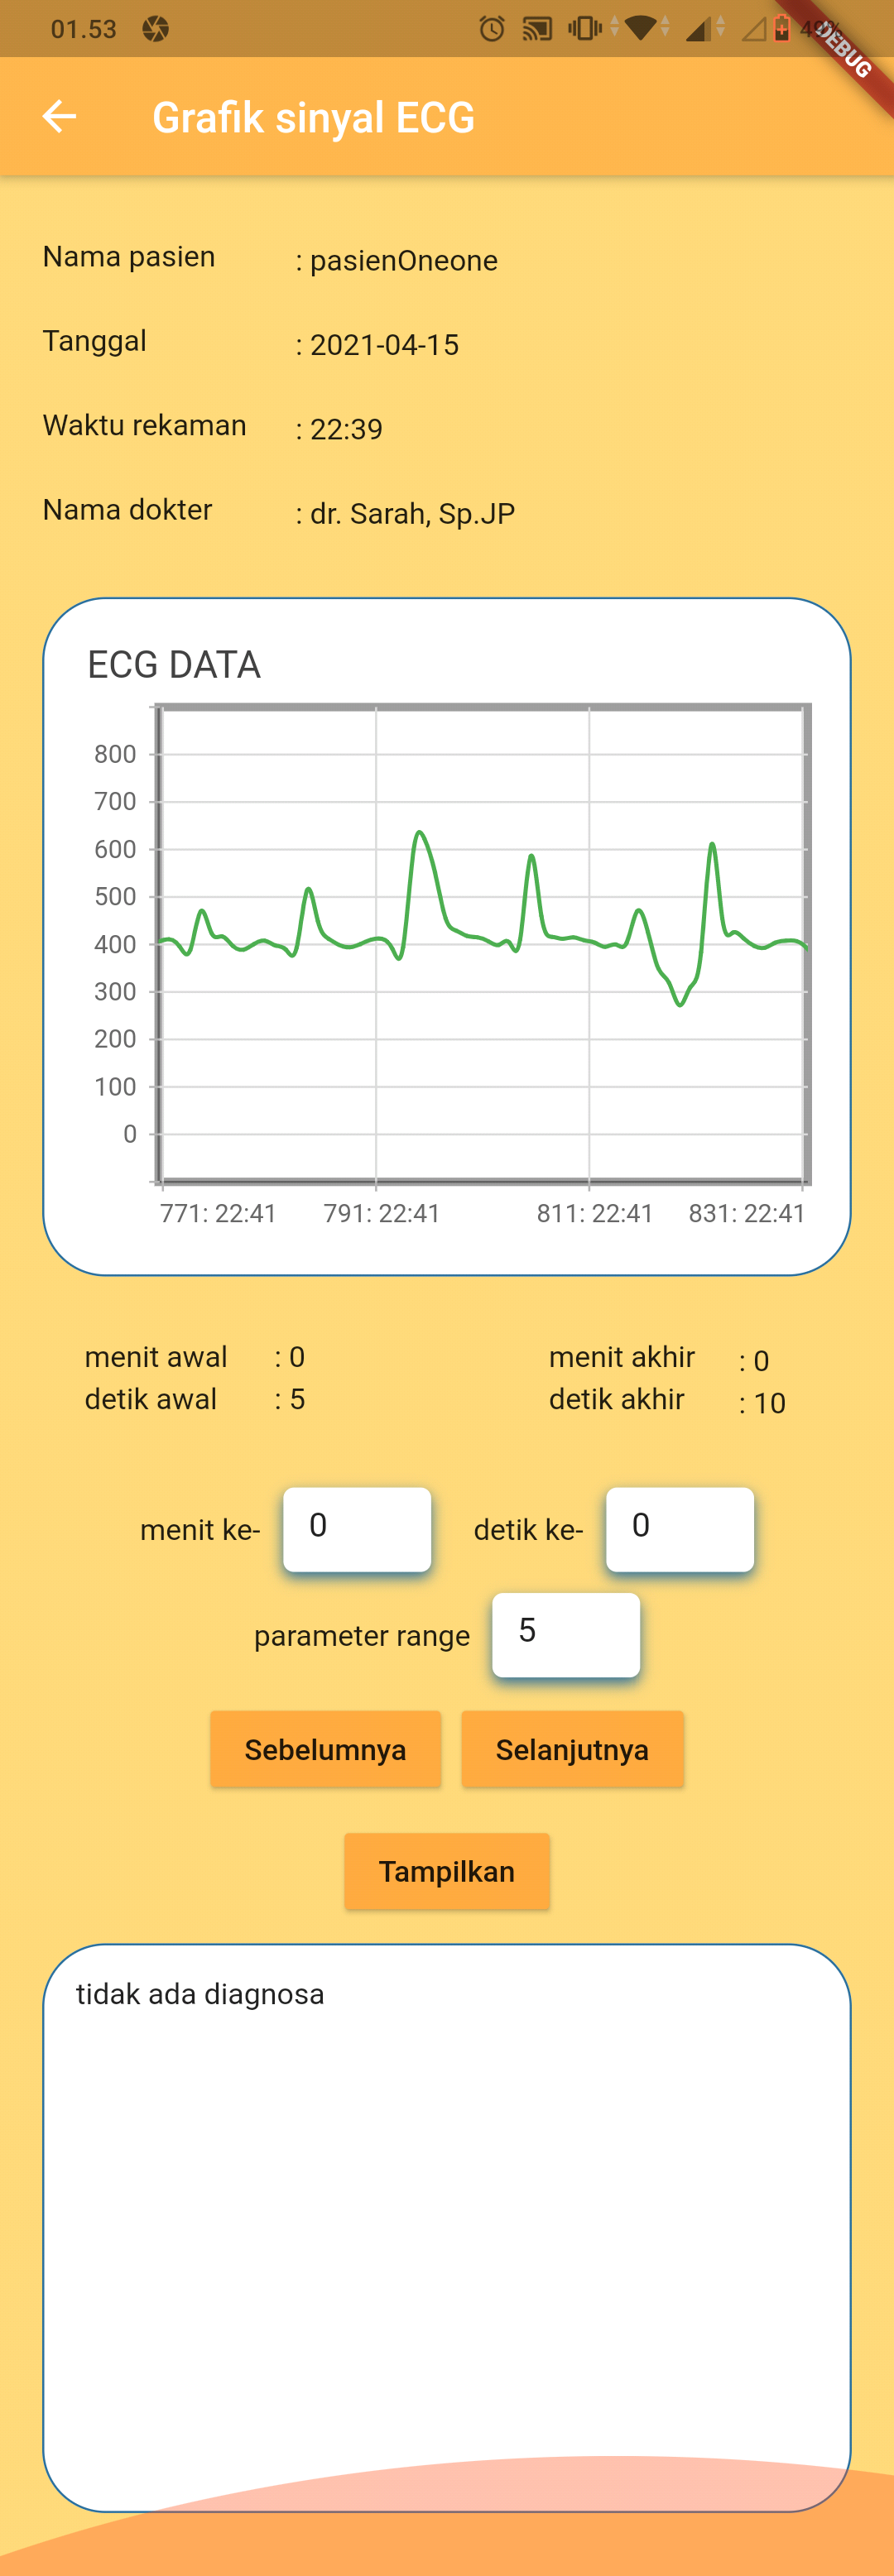
\includegraphics[width=0.4\textwidth]{img/layar_grafikECGpasien.png}
	\caption{Implementasi UI Grafik ECG pasien.}
	\label{fig:3.8}
\end{figure}

Dapat dilihat pada screen dokter (Gambar \ref{fig:3.7}) terdapat box berwarna abu-abu dengan keterangan "Tulis diagnosa disini" yang berarti pada screen dokter dapat ditambahkan diagnosa melalui box tersebut dan kemudian diupload dengan cara menekan tombol "Upload data diagnosa". Sedang kan pada screen pasien (Gambar \ref{fig:3.8}) hanya terdapat box putih tanpa ada tombol upload data diagnosa. Box putih tersebut adalah tempat hasil diagnosa yang diberikan oleh dokter.

\vspace{1ex} 
\section{Diagnosa Data}
\vspace{1ex}

Diagnosa sinyal ECG dilakukan secara manual yaitu oleh dokter. Dokter dapat menambahkan diagnosa pada rekaman ECG pasien dimenit dan detik tertentu, dapat dilihat pada Gambar \ref{fig:3.7} sebelumnya. Pada screen tersebut terdapat box untuk dokter yang berfungsi untuk tempat menambahkan diagnosa. Setelah dokter selesai menambahkan diagnosa, kemudian dapat mengupload ke database melalui tombol "Upload data diagnosa". Diagnosa yang telah diupload ke database akan disimpan pada tabel data\_diagnosa. Kemudian data diagnosa dapat ditampilkan pada aplikasi smarftphone pasien seperti yang ditunjukkan Gambar \ref{fig:3.9}.

\begin{figure}[H] \centering
	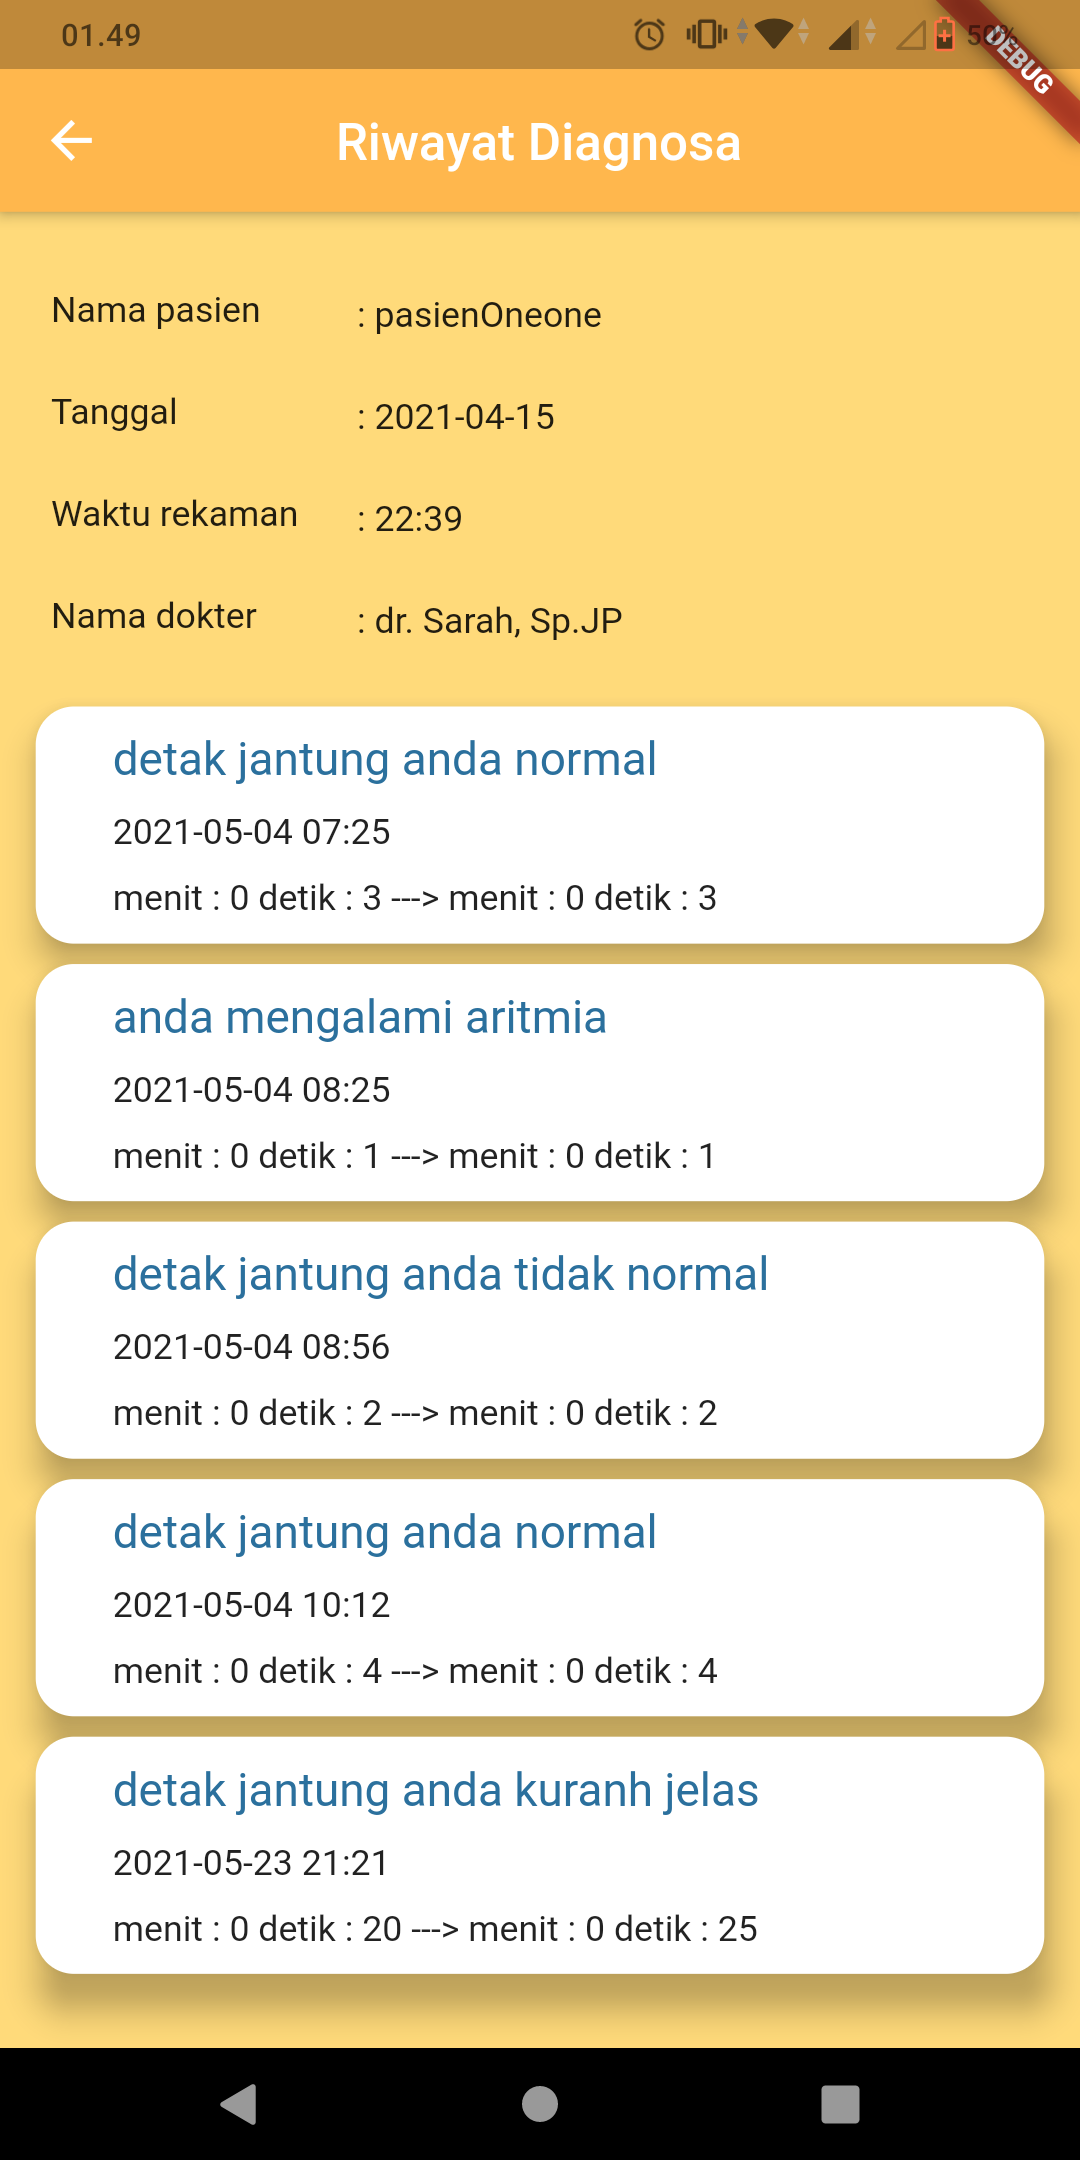
\includegraphics[width=0.4\textwidth]{img/layar_riwayatdiagnosa.png}
	\caption{Implementasi UI Riwayat Diagnosa.}
	\label{fig:3.9}
\end{figure}

\vspace{1ex}
\section{Fitur Chat}
\vspace{1ex}

Pada aplikasi ini tersedia fitur chat agar pasien dapat berkonsultasi dengan dokter spesialis. Untuk cara kerja pada screen chat ini, aplikasi akan melakukan refresh setiap detik dan akan mengambil data dari database yaitu pada tabel data\_chat agar pesan terbaru pada screen chat dapat muncul. Saat mengirim pesan, pesan dari kedua user pasangan chat akan diupload pada tabel yang sama. Untuk membedakannya terdapat pada kolom id\_pengirim dan id\_penerima yang terdapat pada tabel data\_chat (Gambar \ref{fig:3.6}). Tampilan screen chat pasien dapat dilihat pada Gambar \ref{fig:3.10}.

\begin{figure}[H] \centering
	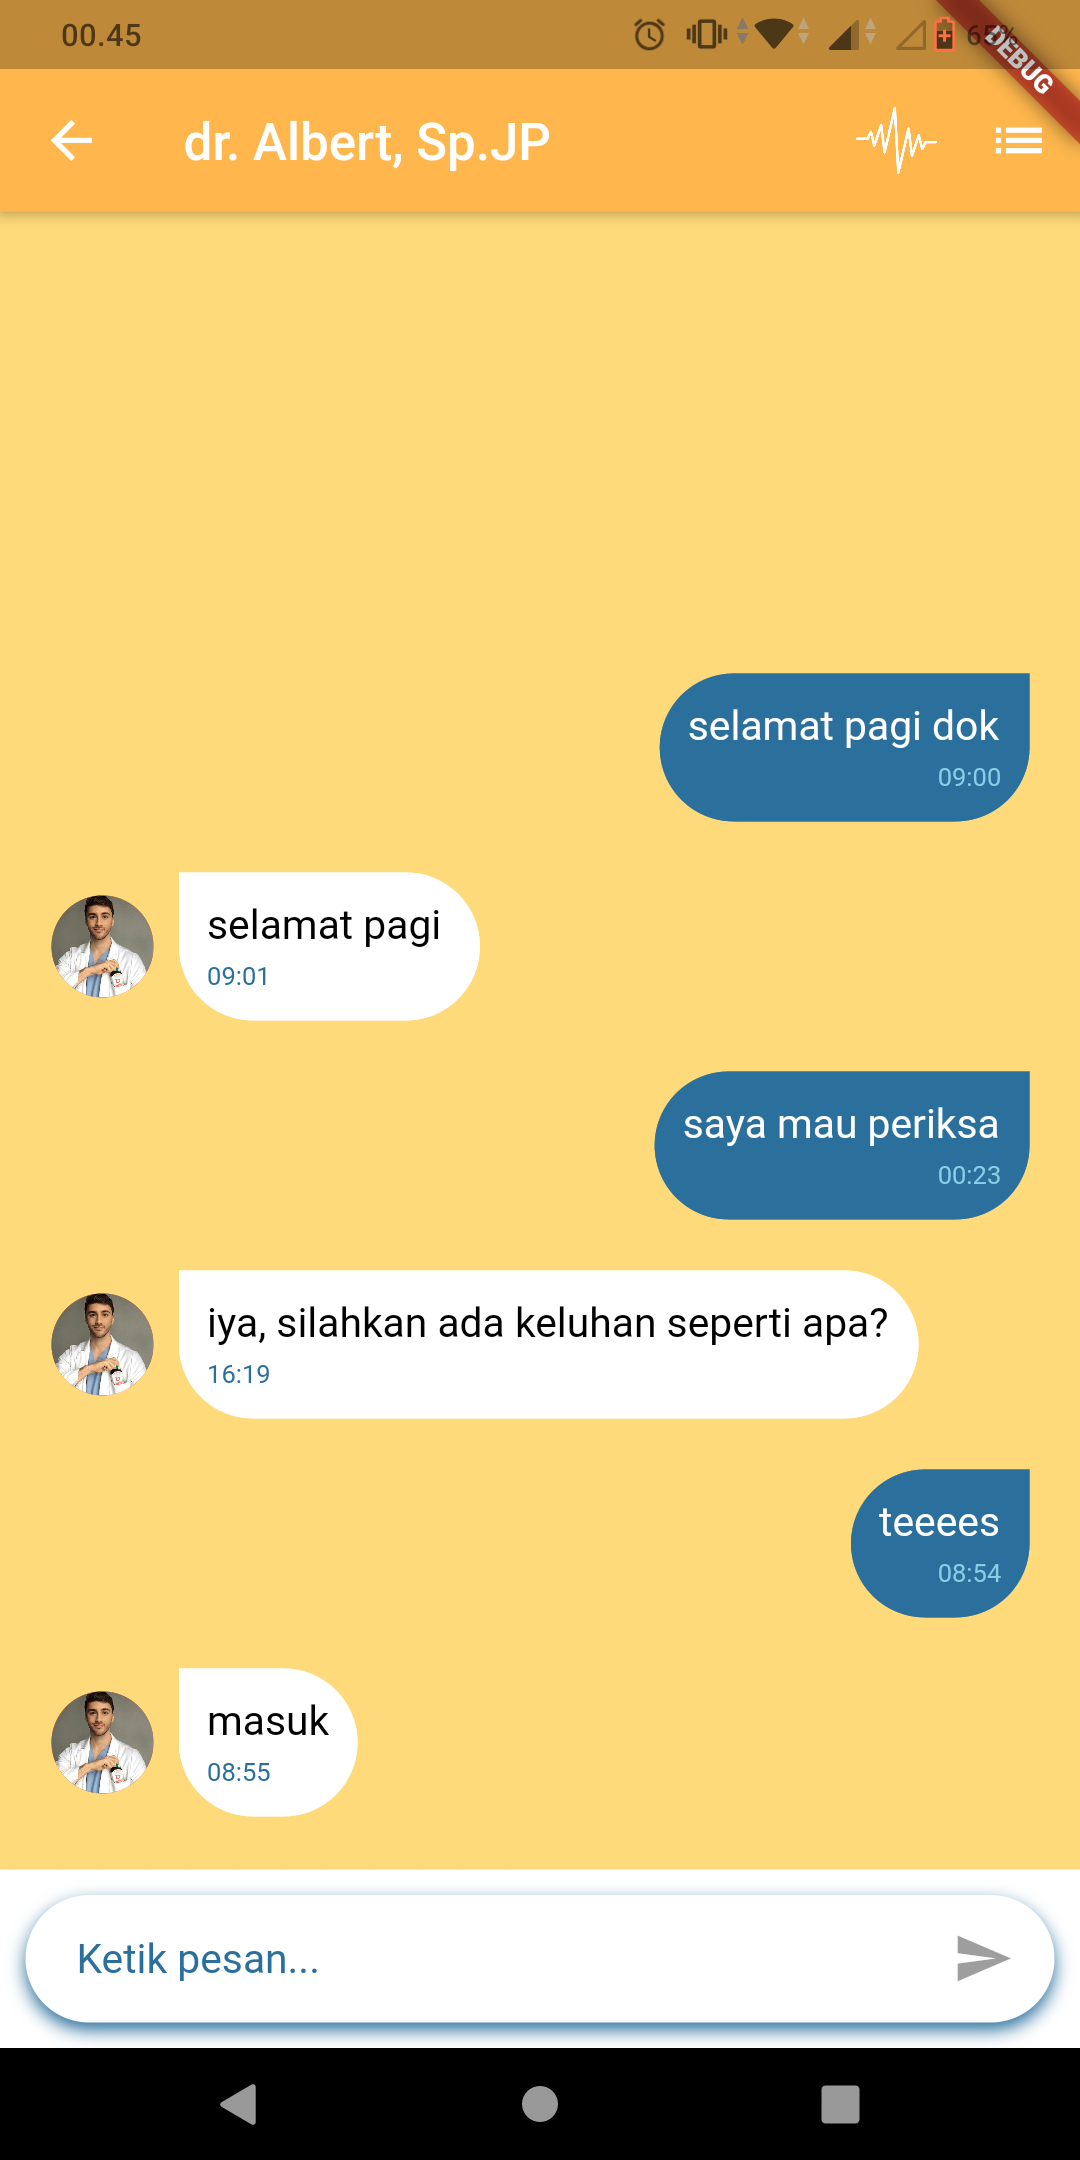
\includegraphics[width=0.4\textwidth]{img/layar_chatpasien.png}
	\caption{Implementasi UI Chatscreen Pasien.}
	\label{fig:3.10}
\end{figure}

Sedangkan untuk tampilan screen chat dokter dapat dilihat pada Gambar \ref{fig:3.11}.

\begin{figure}[H] \centering
	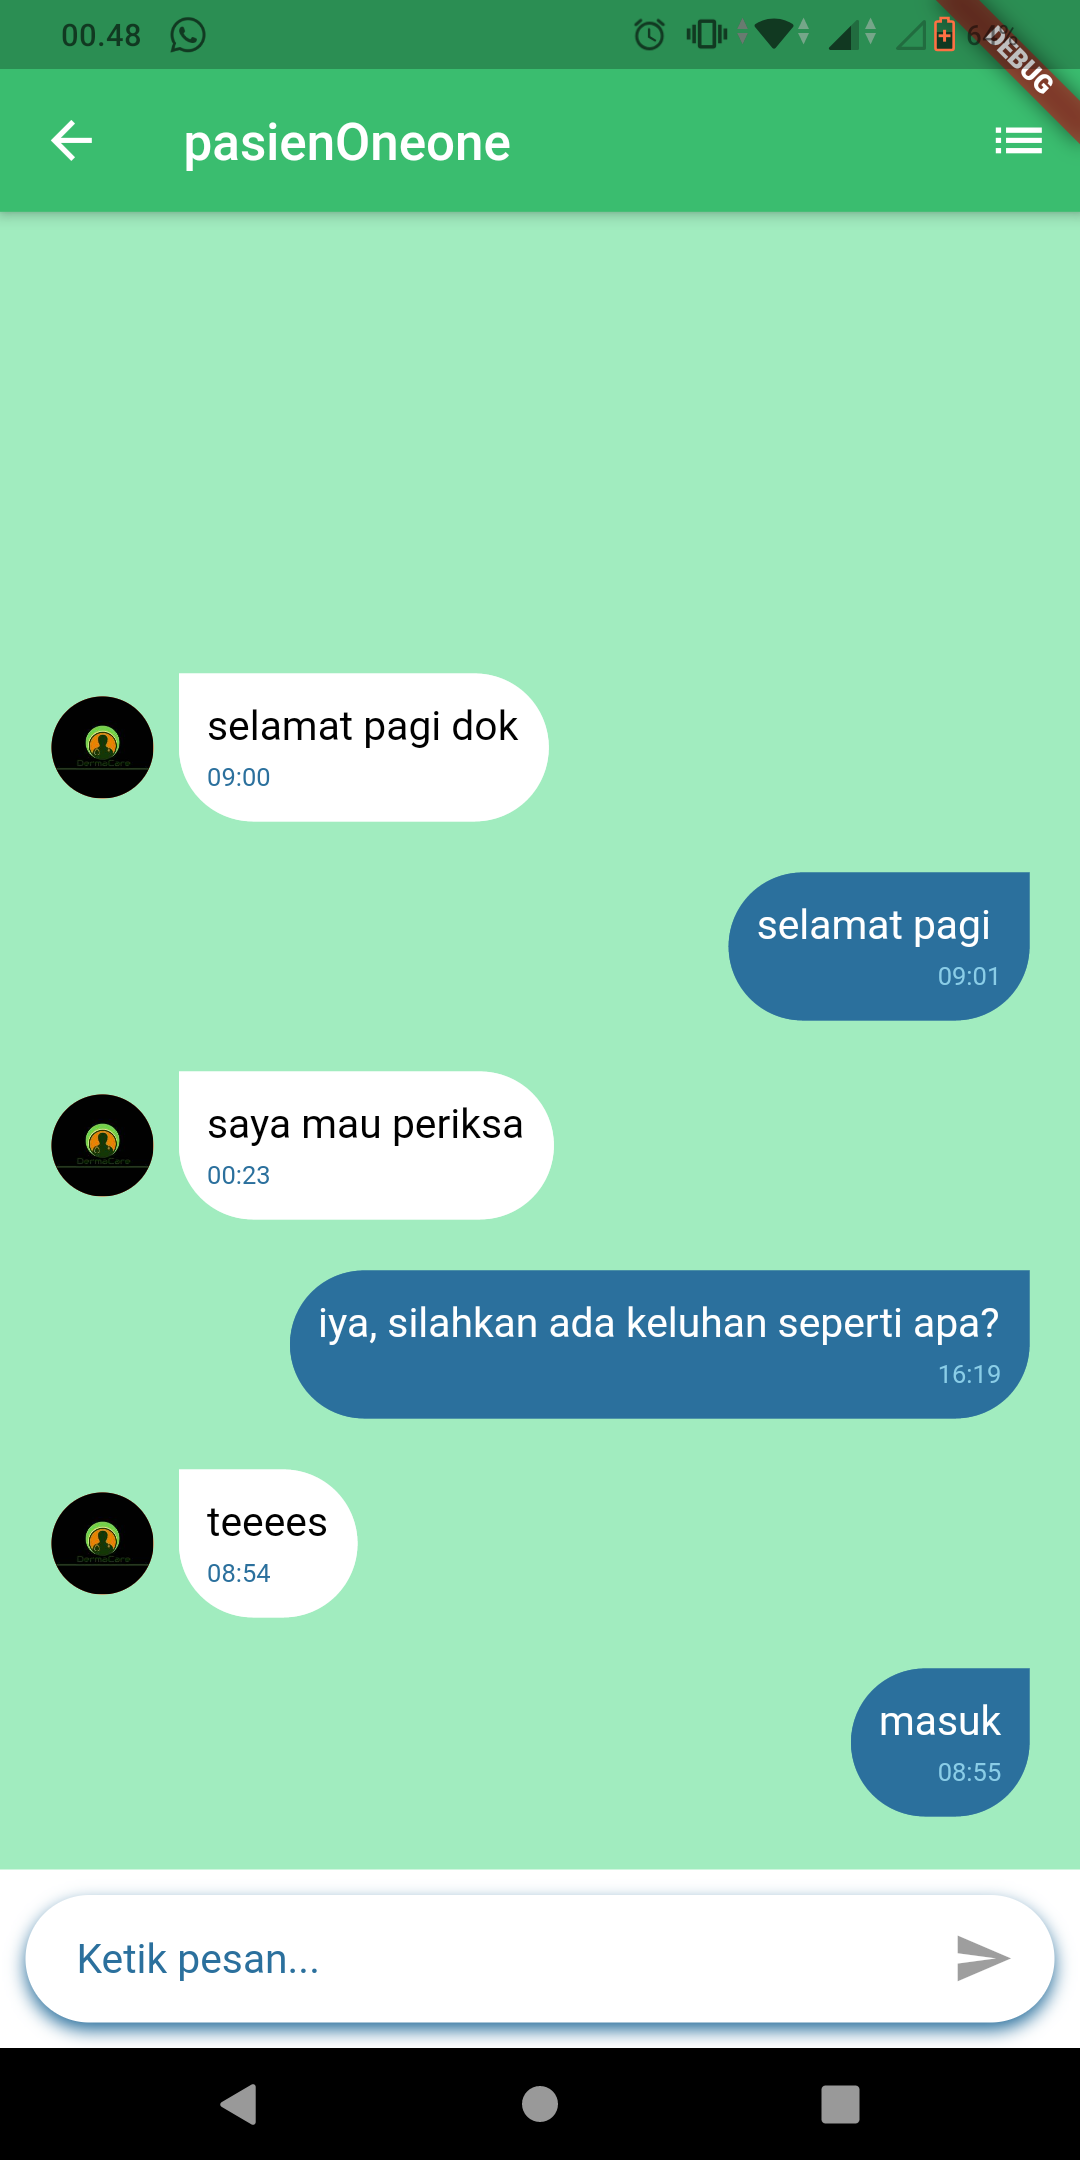
\includegraphics[width=0.4\textwidth]{img/layar_chatdokter.png}
	\caption{Implementasi UI Chatscreen Dokter.}
	\label{fig:3.11}
\end{figure}

Pada layar chat juga terdapat icon di pojok kanan atas yang berfungsi untuk jalan pintas. Pada Chatscreen pasien terdapat 2 icon yaitu icon sinyal ECG dan icon tiga garis. Icon sinyal ECG akan mengarahkan pasien menuju layar rekam data ECG sedangkan icon tiga garis akan mengarahkan pasien menuju layar riwayat rekaman ECG.
Sedangkan pada Chatscreen dokter hanya terdapat satu icon yang akan mengarahkan dokter menuju layar riwayat rekaman ECG yang dikirimkan oleh pasien. 
\clearpage


\cleardoublepage
\chapter{HASIL DAN PENGUJIAN}
\vspace{1ex}

\section*{}
Pada bab ini dipaparkan hasil pengujian serta analisa dari de-
sain sistem dan implementasi .Pengujian dilakukan guna mengetahui tingkat kesalahan dan menarik kesimpulan dari sistem yang telah dibuat.

Pada pengujian ini digunakan \textit{Smartphone Android} dengan spesifikasi hardware seperti pada tabel \ref{tabel:4.0}.
\begin{table}[h!]
		\caption{Spesifikasi \textit{Smartphone} yang Digunakan}
	\begin{tabular}{|l|l|}
		\hline
		\textbf{CPU} & \begin{tabular}[c]{@{}l@{}}Octa-core (4x1.8 GHz Kryo 260 Gold \\ \& 4x1.6 GHz Kryo 260 Silver)\end{tabular} \\ \hline
		\textbf{Internal}       & \begin{tabular}[c]{@{}l@{}}32GB 3GB RAM\end{tabular}  \\ \hline
		\textbf{Chipset}          & Qualcomm SDM636 Snapdragon 636 (14 nm)             \\ \hline
		\textbf{OS}     & Android 8.1 (Oreo), upgradable to Android 9.0 (Pie) \\ \hline
		\textbf{GPU} & Adreno 509         \\ \hline
		\textbf{Bluetooth} & 5.0, A2DP, LE         \\ \hline
	\end{tabular}
	\vspace{1ex}
	\caption{Spesifikasi \textit{Smartphone} yang Digunakan}
	\label{tabel:4.0}
\end{table}




\section{Pengujian Rekaman Data Selama 15 Menit}
\vspace{1ex}
Pengujian ini dilakukan untuk menentukan baudrate bluetooth HC-05 yang akan digunakan dan delay yang diprogram pada arduino. Pada pengujian ini dilakukan dengan cara melakukan rekaman data dengan target durasi rekaman adalah 15 menit. Untuk menentukan delay dan baudrate yang akan digunakan maka pada pengujian ini dilakukan percobaan dengan delay dan baudrate yang berbeda-beda. Untuk delay sendiri memiliki 3 percobaan yaitu delay 1 ms, delay 5 ms, dan delay 10 ms. Sedangkan baudrate yang digunakan untuk percobaan terdapat 3 tahap yaitu 9600, 38400, dan 57600. Berikut ini merupakan tabel hasil pengujian rekaman data selama 15 (Tabel \ref{tabel:4.0.0})
\begin{table}[H]
	\caption{Tabel hasil percobaan rekaman data dengan target 15 menit}
	\begin{tabular}{|c|c|c|c|c|}
		\hline
		\multicolumn{1}{|c|}{{\color[HTML]{000000} \textbf{Delay}}} & \multicolumn{1}{|c|}{\textbf{Baudrate}} &
		\multicolumn{1}{|c|}{ \textbf{\textit{Force}}} &
		\multicolumn{1}{|c|}{\textbf{Durasi}} &
		\multicolumn{1}{|c|}{\textbf{Sampling}}  \\
		(ms) &  \textbf{HC-05}  & \textbf{\textit{close}}  & \textbf{dicapai} & \textbf{rate}  \\
		&  &  &   & (sampel/detik)  \\ \hline
		
		10 & 9600 & tidak & 15 menit & 50  \\ \hline
		5 & 9600 & ya & 2 menit & 68  \\
		& & & 58.20 detik & \\ \hline
		1 & 9600 & ya & 4 menit & 90  \\ & & & 22.98 detik & \\\hline
		10 & 38400 & ya & 3 menit & 72  \\ & & & 23.65 detik & \\\hline
		5 & 38400 & ya & 1 menit & 114  \\ & & & 52.64 detik & \\ \hline
		1 & 38400 & ya & 2 menit & 216  \\ & & & 14.68 detik & \\ \hline
		10 & 57600 & ya & 2 menit & 112  \\ & & & 05.98 detik & \\ \hline
		5 & 57600 & ya & 2 menit & 125  \\ & & & 51.81 detik & \\ \hline
		1 & 57600 & ya & 2 menit & 270  \\ & & & 23.52 detik & \\ \hline
		%10 & 115200 & ya & 3 menit & 117  \\ & & & 52.15 detik & \\ \hline
		%5 & 115200 & ya & 1 menit & 139  \\ & & & 42.05 detik & \\ \hline
		%1 & 115200 & ya & 1 menit & 327  \\ & & & 36.90 detik & \\ \hline
		
	\end{tabular}
	\vspace{1ex}
	
	\label{tabel:4.0.0}
\end{table}

Dapat dilihat pada tabel diatas memiliki 5 kolom yaitu Delay, Baudrate HC-05, Force close, Durasi dicapai, dan \textit{sampling rate}. Delay merupakan durasi jeda waktu yang digunakan pada loop arduino. Baudrate HC-05 merupakan kecepatan pengiriman data oleh modul bluetooth HC-05. Force close merupakan kejadian dimana aplikasi menutup dengan sendirinya. Durasi dicapai merupakan lama waktu rekaman yang telah didapat sampai dengan aplikasi force close. \textit{sampling rate} merupakan jumlah data atau sampel yang didapat selama satu detik.

Pada percobaan pertama dilakukan dengan menggunakan delay 10 ms, baudrate HC-05 sebesar 9600, dan frekuensing sampling sebesar 50 data/detik. Pada percobaan pertama berjalan lancar hingga aplikasi dapat merekam data selama 15 menit. Percobaan kedua dilakukan dengan mengubah delay arduino menjadi 5 ms, \textit{sampling rate} yang didapat adalah 68 data/detik, pada percobaan ini aplikasi tertutup dengan sendirinya (\textit{force close}) setelah merekam selama 2 menit 58.20 detik. Percobaan ketiga dilakukan menggunakan delay 1 ms, dengan baudrate tetap sebesar 9600, \textit{sampling rate} yang diperoleh sebesar 90 data/detik, pada percobaan ketiga aplikasi mengalami \textit{force close} setelah merekam selama 4 menit 22.98 detik. Percobaan keempat menggunakan delay 10 ms, dengan baudrate HC-05 diperbesar menjadi 38400, \textit{sampling rate} pada percobaan ini sebesar 72 data/detik, pada percobaan keempat ini aplikasi juga mengalami \textit{force close} setelah merekam selama 3 menit 23.65 detik. Percobaan kelima menggunakan delay sebesar 5 ms, dengan baudrate 38400, \textit{sampling rate} yang diperoleh
sebesar 114 data/detik, dan seperti sebelumnya aplikasi mengalami \textit{force close} setelah merekam selama 1 menit 52.64 detik. Percobaan keenam dilakukan menggunakan delay sebesar 1 ms, dengan baudrate yang sama yaitu 38400, \textit{sampling rate} yang diperoleh sebesar 216 data/detik, aplikasi mengalami \textit{force close} setelah merekam selama 2 menit 14.68 detik. Pada percobaan ketujuh aplikasi juga mengalami \textit{force close}, durasi yang dicapai selama 2 menit 05.98 detik, percobaan ini menggunakan delay arduino sebesar 10 ms, dengan baudrate yang diperbesar menjadi 57600, dan \textit{sampling rate} yang diperoleh sebesar 112 data/detik. Percobaan kedelapan dilakukan menggunakan delay arduino sebesar 5 ms, dengan baudrate sebesar 57600, diperoleh \textit{sampling rate} sebesar 125 data/detik, aplikasi mengalami \textit{force close} setelah merekam selama 2 menit 51.81 detik. Percobaan kesembilan dilakukan dengan menggunakan delay arduino sebesar 1 ms, dengan baudrate sebesar 57600, diperoleh \textit{sampling rate} sebesar 270, aplikasi mengalami \textit{force close} setelah merekam selama 2 menit 23.52 detik. 

Berdasarkan tabel \ref{tabel:4.0.0} dapat dilihat pada kolom \textit{force close} dimana hampir pada semua percobaan yang telah dilakukan mengalami force close pada aplikasi. Apabila dilihat pada kolom durasi dicapai, durasi waktu yang didapat saat aplikasi force close tidak pasti, tetapi sebagian besar aplikasi mengalami force close pada menit ke-2. Sedangkan apabila kolom Force close dihubungkan kolom \textit{sampling rate}
maka aplikasi hanya dapat berjalan dengan baik hingga menit ke-15 dengan menggunakan fruekuensi sampling 50 sampel/detik, untuk frekuensi selain 50 sampel/detik tersebut aplikasi mengalami force close. Berdasarkan analisa maka dapat  semakin besar \textit{sampling rate} yang digunakan maka semakin besar kemungkinan force close pada aplikasi.

Apabila dilihat pada tabel \ref{tabel:4.0} versi \textit{bluetooth} pada \textit{smartphone} adalah versi 5.0. Kecepatan transfer \textit{bluetooth} 5.0 adalah 3 Mbps sedangkan kecepatan bluetooth HC-05 adalah 1 Mbps dan bisa dicustom sampai 1.3 Mbps. \textit{force close} minimal pada \textit{sampling rate} sebesar 68 sampel tiap detik.
Sedangkan sampel tersebut merupakan string yang terdiri dari antara 7 sampai 9 karakter. Apabila dihitung 10 karakter tiap sampel maka aplikasi mengalami \textit{force close} saat menerima data 680 byte tiap detik sehingga masalah \textit{force close} tidak terdapat pada versi bluetooth smartphone yang memiliki kecepatan 3 Mbps dan HC-05 yang berkecepatan 1 Mbps. Setelah dilakukan kaji ulang pada aplikasi kemudian ditemukan masalah penyebab \textit{force close}. \textit{Force close}
terjadi dikarenakan adanya \textit{pop up} pada aplikasi pada saat menerima data, sedangkan \textit{pop up} sendiri memiliki animasi yang berdurasi kurang lebih 1 detik, dilain sisi \textit{pop up} tersebut dipaksa muncul 68 kali dalam 1 detik, sehingga terdapat \textit{pop up} yang bertumpuk pada aplikasi dan menyebabkan \textit{force close}.

Setelah aplikasi tidak mengalami force, dilakukan percobaan
dengan baudrate 57600. Aplikasi dapat melakukan rekaman data
maksimal dengan \textit{sampling rate} sebesar 280 data tiap detik tanpa
mengalami force close. Aplikasi dapat berjalan lebih lancar tanpa
maengalami macet apabila \textit{sampling rate} lebih sedikit. Data percobaan yang baru telah didapatkan seperti pada tabel \ref{tabel:4.0.1}.


\begin{table}[H]
	\caption{Tabel hasil percobaan rekaman data selama 15 menit}
	\begin{tabular}{|c|c|c|c|c|c|}
		\hline
		\multicolumn{1}{|c|}{{\color[HTML]{000000} \textbf{Delay}}} & \multicolumn{1}{|c|}{\textbf{Uji}} &
		\multicolumn{1}{|c|}{ \textbf{Durasi}} &
		\multicolumn{1}{|c|}{\textbf{Jumlah}} &
		\multicolumn{1}{|c|}{\textbf{\textit{Sampling}}}  & 
		\multicolumn{1}{|c|}{\textbf{\textit{Force}}} \\
		(ms) &  \textbf{ke-}  & \textbf{rekaman}  & \textbf{data} & \textbf{\textit{rate}}  & \textit{\textbf{close}}\\
		&  &  &  \textbf{diterima} & &  \\ \hline
		
		\multirow{5}{*}{5} &1& 15:00.09 &118317 &131 & tidak \\
		\cline{2-6}&2 &15.00.55 & 118214 &131 & tidak\\ 
		\cline{2-6}&3 &15.00.73 & 118235 &131 & tidak\\ 
		\cline{2-6}&4 &15.01.75 & 118229 &131 & tidak\\ 
		\cline{2-6}&5 &15.00.34 & 118143 &131 & tidak\\ 
		\hline
		\multirow{5}{*}{4} &1& 15:00.76 &136919 &152 & tidak \\
		\cline{2-6}&2 &15.00.53 & 136070 &151 & tidak\\ 
		\cline{2-6}&3 &15.01.48 & 136145 &151 & tidak\\ 
		\cline{2-6}&4 &15.02.32 & 136544 &151 & tidak\\ 
		\cline{2-6}&5 &15.00.46 & 136297 &151 & tidak\\ 
		\hline
		\multirow{5}{*}{3} &1& 15:00.49 &161161 &179 & tidak \\
		\cline{2-6}&2 &15.14.86 & 162735 &180 & tidak\\ 
		\cline{2-6}&3 &15.00.65 & 160370 &178 & tidak\\ 
		\cline{2-6}&4 &15.00.54 & 161134 &179 & tidak\\ 
		\cline{2-6}&5 &15.00.76 & 161743 &179 & tidak\\ 
		\hline
		\multirow{5}{*}{2} &1& 15:00.61 &196266 &218 & tidak \\
		\cline{2-6}&2 &15.00.42 & 194900 &216 & tidak\\ 
		\cline{2-6}&3 &15.00.41 & 194790 &216 & tidak\\ 
		\cline{2-6}&4 &15.00.44 & 194999 &216 & tidak\\ 
		\cline{2-6}&5 &15.00.61 & 195129 &216 & tidak\\ 
		\hline
		\multirow{5}{*}{1} &1& 15:00.13 &248298 &275 & tidak \\
		\cline{2-6}&2 &15.00.34 & 248573 &276 & tidak\\ 
		\cline{2-6}&3 &15.00.41 & 248790 &276 & tidak\\ 
		\cline{2-6}&4 &15.00.54 & 252201 &280 & tidak\\ 
		\cline{2-6}&5 &15.00.56 & 249855 &277 & tidak\\ 
		\hline
	\end{tabular}
	\vspace{1ex}
	
	\label{tabel:4.0.1}
\end{table}


\section{Pengujian Waktu Pengiriman Data Menuju Database}
\vspace{1ex}
Pengujian ini dilakukan untuk mengetahui seberapa lama waktu yang dibutuhkan untuk mengupload data menuju database. Pengujian dilakukan dengan cara merekam data ECG secara bertahap untuk diupload yaitu dari 1 menit sampai 15 menit. Pada pengujian ini baudrate modul HC-05 yang digunakan adalah 9600 dan delay yang digunakan pada arduino sebesar 10 ms serta data diupload menuju server online. Dari masing-masing tahap rekaman tersebut akan dibandingkan berapa waktu yang dibutuhkan untuk upload data. Berikut merupakan tabel hasil pengujian durasi upload data (Tabel \ref{tabel:4.2}).
\begin{table}[H]
	\caption{Tabel hasil percobaan durasi upload}
	\begin{tabular}{|c|c|c|c|c|c|}
		\hline
		\multicolumn{1}{|c|}{{\color[HTML]{000000} \textbf{Delay}}} & \multicolumn{1}{|c|}{\textbf{Uji}} &
		\multicolumn{1}{|c|}{ \textbf{Durasi}} &
		\multicolumn{1}{|c|}{\textbf{Jumlah}} &
		\multicolumn{1}{|c|}{\textbf{\textit{Sampling}}}  & 
		\multicolumn{1}{|c|}{\textbf{\textit{Force}}} \\
		(ms) &  \textbf{ke-}  & \textbf{rekaman}  & \textbf{data} & \textbf{\textit{rate}}  & \textit{\textbf{close}}\\
		&  &  &  \textbf{diterima} & &  \\ \hline
		
		\multirow{5}{*}{5} &1& 15:00.09 &118317 &131 & 02:25 \\
		\cline{2-6}&2 &15.00.55 & 118214 &131 & 02:27\\ 
		\cline{2-6}&3 &15.00.73 & 118235 &131 & 02:46\\ 
		\cline{2-6}&4 &15.01.75 & 118229 &131 & 02:58\\ 
		\cline{2-6}&5 &15.00.34 & 118143 &131 & 02:44\\ 
		\hline
		\multirow{5}{*}{4} &1& 15:00.76 &136919 &152 & 01:40 \\
		\cline{2-6}&2 &15.00.53 & 136070 &151 & 01:38\\ 
		\cline{2-6}&3 &15.01.48 & 136145 &151 & 01:19\\ 
		\cline{2-6}&4 &15.02.32 & 136544 &151 & 00:55\\ 
		\cline{2-6}&5 &15.00.46 & 136297 &151 & 00:47\\ 
		\hline
		\multirow{5}{*}{3} &1& 15:00.49 &161161 &179 & 03:37 \\
		\cline{2-6}&2 &15.14.86 & 162735 &180 & 01:37\\ 
		\cline{2-6}&3 &15.00.65 & 160370 &178 & 02:36\\ 
		\cline{2-6}&4 &15.00.54 & 161134 &179 & 03:15\\ 
		\cline{2-6}&5 &15.00.76 & 161743 &179 & 01:45\\ 
		\hline
		\multirow{5}{*}{2} &1& 15:00.61 &196266 &218 & 01:50 \\
		\cline{2-6}&2 &15.00.42 & 194900 &216 & 03:34\\ 
		\cline{2-6}&3 &15.00.41 & 194790 &216 & 02:15\\ 
		\cline{2-6}&4 &15.00.44 & 194999 &216 & 01:43\\ 
		\cline{2-6}&5 &15.00.61 & 195129 &216 & 03:22\\ 
		\hline
		\multirow{5}{*}{1} &1& 15:00.13 &248298 &275 & 04:51 \\
		\cline{2-6}&2 &15.00.34 & 248573 &276 & 05:05\\ 
		\cline{2-6}&3 &15.00.41 & 248790 &276 & 02:24\\ 
		\cline{2-6}&4 &15.00.54 & 252201 &280 & 04:56\\ 
		\cline{2-6}&5 &15.00.56 & 249855 &277 & 02:04\\ 
		\hline
	\end{tabular}
	\vspace{1ex}
	
	\label{tabel:4.2}
\end{table}

Dapat dilihat dari tabel \ref{tabel:4.2} memiliki 6 kolom yaitu Delay,
Uji ke-, Durasi rekaman, Jumlah Data diterima,\textit{ Sampling rate} dan
Durasi upload. Delay merupakan jeda waktu yang digunakan pada
loop arduino. Kolom Uji ke- merupakan nomor urutan percobaan
yang telah dilakukan. Durasi rekaman merupakan jangka waktu
yang dilakukan saat merekam data. Jumlah Data diterima merupakan jumlah data yang dapat disampaikan oleh modul bluetooth
HC-05 dari Arduino. \textit{Sampling rate} merupakan jumlah sampel yang
didapatkan dalam setiap detik. Dan yang terakhir adalah Durasi
upload yang mana merupakan jangka waktu yang diperlukan untuk
mengupload data dari aplikasi menuju database.


Berdasarkan tabel \ref{tabel:4.2} dapat dilihat perbandingan durasi upload antara \textit{sampling rate} 131 hingga \textit{sampling rate} 280. Dari tabel
tersebut dapat dilihat durasi upload yang diperlukan tidak pasti
atau juga dapat dikatakan tidak linier apabila dibandingkan dengan durasi rekaman. Hal tersebut karena database ada pada server
online maka tergantung jaringan internet yang digunakan. Apabila
pada saat upload data memiliki jaringan internet yang bagus maka
durasi upload akan berjalan lebih cepat. Sebaliknya apablika pada saat upload data memiliki jaringan internet yang kurang bagus
maka proses upload akan berjalan lebih lama. Pada tabel 4.5 data
durasi waktu upload terlama diperoleh pada delay waktu 1 ms pada
percobaab ke-2 yaitu 5 menit lebih 5 detik.

\section{Pengujian kesesuaian data dari arduino dan data di aplikasi}
\vspace{1ex}
Pengujian ini dilakukan untuk melihat perbedaan data yang dikirim dari arduino dengan data yang telah diproses oleh aplikasi. Pengujian ini dilakukan dengan cara melakukan rekaman data selama 1 menit. Percobaan dilakukan sebanyak 5 kali percobaan, data percobaan kemudian dibandingkan 

Data pada arduino ditampilkan menggunakan serial monitor dan untuk aplikasi ditampilkan pada box putih bagian bawah. Dapat dilihat pada gambar \ref{fig:4.2}. Pada gambar tersebut dapat dilihat serial monitor telah menampilkan data yang dikirim oleh arduino terdapat 3 bagian data yaitu \textbf{sampel:data ECG$\mid$detik$\mid$} tetapi data yang dikirim hanya data \textbf{ECG$\mid$detik$\mid$} sedangkan untuk urutan sampel akan diproses pada aplikasi. Hal tersebut dikarenakan sampel pertama yang dikirim dari arduino belum tentu sampai pada aplkasi, maka aplikasi perlu menentukan sampel yang pertama. 
\begin{figure}[H] \centering
	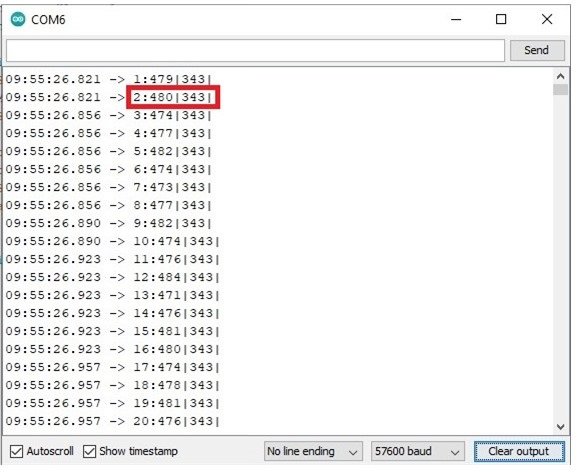
\includegraphics[width=0.7\textwidth]{img/percob/Slide1}

	(a)
	
	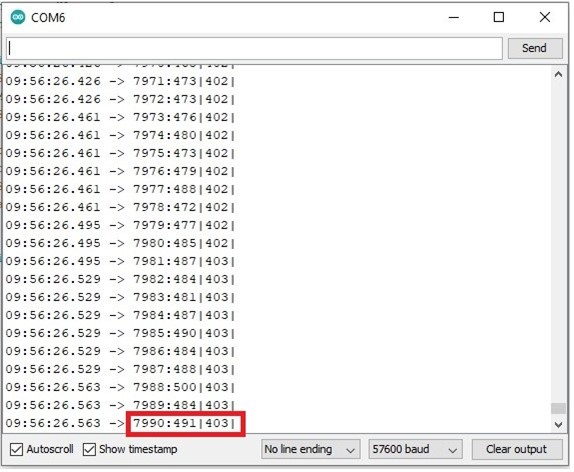
\includegraphics[width=0.7\textwidth]{img/percob/Slide2}
	
	(b)
	
	\caption{Percobaan 1 : (a)Data awal yang dikirim dari arduino, (b)Data akhir yang dikirim arduino.}
	\label{fig:4.2}
\end{figure}
\vspace{1ex}
Dapat dilihat pada Gambar \ref{fig:4.2}, tanda "$\mid$" yang ada pada data tersebut diperlukan untuk melakukan split pada program aplikasi untuk memisahkan data ECG dengan detik. Pada tanda kotak berwarna merah berisi "2:480$\mid$343$\mid$" yang mana angka "2" adalah urutan sampel dari arduino, kemudian angka "480" adalah data sensor, dan "343" merupakan detik. Pada percobaan pertama, data awal yang terkirim oleh arduino adalah 480 pada sampel ke-2 dan data terakhir yang terkirim adalah 491 pada sampel ke-7990. Apabila dihitung maka jumlah sampel yang terkirim adalah 7989 sampel dalam satu menit.
\begin{figure}[H] \centering
	\begin{subfigure}{0.45\textwidth}
		\centering
		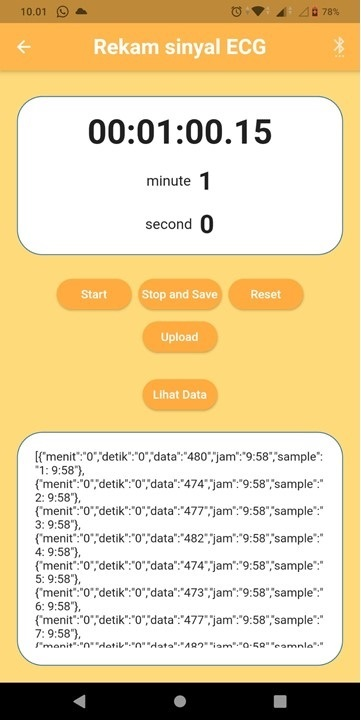
\includegraphics[width=1\linewidth]{img/percob/Slide11a}	  
		\caption{}		
	\end{subfigure}
	\begin{subfigure}{0.45\textwidth}
		\centering
		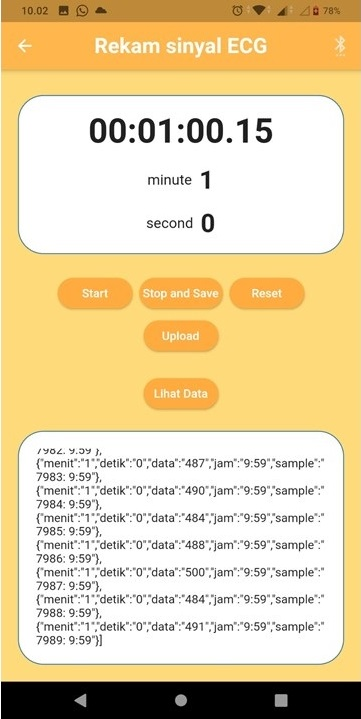
\includegraphics[width=1\linewidth]{img/percob/Slide11b.jpg}	  
		\caption{}		
	\end{subfigure}
	\caption{Percobaan 1: (a) Data awal yang diterima aplikasi, (b) Data akhir yang diterima aplikasi.}
	\label{fig:4.2.0}
\end{figure}
\vspace{1ex}
Gambar \ref{fig:4.2.0} merupakan tampilan data yang diterima aplikasi. Dapat dilihat pada gambar tersebut, data yang ada aplikasi adalah menit, detik, data, jam, dan sampel. Menit tersebut didapatkan dari memproses detik yang telah dikirim dari arduino. Detik didapatkan dari data yang dikirim oleh arduino. Data merupakan data ECG yang dikirim oleh arduino. Jam merupakan data penjumlahan antara waktu mulai rekaman dengan detik yang diperoleh dari arduino. Sampel didapat dari proses penomoran data pada aplikasi.  Layar sebelah kiri menunjukkan data pertama yang diterima adalah 480 dan layar sebelah kanan menunjukkan data terakhir yang diterima aplikasi adalah 491. Jumlah data yang diterima oleh aplikasi dapat dilihat pada nomor "sample" yaitu 7989 sampel. Berikutnya adalah gambar percobaan kedua. 
\begin{figure}[H] \centering
	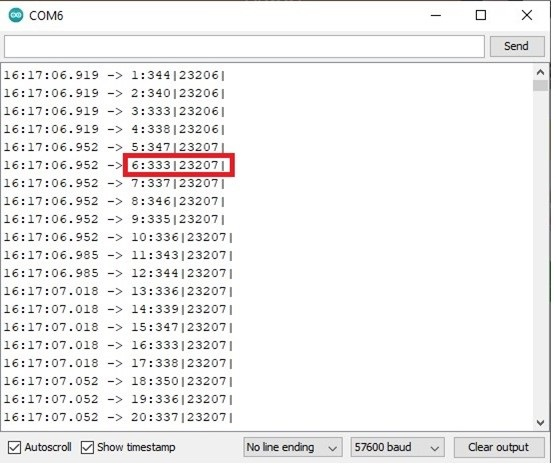
\includegraphics[width=0.7\textwidth]{img/percob/Slide3}
	
	(a)
	
	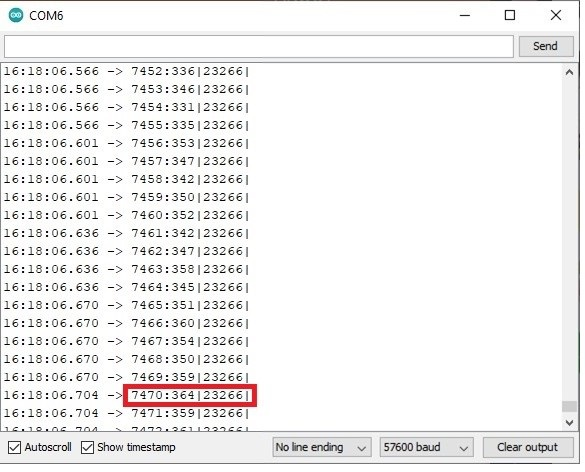
\includegraphics[width=0.7\textwidth]{img/percob/Slide4}
	
	(b)
	
	\caption{Percobaan 2 : (a)Data awal yang dikirim dari arduino, (b)Data akhir yang dikirim arduino.}
	\label{fig:4.2.1}
\end{figure}
\vspace{1ex}
Dapat dilihat pada Gambar \ref{fig:4.2.1}, pada bagian (a) data awal yang terkirim oleh arduino adalah 333 yang merupakan sampel keenam dan pada bagian (b) data terakhir yang terkirim adalah 364 yang merupakan sampel ke-7470. Jumlah data yang dikirim oleh arduino adalah 7465 sampel.

\begin{figure}[H] \centering
	\begin{subfigure}{0.45\textwidth}
		\centering
		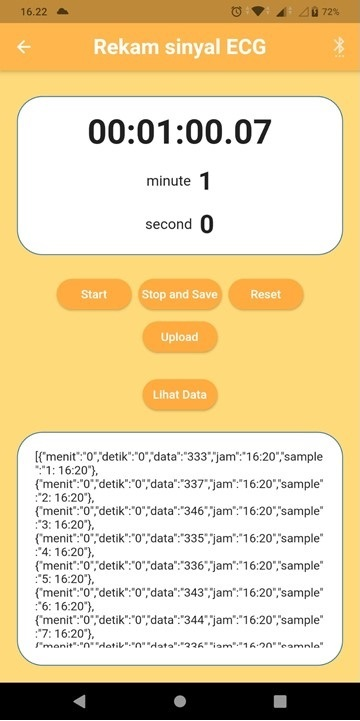
\includegraphics[width=1\linewidth]{img/percob/Slide12a}	  
		\caption{}		
	\end{subfigure}
	\begin{subfigure}{0.45\textwidth}
		\centering
		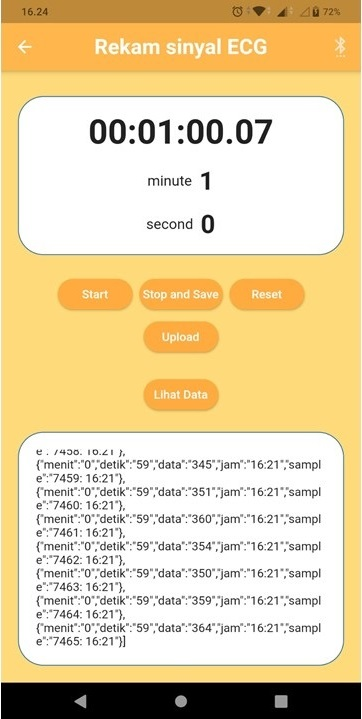
\includegraphics[width=1\linewidth]{img/percob/Slide12b.jpg}	  
		\caption{}		
	\end{subfigure}	
	\caption{Percobaan 2: (a) Data awal yang diterima aplikasi, (b) Data akhir yang diterima aplikasi.}
	\label{fig:4.2.2}
\end{figure}
\vspace{1ex}
Gambar \ref{fig:4.2.2} merupakan tampilan data yang diterima aplikasi pada percobaan kedua. Layar sebelah kiri menunjukkan data pertama yang diterima adalah 333 dan layar sebelah kanan menunjukkan data terakhir yang diterima aplikasi adalah 364. Jumlah data yang diterima oleh aplikasi dapat dilihat pada nomor "sample" yaitu 7465 sampel. Berikutnya adalah gambar percobaan ketiga. 

\begin{figure}[H] \centering
	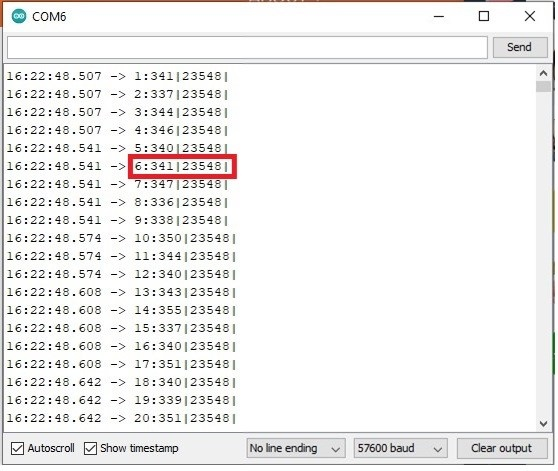
\includegraphics[width=0.7\textwidth]{img/percob/Slide5}
	
	(a)
	
	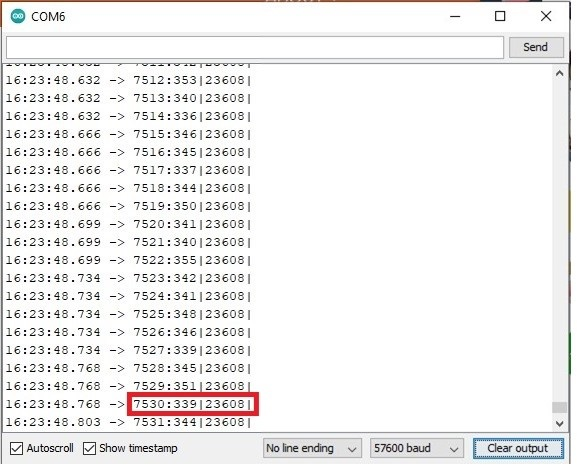
\includegraphics[width=0.7\textwidth]{img/percob/Slide6}
		
	(b)
	
	\caption{Percobaan 3 : (a)Data awal yang dikirim dari arduino, (b)Data akhir yang dikirim arduino.}
	\label{fig:4.2.3}
\end{figure}
\vspace{1ex}
Dapat dilihat pada Gambar \ref{fig:4.2.3}, pada bagian (a) data awal yang terkirim oleh arduino adalah 341 yang merupakan sampel keenam dan pada bagian (b) data terakhir yang terkirim adalah 339 yang merupakan sampel ke-7470. Jumlah data yang dikirim oleh arduino adalah 7525 sampel.

\begin{figure}[!h] \centering
	\begin{subfigure}{0.45\textwidth}
		\centering
		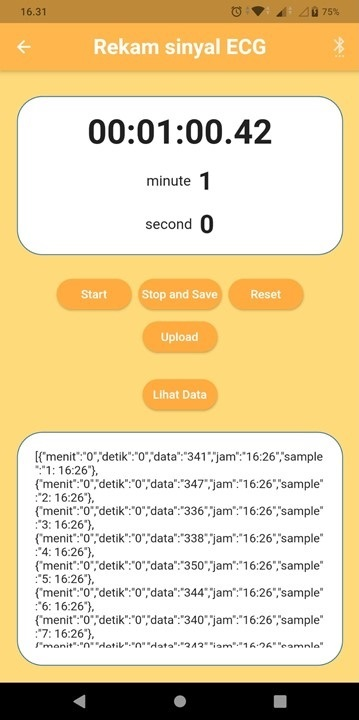
\includegraphics[width=1\linewidth]{img/percob/Slide13a}	  
		\caption{}		
	\end{subfigure}
	\begin{subfigure}{0.45\textwidth}
		\centering
		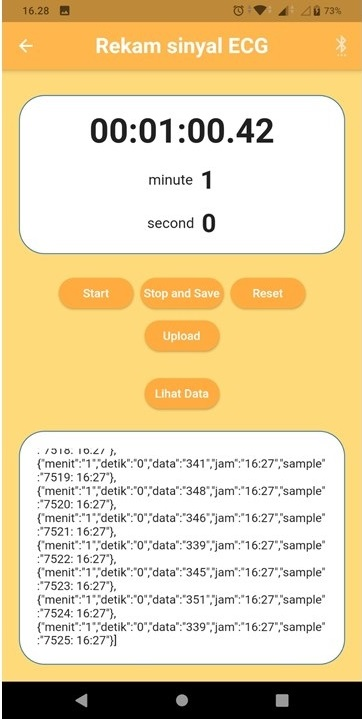
\includegraphics[width=1\linewidth]{img/percob/Slide13b.jpg}	  
		\caption{}		
	\end{subfigure}
	
	\caption{Percobaan 3: (a) Data awal yang diterima aplikasi, (b) Data akhir yang diterima aplikasi.}
	\label{fig:4.2.4}
\end{figure}
Gambar \ref{fig:4.2.4} merupakan tampilan data yang diterima aplikasi. Layar sebelah kiri menunjukkan data pertama yang diterima adalah 341 dan layar sebelah kanan menunjukkan data terakhir yang diterima aplikasi adalah 339. Jumlah data yang diterima oleh aplikasi dapat dilihat pada nomor "sample" yaitu 7525 sampel. Berikutnya adalah gambar percobaan keempat. 
\begin{figure}[H] \centering
	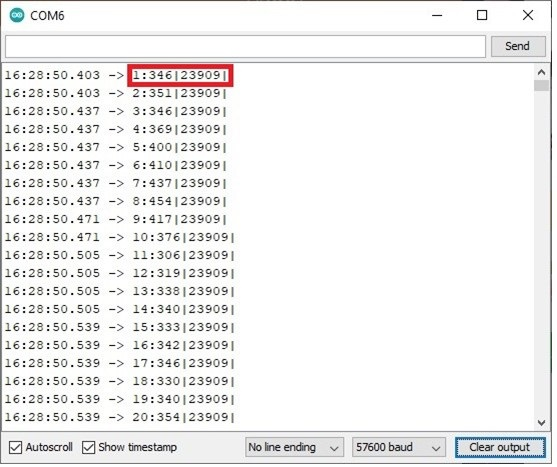
\includegraphics[width=0.7\textwidth]{img/percob/Slide7}
	
	(a)
	
	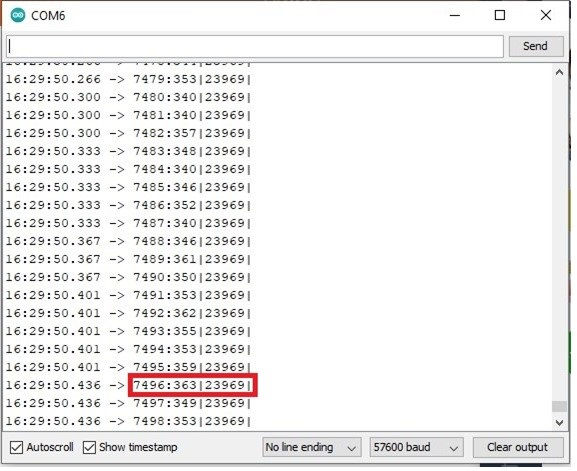
\includegraphics[width=0.7\textwidth]{img/percob/Slide8}
	
	(b)
	
	\caption{Percobaan 4 : (a)Data awal yang dikirim dari arduino, (b)Data akhir yang dikirim arduino.}
	\label{fig:4.2.5}
\end{figure}
\vspace{1ex}
Pada gambar \ref{fig:4.2.5} dapat diketahui bagian (a) data awal yang terkirim adalah 346 yang merupakan sampel pertama pada arduino, kemudian data terakhir ditampilkan pada bagian (b) yaitu 363 merupakan data urutan ke-7496 serta merupakan jumlah data yang berhasil dikirim.


\begin{figure}[H] \centering
	\begin{subfigure}{0.45\textwidth}
		\centering
		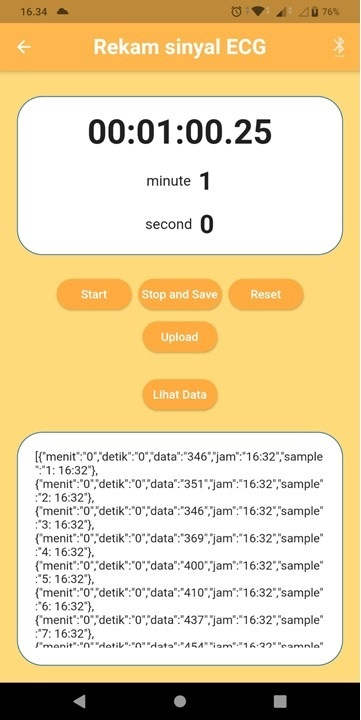
\includegraphics[width=1\linewidth]{img/percob/Slide14a}	  
		\caption{}		
	\end{subfigure}
	\begin{subfigure}{0.45\textwidth}
		\centering
		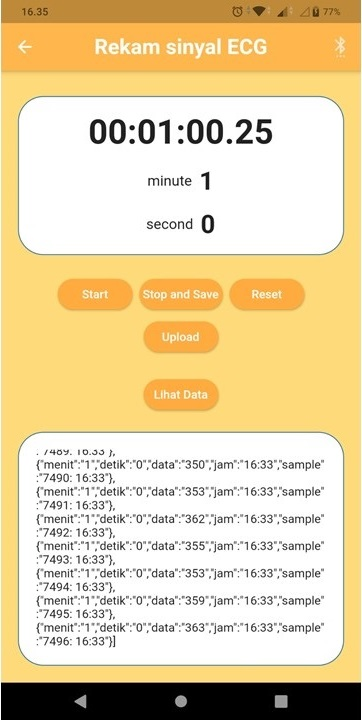
\includegraphics[width=1\linewidth]{img/percob/Slide14b.jpg}	  
		\caption{}		
	\end{subfigure}
	\caption{Percobaan 4: (a) Data awal yang diterima aplikasi, (b) Data akhir yang diterima aplikasi.}
	\label{fig:4.2.6}
\end{figure}
\vspace{1ex}
Pada percobaan keempat seperti yang diperlihatkan Gambar \ref{fig:4.2.6}, pada bagian kiri menunjukkan data awal yang diterima aplikasi yaitu 346 dan pada bagian kanan terdapat data terakhir yang diterima aplikasi yaitu 363. Jumlah data yang diterima aplikasi ditunjukkan pada nomor sampel data terakhir yaitu 7469. Kemudian berikut ini merupakan gambar percobaan terakhir.
\begin{figure}[H] \centering
	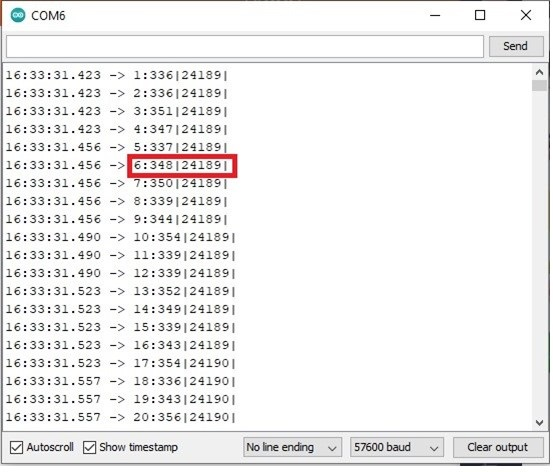
\includegraphics[width=0.7\textwidth]{img/percob/Slide9}
	
	(a)
	
	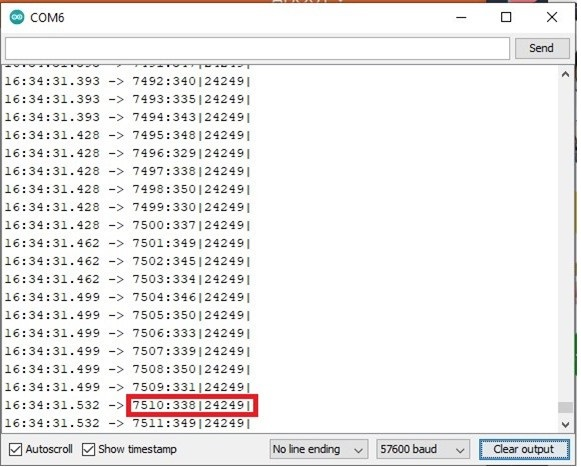
\includegraphics[width=0.7\textwidth]{img/percob/Slide10}
	
	(b)
	
	\caption{Percobaan 5 : (a)Data awal yang dikirim dari arduino, (b)Data akhir yang dikirim arduino.}
	\label{fig:4.2.7}
\end{figure}
\vspace{1ex}
Dapat diketahui dari gambar \ref{fig:4.2.7}, bagian (a) menunjukkan data awal yang terkirim yaitu 348 pada urutan sampel nomor 6, kemudian bagian (b) menunjukkan data terakhir yang terkirim yaitu 338 pada nomor sampel 7510. Apabila diperhitungkan melihat nomor sampel maka jumlah data yang terkirim adalah 7505 sampel.
\begin{figure}[H] \centering
	\begin{subfigure}{0.45\textwidth}
		\centering
		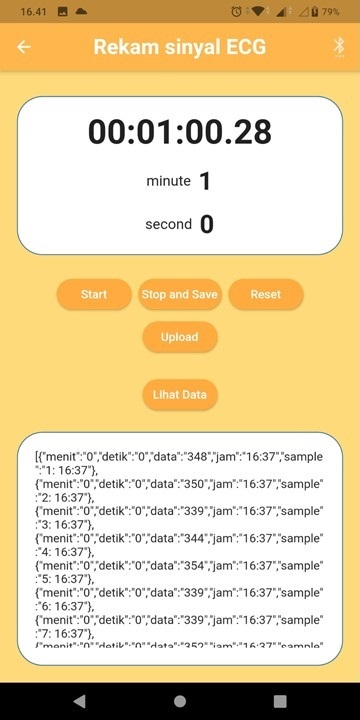
\includegraphics[width=1\linewidth]{img/percob/Slide15a}	  
		\caption{}		
	\end{subfigure}
	\begin{subfigure}{0.45\textwidth}
		\centering
		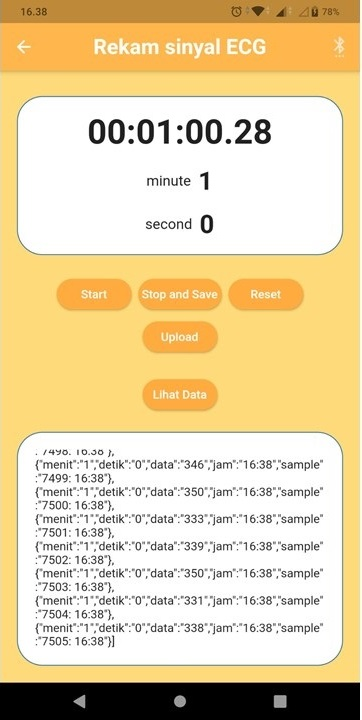
\includegraphics[width=1\linewidth]{img/percob/Slide15b.jpg}	  
		\caption{}		
	\end{subfigure}
	\caption{Percobaan 5: (a) Data awal yang diterima aplikasi, (b) Data akhir yang diterima aplikasi.}
	\label{fig:4.2.8}
\end{figure}
Pada percobaan terakhir didapatkan data seperti yang diperlihatkan Gambar \ref{fig:4.2.8}, pada bagian kiri menunjukkan data awal yang diterima aplikasi yaitu 348 dan pada bagian kanan terdapat data terakhir yang diterima aplikasi yaitu 338. Jumlah data yang diterima aplikasi ditunjukkan pada nomor sampel data terakhir yaitu 7505 sehingga jumlah data yang dikirim arduino sesuai dengan jumlah data yang diterima aplikasi. Untuk lebih jelasnya dapat dilihat pada tabel berikut.

\begin{table}[H]
	\begin{tabular}{|c|c|c|c|c|c|}
		\hline
		\multirow{3}{*}{\textbf{Uji ke-}} & \multicolumn{3}{|c|}{\textbf{Arduino}}& \multicolumn{1}{|c|}{\textbf{Aplikasi}}&
		\multicolumn{1}{|c|}{\textbf{Sesuai}}\\
		\cline{2-5} & \textbf{Nomor} & \textbf{Nomor} & \textbf{Jumlah}&\textbf{Jumlah} &  \\
		 & \textbf{sampel} & \textbf{sampel} & \textbf{sampel}& \textbf{sampel}&\\
		 &\textbf{awal}&\textbf{akhir}&&\textbf{diterima}&\\
		\hline1& 2 &7990 & 7989&7989&ya\\
		\hline2&6&7470&7465&7465 &ya  \\
		\hline3&6 &7530 &7525&7525&ya \\
		\hline4&1 &7496 &7496&7496&ya \\
		\hline3&6 &7510 &7505&7505&ya \\
		\hline
	\end{tabular}
\end{table}

\section{Pengujian Persentase Data Hilang}
\vspace{1ex}
Pada bagian ini, pengujian dilakukan dengan cara merekam data ECG yang dikirimkan oleh arduino. Pada pengujian ini menggunakan \textit{baudrate} sebesar 9600. Pengujian ini dilakukan untuk mengetahui seberapa banyak data yang hilang dengan cara membandingkan data yang dikirim oleh mikrokontroler arduino dengan data yang diterima oleh aplikasi. Berikut adalah tabel yang merupakan hasil percobaan selama 1 menit (Tabel \ref{tabel:4.1}).



\begin{table}[H]
	\caption{Tabel hasil percobaan persentase data hilang}
	\begin{tabular}{|c|c|c|c|c|c|}
		\hline
		\multicolumn{1}{|c|}{{\color[HTML]{000000} \textbf{Delay}}} & \multicolumn{1}{|c|}{\textbf{Uji}} &
		\multicolumn{1}{|c|}{ \textbf{Jumlah}} &
		\multicolumn{1}{|c|}{\textbf{Jumlah}} &
		\multicolumn{1}{|c|}{\textbf{\textit{Sampling}}}  & 
		\multicolumn{1}{|c|}{\textbf{Data}} \\
		(ms) &  \textbf{ke-}  & \textbf{rekaman}  & \textbf{data} & \textbf{\textit{rate}}  & \textit{hilang}\\
		&  &  &  \textbf{diterima} & & (\%) \\ \hline
		
		\multirow{5}{*}{5} &1& 15:00.09 &118317 &131 & 0.33 \\
		\cline{2-6}&2 &15.00.55 & 118214 &131 & 0.26\\ 
		\cline{2-6}&3 &15.00.73 & 118235 &131 & 0.33\\ 
		\cline{2-6}&4 &15.01.75 & 118229 &131 & 0.20\\ 
		\cline{2-6}&5 &15.00.34 & 118143 &131 & 0.18\\ 
		\hline
		\multirow{5}{*}{3} &1& 15:00.49 &161161 &179 & 0.24 \\
		\cline{2-6}&2 &15.14.86 & 162735 &180 & 0.32\\ 
		\cline{2-6}&3 &15.00.65 & 160370 &178 & 0.28\\ 
		\cline{2-6}&4 &15.00.54 & 161134 &179 & 0.31\\ 
		\cline{2-6}&5 &15.00.76 & 161743 &179 & 0.36\\ 
		\hline
		
	\end{tabular}
	\vspace{1ex}
	
	\label{tabel:4.1}
\end{table}
Tabel \ref{tabel:4.1} merupakan tabel yang memiliki 6 kolom yaitu Delay, Uji ke-, Jumlah Data dikirim, Jumlah Data diterima, Sampling
rate, Data hilang. Delay merupakan durasi jeda waktu pada loop
arduino. Jumlah Data dikirim merupakan banyak data yang dikirim
oleh arduino menuju aplikasi. Jumlah Data diterima merupakan banyak data yang telah sampai di aplikasi. \textit{Sampling rate} merupakan
banyak data yang diterima aplikasi pada setiap detik. Data hilang
merupakan jumlah data yang tidak berhasil sampai pada aplikasi.



Pada tabel \ref{tabel:4.1} terdapat kolom \textit{sampling rate} yang mana merupakan jumlah sample yang berhasil diterima oleh aplikasi dalam 1
detik. Perhitungan \textit{sampling rate} dengan cara perbandingan antara
jumlah data diterima dengan waktu uji. Selain itu juga terdapat
kolom data hilang dimana merupakan persentase jumlah data yang
tidak berhasil diterima oleh aplikasi. Perhitungan persentase data hilang adalah dengan cara membandingkan selisih jumlah data
dikirim dengan jumlah data diterima dengan jumlah data dikirim
kemudian dikalikan dengan 100 \%. Dari tabel 4.7 didapatkan persentasi data yang hilang adalah dibawah 1\%.

\vspace{1ex}


\section{Pengujian Kesesuian Grafik ECG}
\vspace{1ex}

Pada tahap ini, dilakukan pengujian dengan cara membandingkan grafik ECG yang telah ditampilkan oleh aplikasi android dengan grafik ECG yang ditampilkan oleh serial ploter yang merupakan tools dari Arduino IDE. Berikut adalah hasil grafik ECG yang ditampilkan oleh aplikasi Gambar \ref{fig:4.0}.

\begin{figure}[H] \centering
	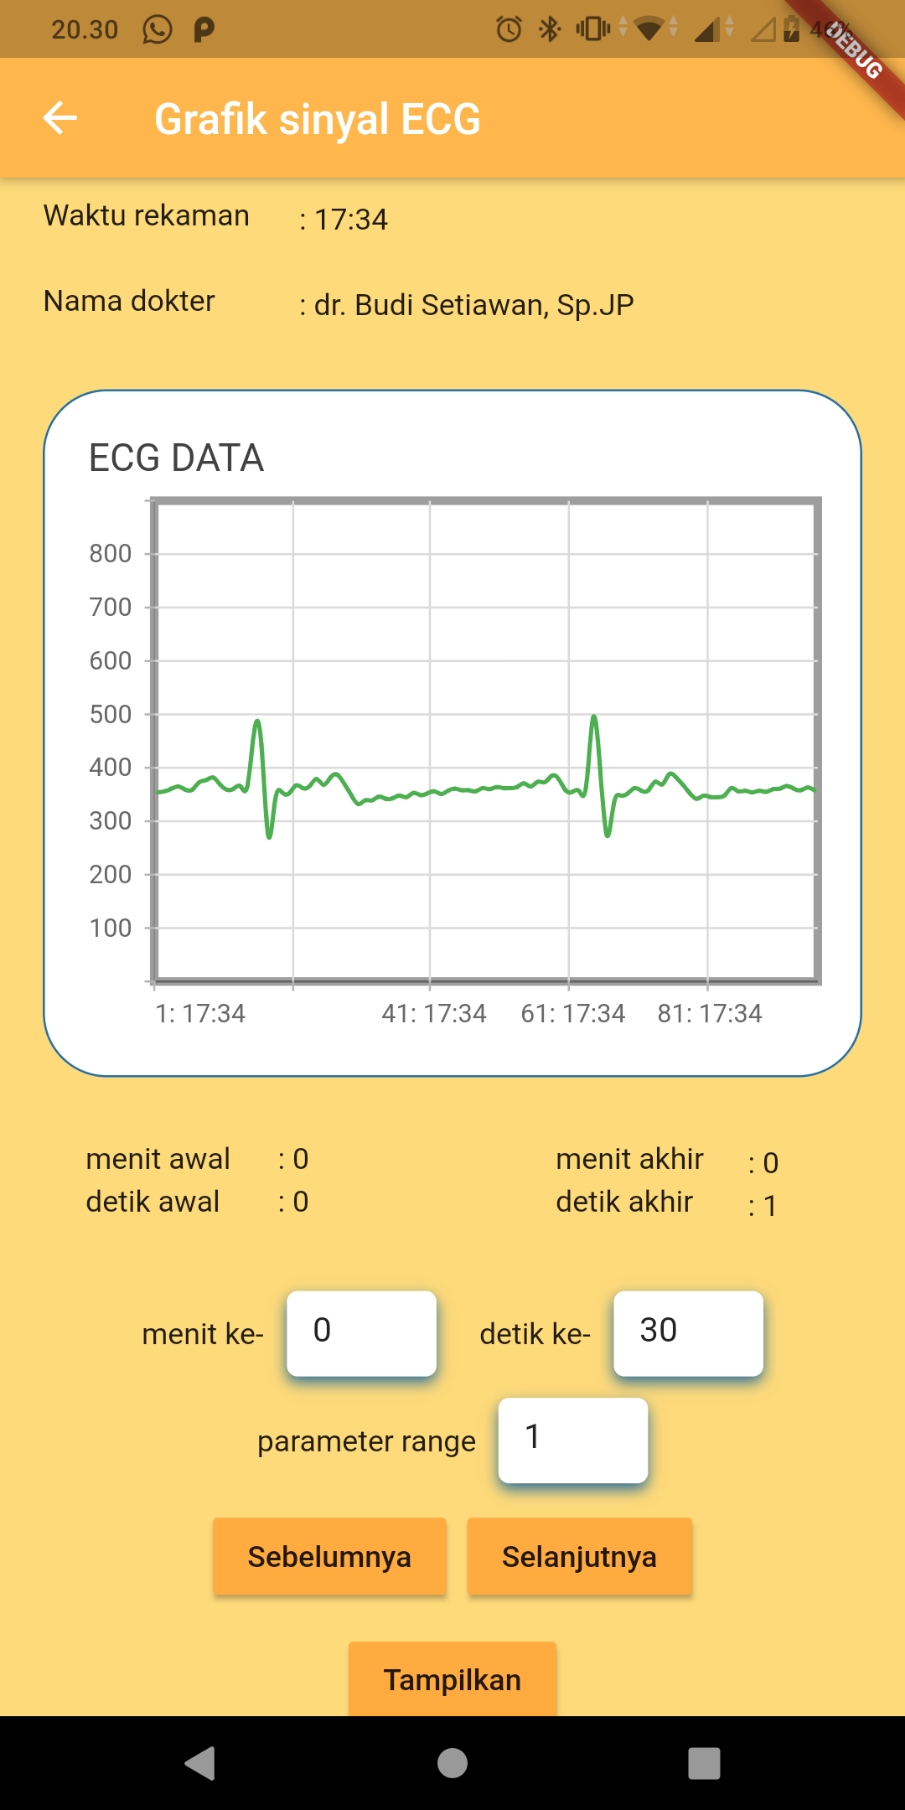
\includegraphics[width=0.45\textwidth]{img/grafikECGapps.jpg}
	\caption{Grafik ECG yang ditampilkan pada aplikasi.}
	\label{fig:4.0}
\end{figure}
Sedangkan grafik ECG yang ditampilkan pada serial ploter Arduino IDE ditunjukkan pada gambar berikut.
\begin{figure}[H] \centering
	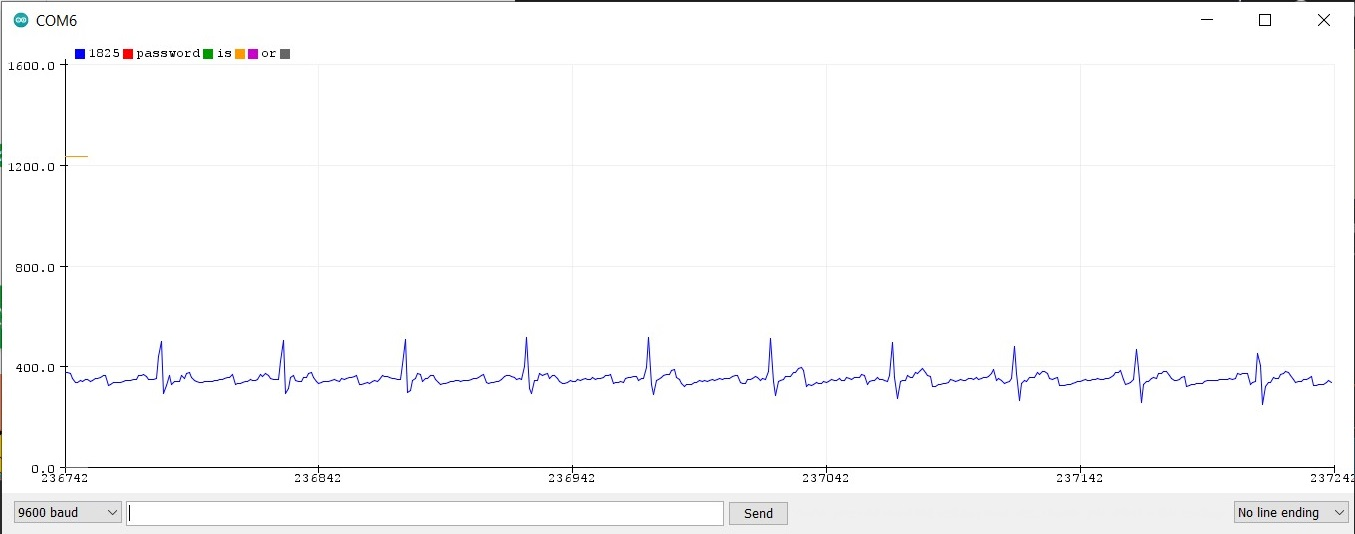
\includegraphics[width=1\textwidth]{img/ujisesuaidataIDE.jpg}
	\caption{Grafik ECG yang ditampilkan pada serial ploter Arduino IDE.}
	\label{fig:4.1}
\end{figure}

Berdasarkan kedua gambar diatas, apabila dibandingkan maka kedua gambar tersebut cukup mirip. Dengan demikian berarti hasil grafik ECG yang ditampilkan oleh aplikasi android cukup sesuai dengan grafik ECG yang ditampilkan oleh serial ploter Arduino IDE.
\vspace{1ex}


\cleardoublepage
\chapter{PENUTUP}
\vspace{1ex}

\section{Kesimpulan}
\vspace{1ex}
Pada penelitian ini, dilakukan pengambilan data ECG dengan menggunakan sensor AD8232 dan kemudian dikirimkan menuju aplikasi android melalui modul bluetooth HC-05. Pengambilan data tersebut dilakukan selama 15 menit. Setelah semua data diterima oleh aplikasi, data kemudian akan diupload menuju database. Data yang telah diupload di database dapat diakses oleh Dokter Spesialis agar dapat diberi diagnosa melalui aplikasi android. Aplikasi android juga memiliki fitur chat sehingga pasien dapat berkonsultasi dengan dokter.

Dari hasil pengujian yang sudah dilakukan pada bab sebelumnya, dapat ditarik beberapa kesimpulan sebagai berikut:
\begin{enumerate}[nolistsep]
	
	\item Aplikasi sudah dapat merekam data ECG dari arduino melalui modul bluetooth HC-05, menampilkan garfik ECG, chatting.
	
	\item Hasil pengujian untuk menghitung data yang hilang menunjukkan bahwa data yang hilang setiap sampling adalah kurang dari 1\%.
	
	\item Dari hasil pengujian kesesuaian grafik ECG menunjukkan bahwa hasil grafik ECG yang ditampilkan oleh aplikasi sudah cukup sesuai.
	
	\item Aplikasi dapat merekam data selama 15 menit dengan frekuensi sampling 50 sampel per detik yaitu menggunakan baudrate 9600 pada HC-05 dan delay 10 ms pada arduino
	
	\item Semakin besar frekuensi sampling maka semakin besar kemungkinan force close pada aplikasi
	
	\item Durasi upload data menuju database tergantung pada kondisi jaringan internet
	

	

\end{enumerate}
\vspace{1ex}

\section{Saran}
\vspace{1ex}

Untuk pengembangan penelitian selanjutnya terdapat beberapa saran sebagai berikut :
\vspace{1ex}
\begin{enumerate}[nolistsep]
	\item Mengirim data ECG menuju aplikasi selain menggunakan bluetooth,
	\item Menambah fitur aplikasi untuk dapat mendeteksi adanya aritmia dari data ECG hasil rekaman.
\end{enumerate}


\cleardoublepage

% Daftar pustaka
\renewcommand*\bibname{DAFTAR PUSTAKA}
\addcontentsline{toc}{chapter}{\bibname}
\titlespacing*{\chapter}{0pt}{-4ex}{2ex}
\appendix
\bibliographystyle{ieeetr}
\bibliography{TA}
\cleardoublepage


% Biografi penulis
\begin{center}
\Large\textbf{BIOGRAFI PENULIS}
\end{center}
\vspace{1ex}

\begin{wrapfigure}{L}{0.3\textwidth}
	\centering
	\vspace{-3ex}	
	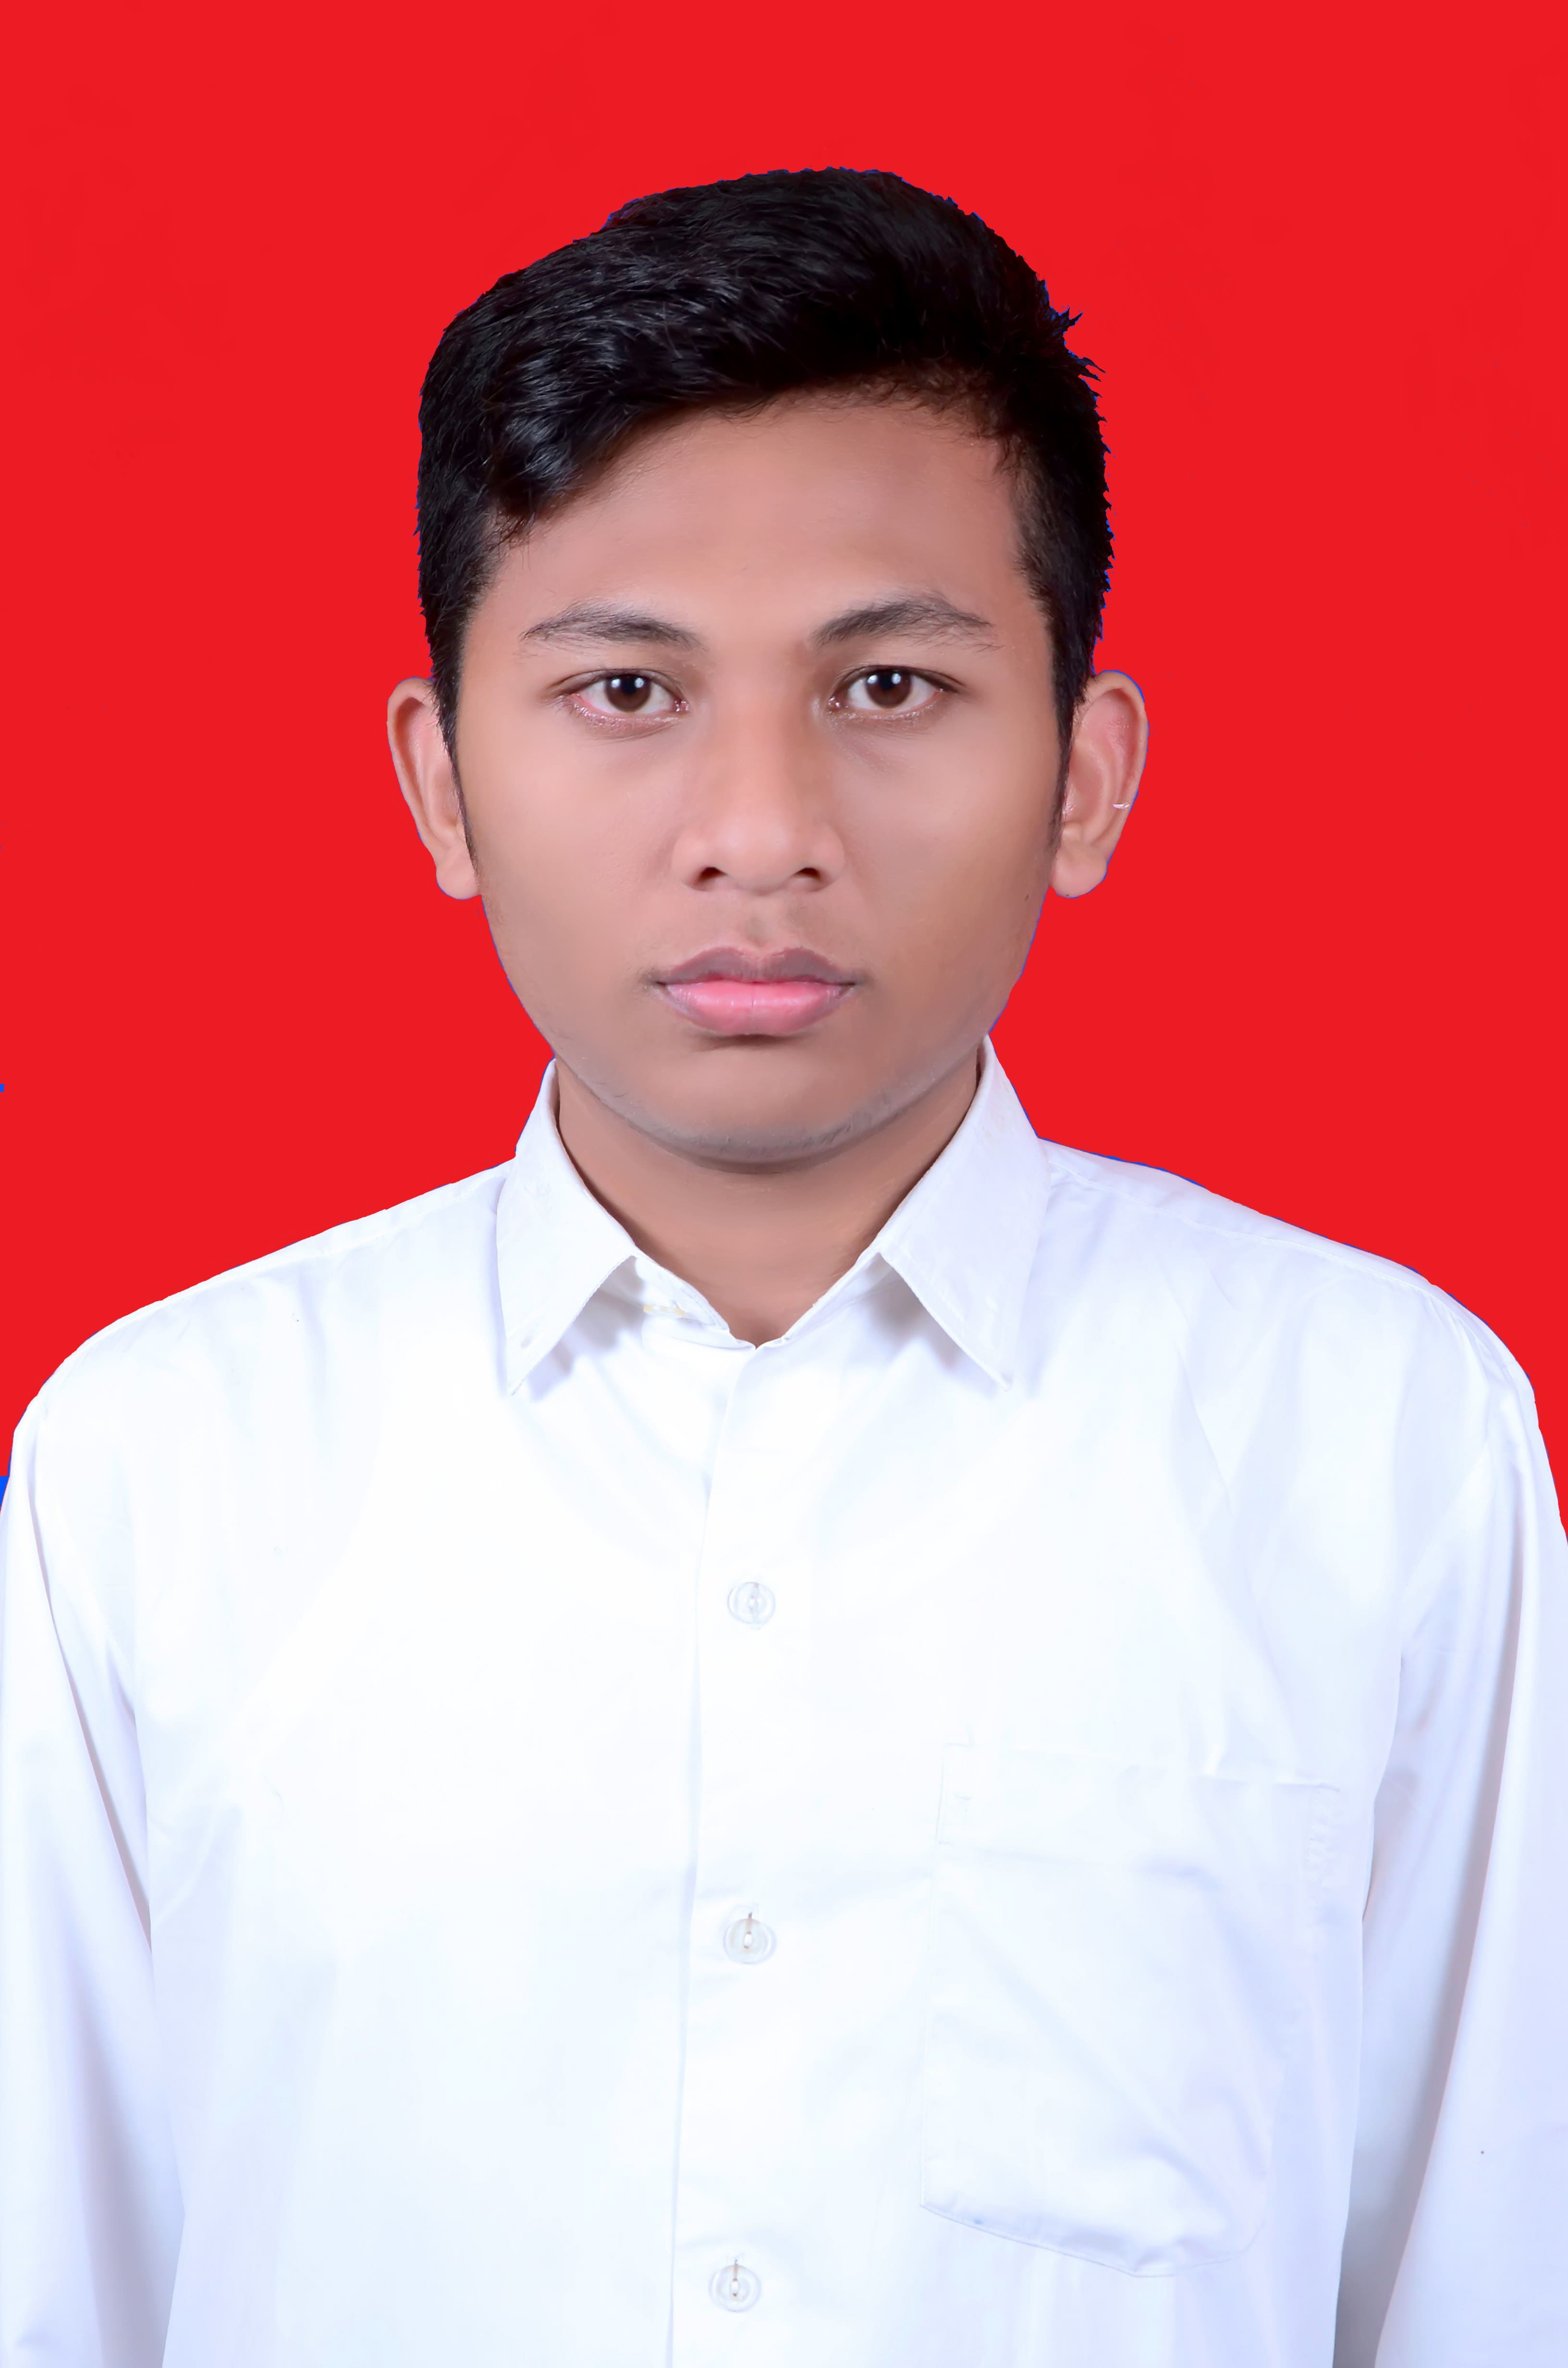
\includegraphics[width=0.31\textwidth]{img/robby.jpg}
	\vspace{-4ex}
\end{wrapfigure}
\noindent Robby Aldriyanto Raffly, atau biasa dipanggil Robby, lahir di Nganjuk Jawa Timur pada tanggal 12 Juli 1998. Merupakan anak tunggal. Penulis lulus dari SMP Negeri 2 Nganjuk dan melanjutkan ke SMA Negeri 2 Nganjuk. Penulis melanjutkan ke jenjang strata satu di Departemen Teknik Komputer Fakultas Teknologi Elektro dan Informatika Cerdas ITS. Dalam masa kuliah, penulis tertarik dengan pengembangan \textit{Mobile Apps} dan \textit{Machine Learning}. Penulis pernah aktif menjadi Staf Departemen Muamalah KALAM ELITS serta menjadi Koordinator Keamanan dan Perizinan MAGE 4. Bagi pembaca yang memiliki kritik, saran, atau pertanyaan mengenai tugas akhir ini dapat menghubungi penulis melalui email robbyaraffly12@gmail.com.
\addcontentsline{toc}{chapter}{Biografi Penulis}
\cleardoublepage

\end{document}